\section{Модальное управление}
\subsection{Модальный регулятор}
Рассмотрим модальный регулятор вида $u = Kx$. Согласно (\ref{eq:controlability_matrix}), система является 
полностью управляемой. Таким образом, любой спектр замкнутой системы является достижимым. 
Выберем желаемый спектр для замкнутой регулятор системы $\sigma_1 = \begin{bmatrix}-2 & -2 & -3 & -3\end{bmatrix}$. 
Для реализации регулятора, обеспечивающего заданный спектр, воспользуемся уравнением Сильвестра: 
\begin{equation}
    \begin{cases}
        AP - P\Gamma = BY \\
        K = -YP^{-1} 
    \end{cases}
\end{equation}
где $\Gamma$ -- матрица с желаемым спектром. 

Решим данное уравнение с помощью пакета \texttt{cvx} в MATLAB, в результате получаем матрицу регулятора $K$:
\begin{equation}
    K = \begin{bmatrix}
    484.11  & 806.85  & -7714.17  & -1732.95 \\ 
    \end{bmatrix}
\end{equation} 
Проверим правильность полученного результата, вычислив собственные числа замкнутой системы $A + BK$: 
\begin{equation}
    \sigma(A + BK) = \begin{bmatrix}
    -2.00 \\ 
    -2.00 \\ 
    -3.00 \\ 
    -3.00 \\ 
    \end{bmatrix}
\end{equation}
Получены желаемые собственные числа, что подтверждает правильность полученного результата. 
Рассмотрим работу регулятора на линейной модели системы при отсутствии внешних возмущений и 
небольшом начальном отклонении от равновесного состояния ($\theta_0 = 0.2$). Схема моделирования приведена на 
рисунке \ref{fig:modal_control_scheme_linear}. Результаты моделирования приведены на 
рисунке \ref{fig:modal_control_linear_out}.

\begin{figure}[ht!]
    \centering
    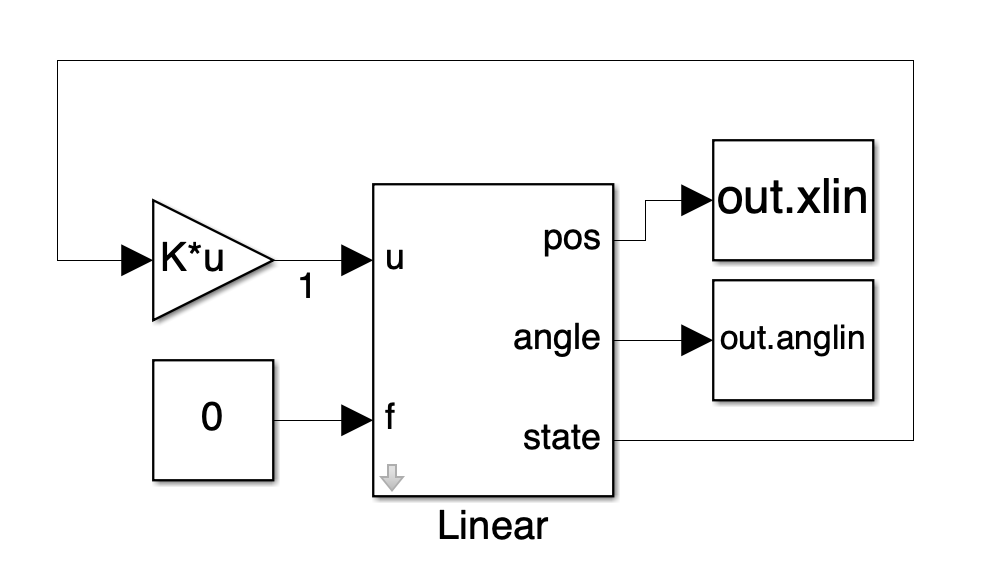
\includegraphics[width=0.7\textwidth]{media/modal_control_linear_scheme.png}
    \caption{Схема моделирования линейной модели системы с модальным регулятором}
    \label{fig:modal_control_scheme_linear}
\end{figure}
\begin{figure}[ht!]
    \centering
    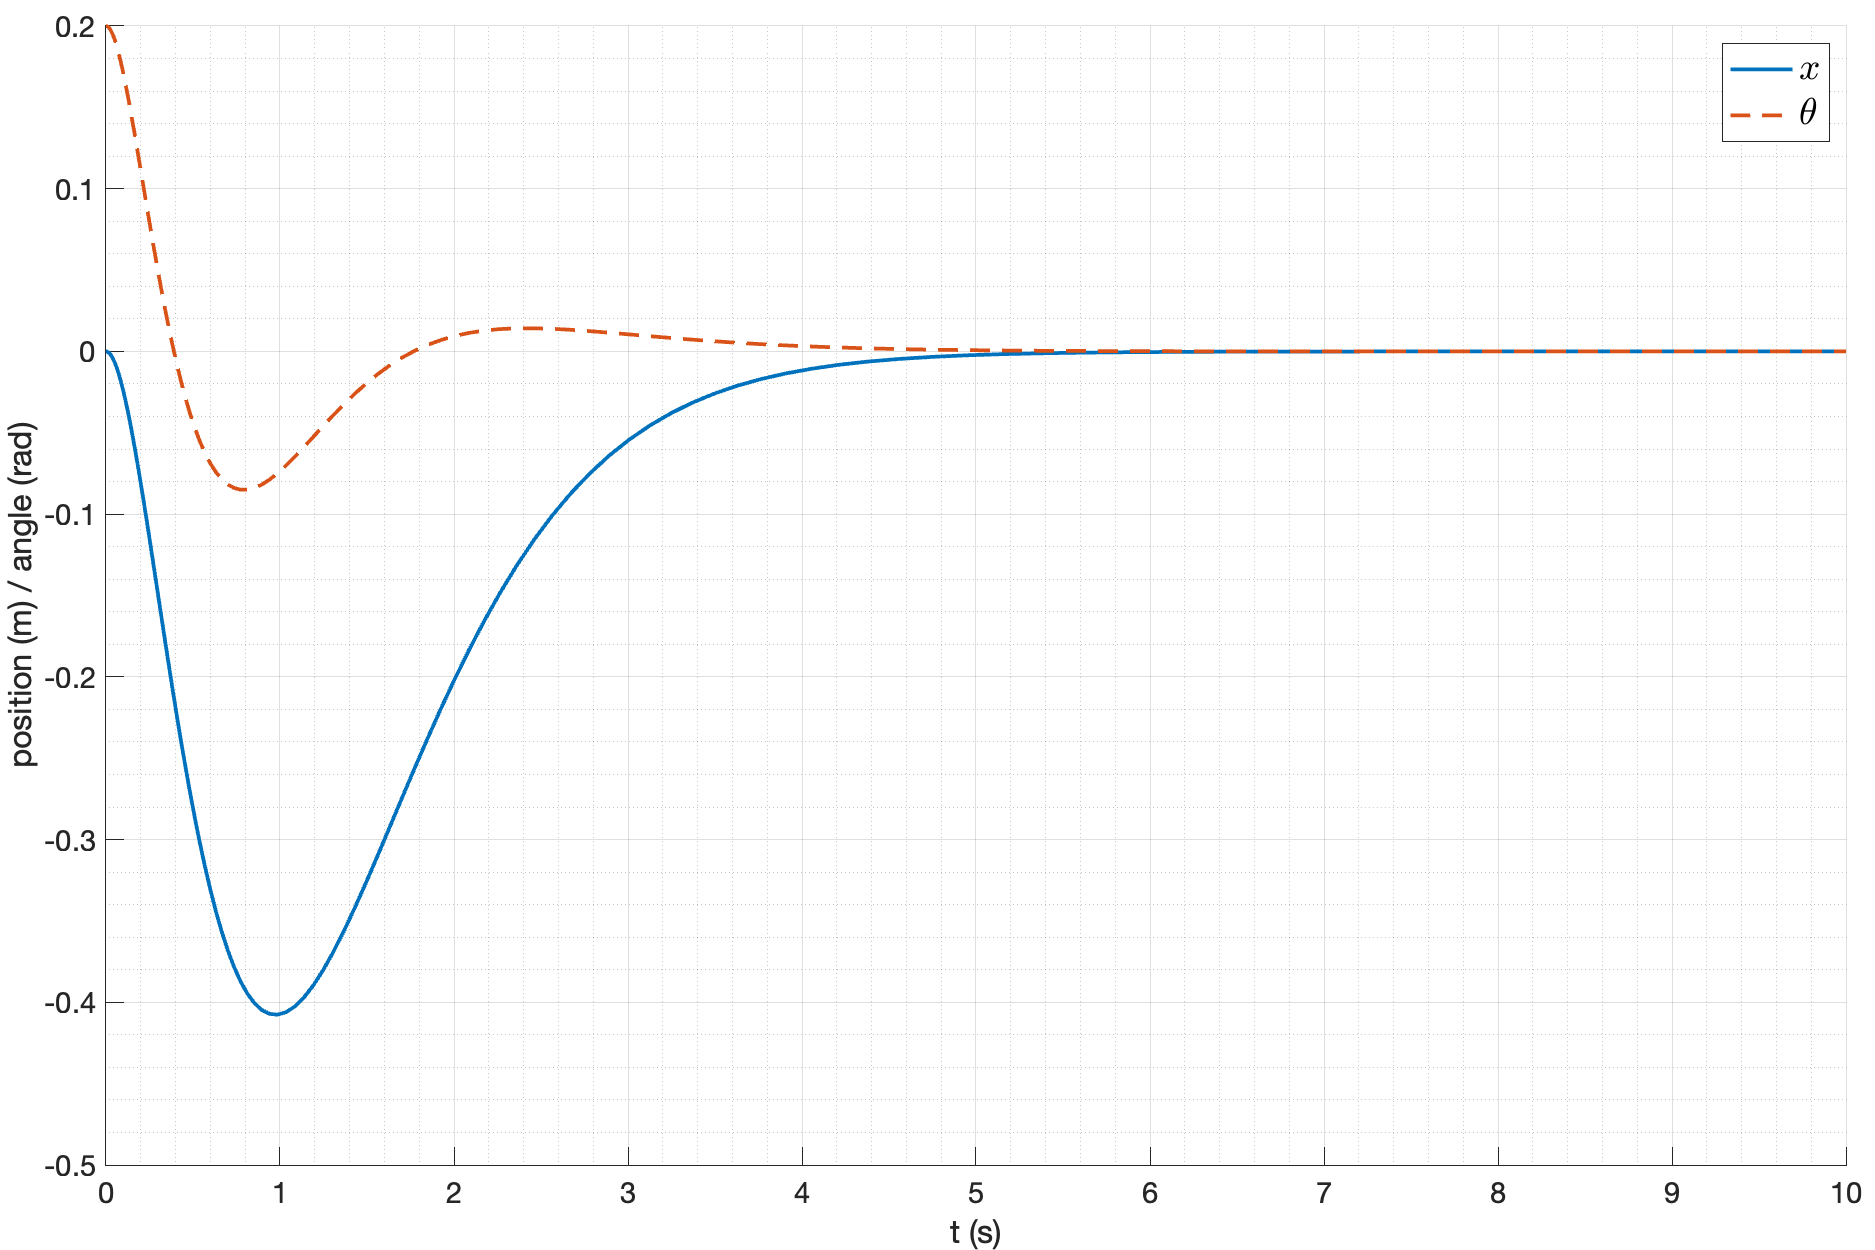
\includegraphics[width=0.8\textwidth]{media/plots/modal_control/linear_out_0.png}
    \caption{Результаты моделирования линейной модели системы с модальным регулятором}
    \label{fig:modal_control_linear_out}
\end{figure}

Можно заметить, что система приходит в равновесное состояние. Теперь попробуем использовать этот же 
модальный регулятор на нелинейной модели системы. Схема моделирования приведена на
рисунке \ref{fig:modal_control_scheme_nonlinear}. Результаты моделирования приведены на
рисунке \ref{fig:modal_control_nonlinear_out}.


\begin{figure}[ht!]
    \centering
    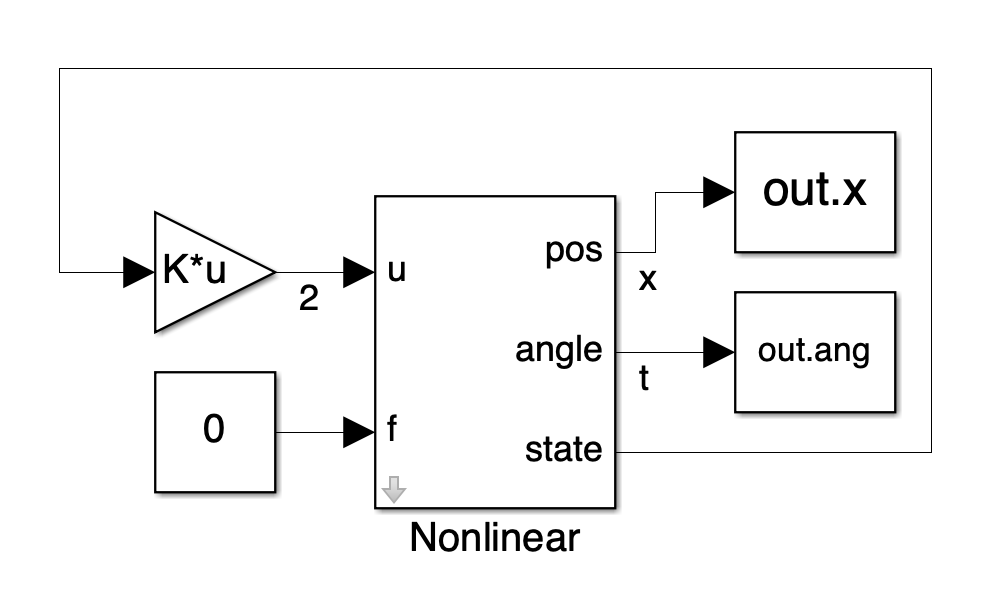
\includegraphics[width=0.7\textwidth]{media/modal_control_scheme.png}
    \caption{Схема моделирования нелинейной модели системы с модальным регулятором}
    \label{fig:modal_control_scheme_nonlinear}
\end{figure}
\begin{figure}[ht!]
    \centering
    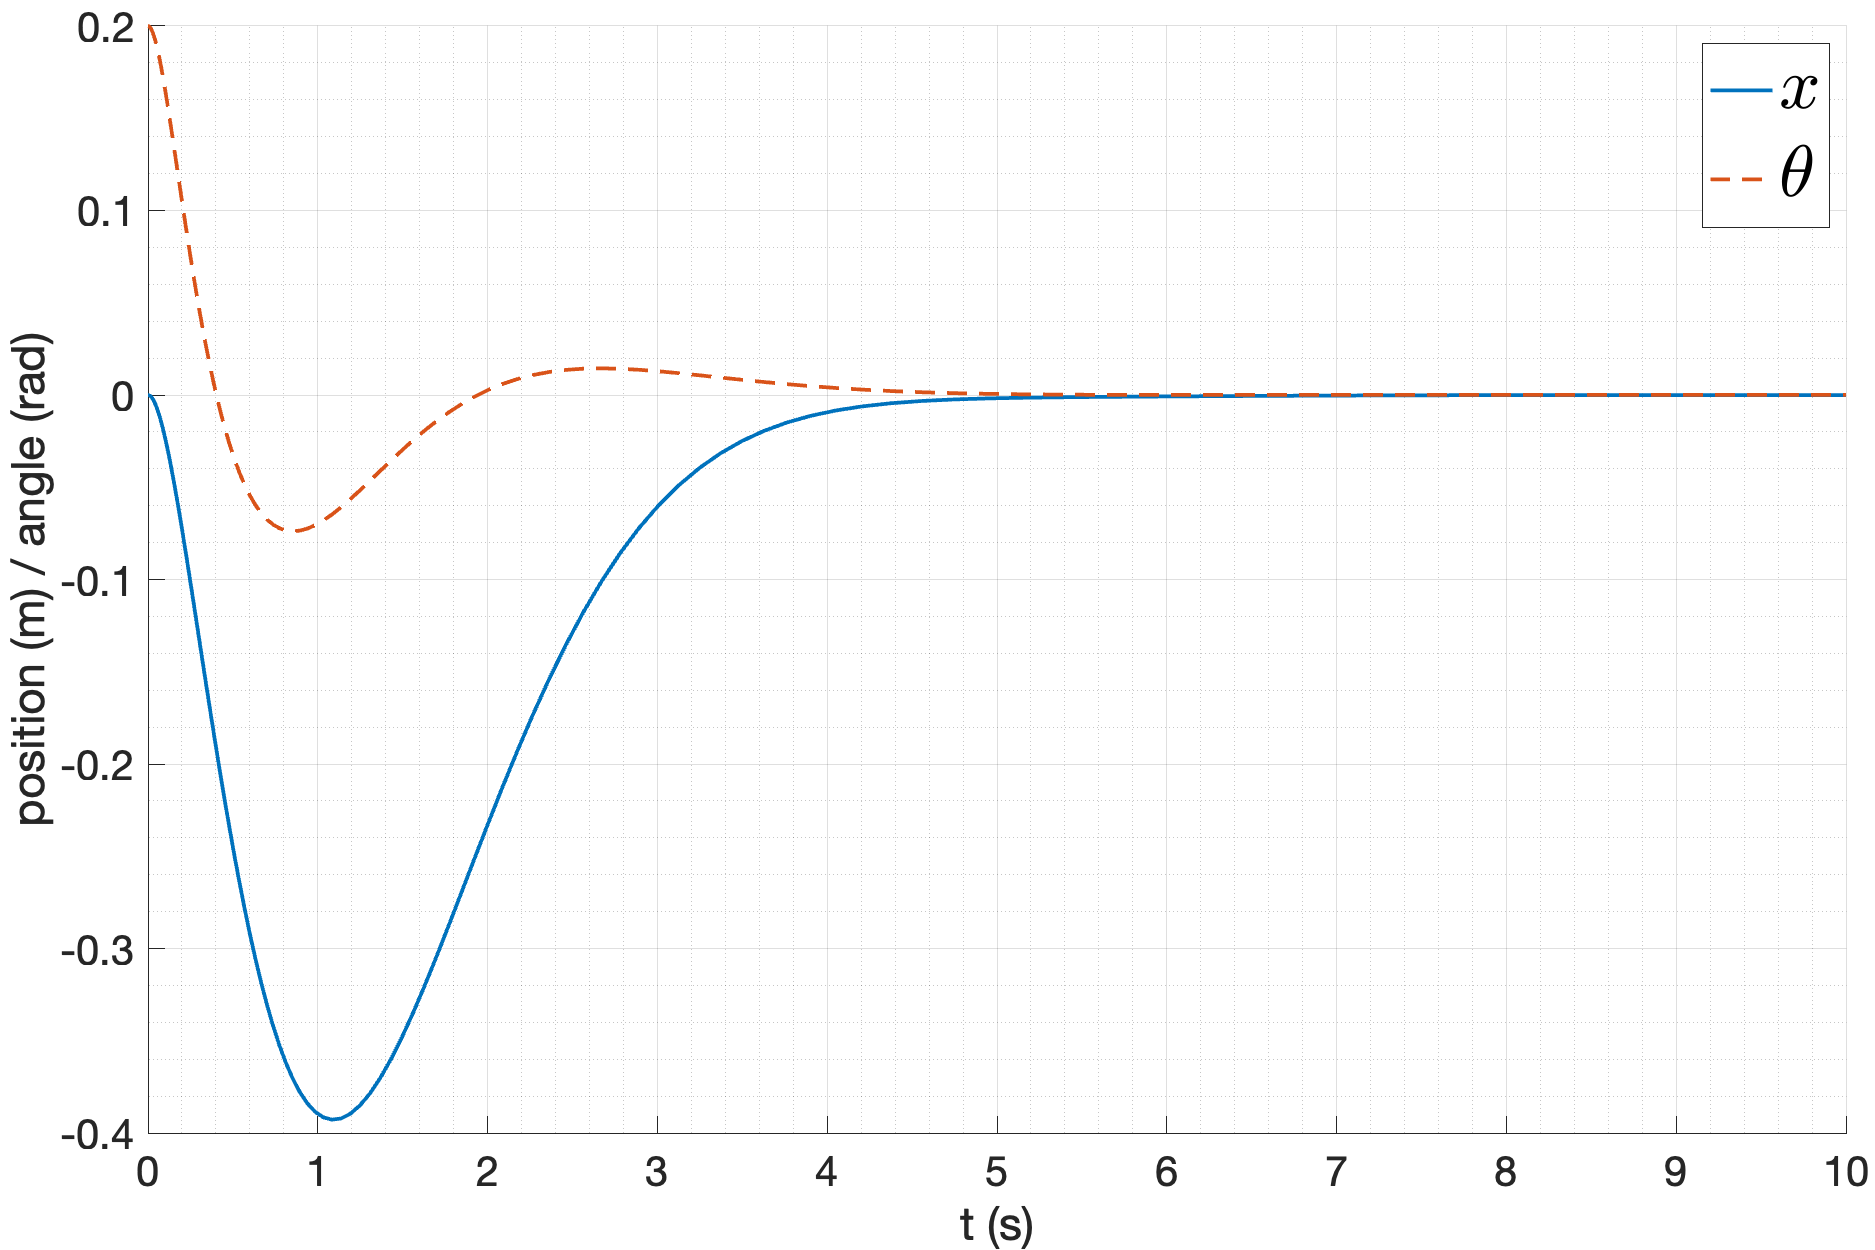
\includegraphics[width=0.8\textwidth]{media/plots/modal_control/out_0.png}
    \caption{Результаты моделирования нелинейной модели системы с модальным регулятором}
    \label{fig:modal_control_nonlinear_out}
\end{figure}

Рассмотрим различия между движением линейной и нелинейной модели системы. График различий в движении
представлен на рисунке \ref{fig:modal_control_cmp}.
\begin{figure}[ht!]
    \centering
    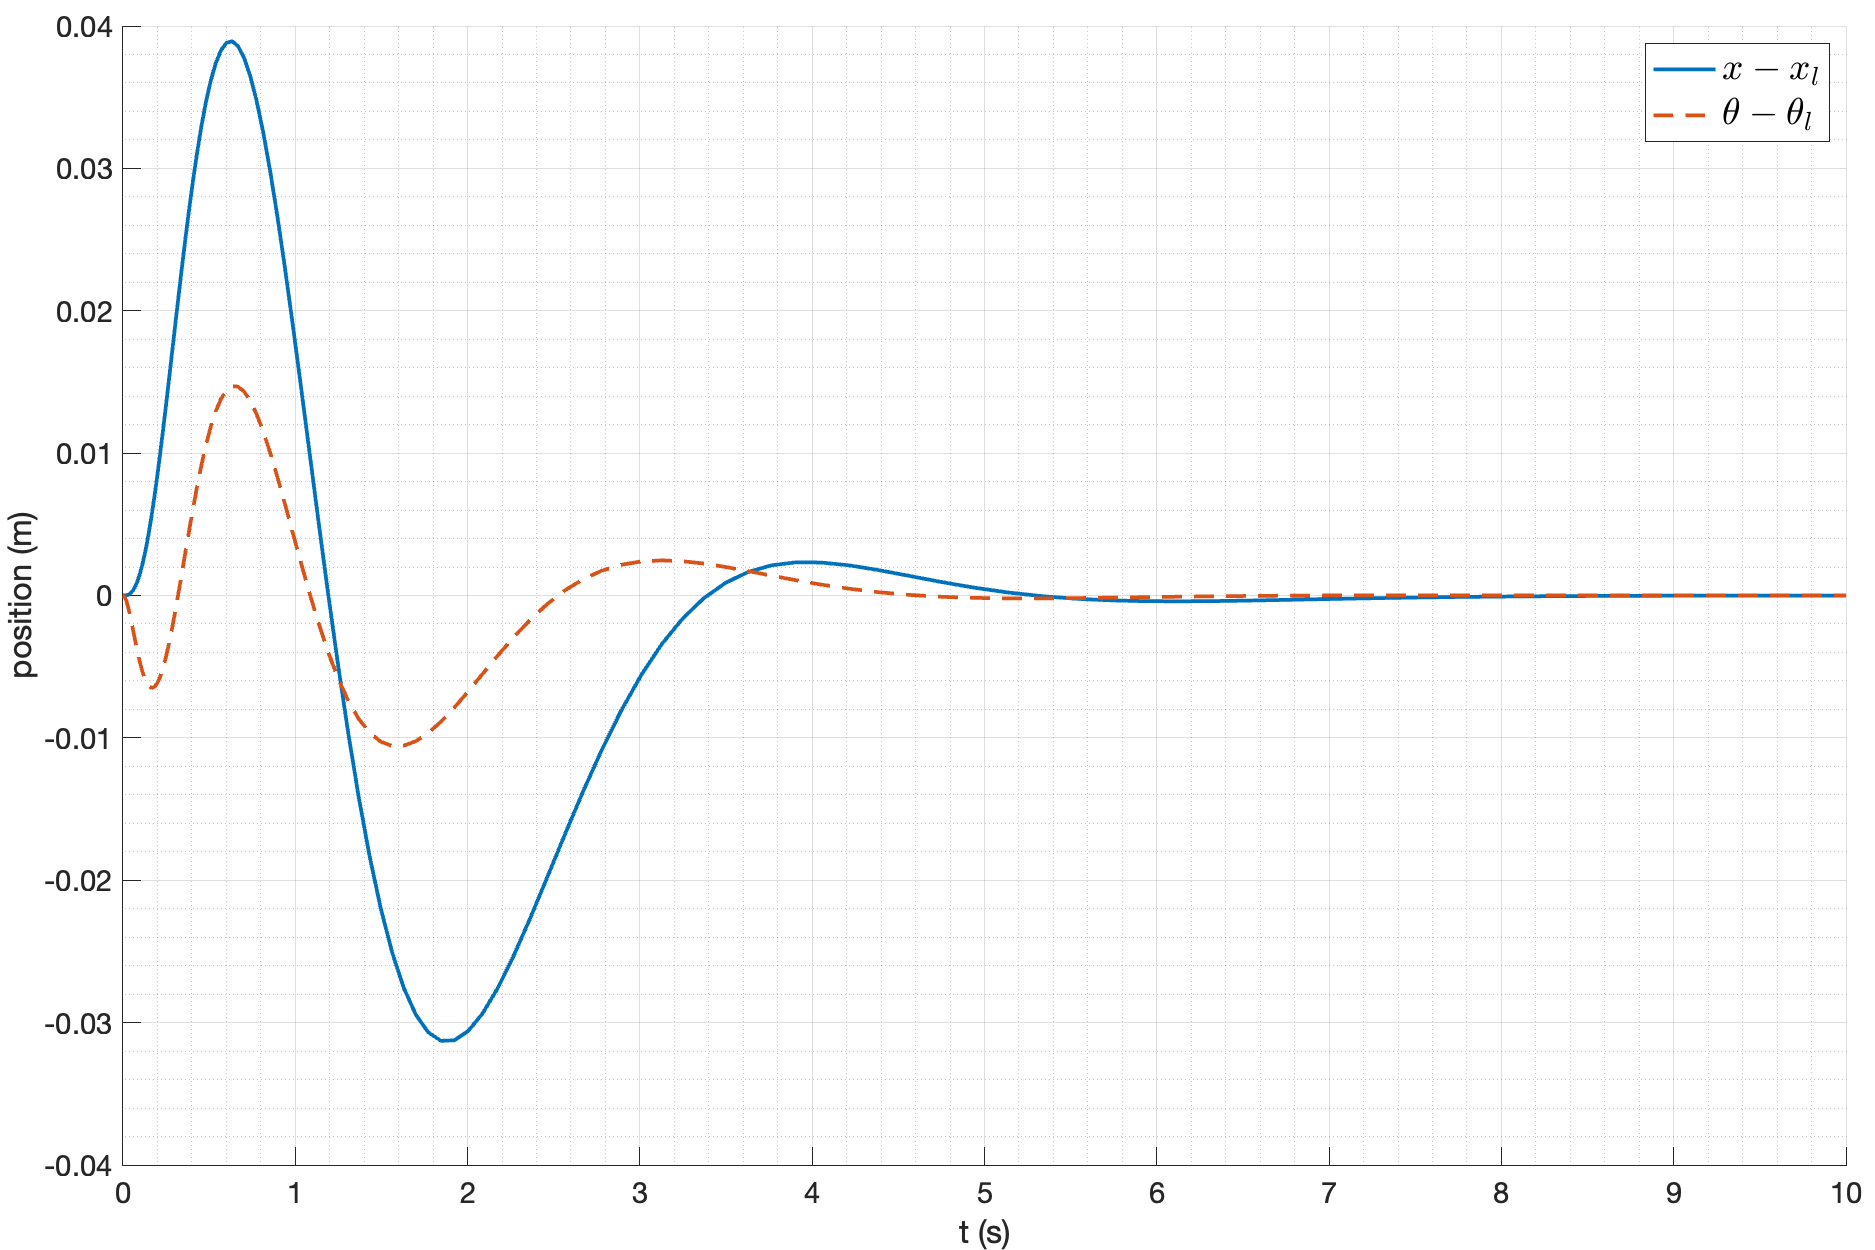
\includegraphics[width=0.8\textwidth]{media/plots/modal_control/cmp_0.png}
    \caption{Различия в движении линейной и нелинейной модели системы с модальным регулятором}
    \label{fig:modal_control_cmp}
\end{figure}
Видно, что различие между углом отклонения маятника не превышает $2 \cdot 10^{-2}$ радиан, а различие между
координатами тележки не превышает $4\cdot10^{-2}$ метра. Данный результат можно считать удовлетворительным, 
регулятор, синтезированный для линейной модели системы, обеспечивает приемлемое качество управления 
нелинейной модели системы. 

\FloatBarrier
\subsection{Исследование устойчивости при различных начальных условиях}
Проверим работу данного регулятора при различных начальных условиях. 
В качестве начальных условий возьмем различные начальные углы отклонения маятника $\theta_0 \in \begin{bmatrix}0.3, 0.7, 0.9, 1.0, 1.1, 1.2\end{bmatrix}$. Результаты 
моделирования приведены на рисунке \ref{fig:modal_control_initials}. 
\begin{figure}[ht!]
    \centering
    \begin{subfigure}[b]{0.45\textwidth}
        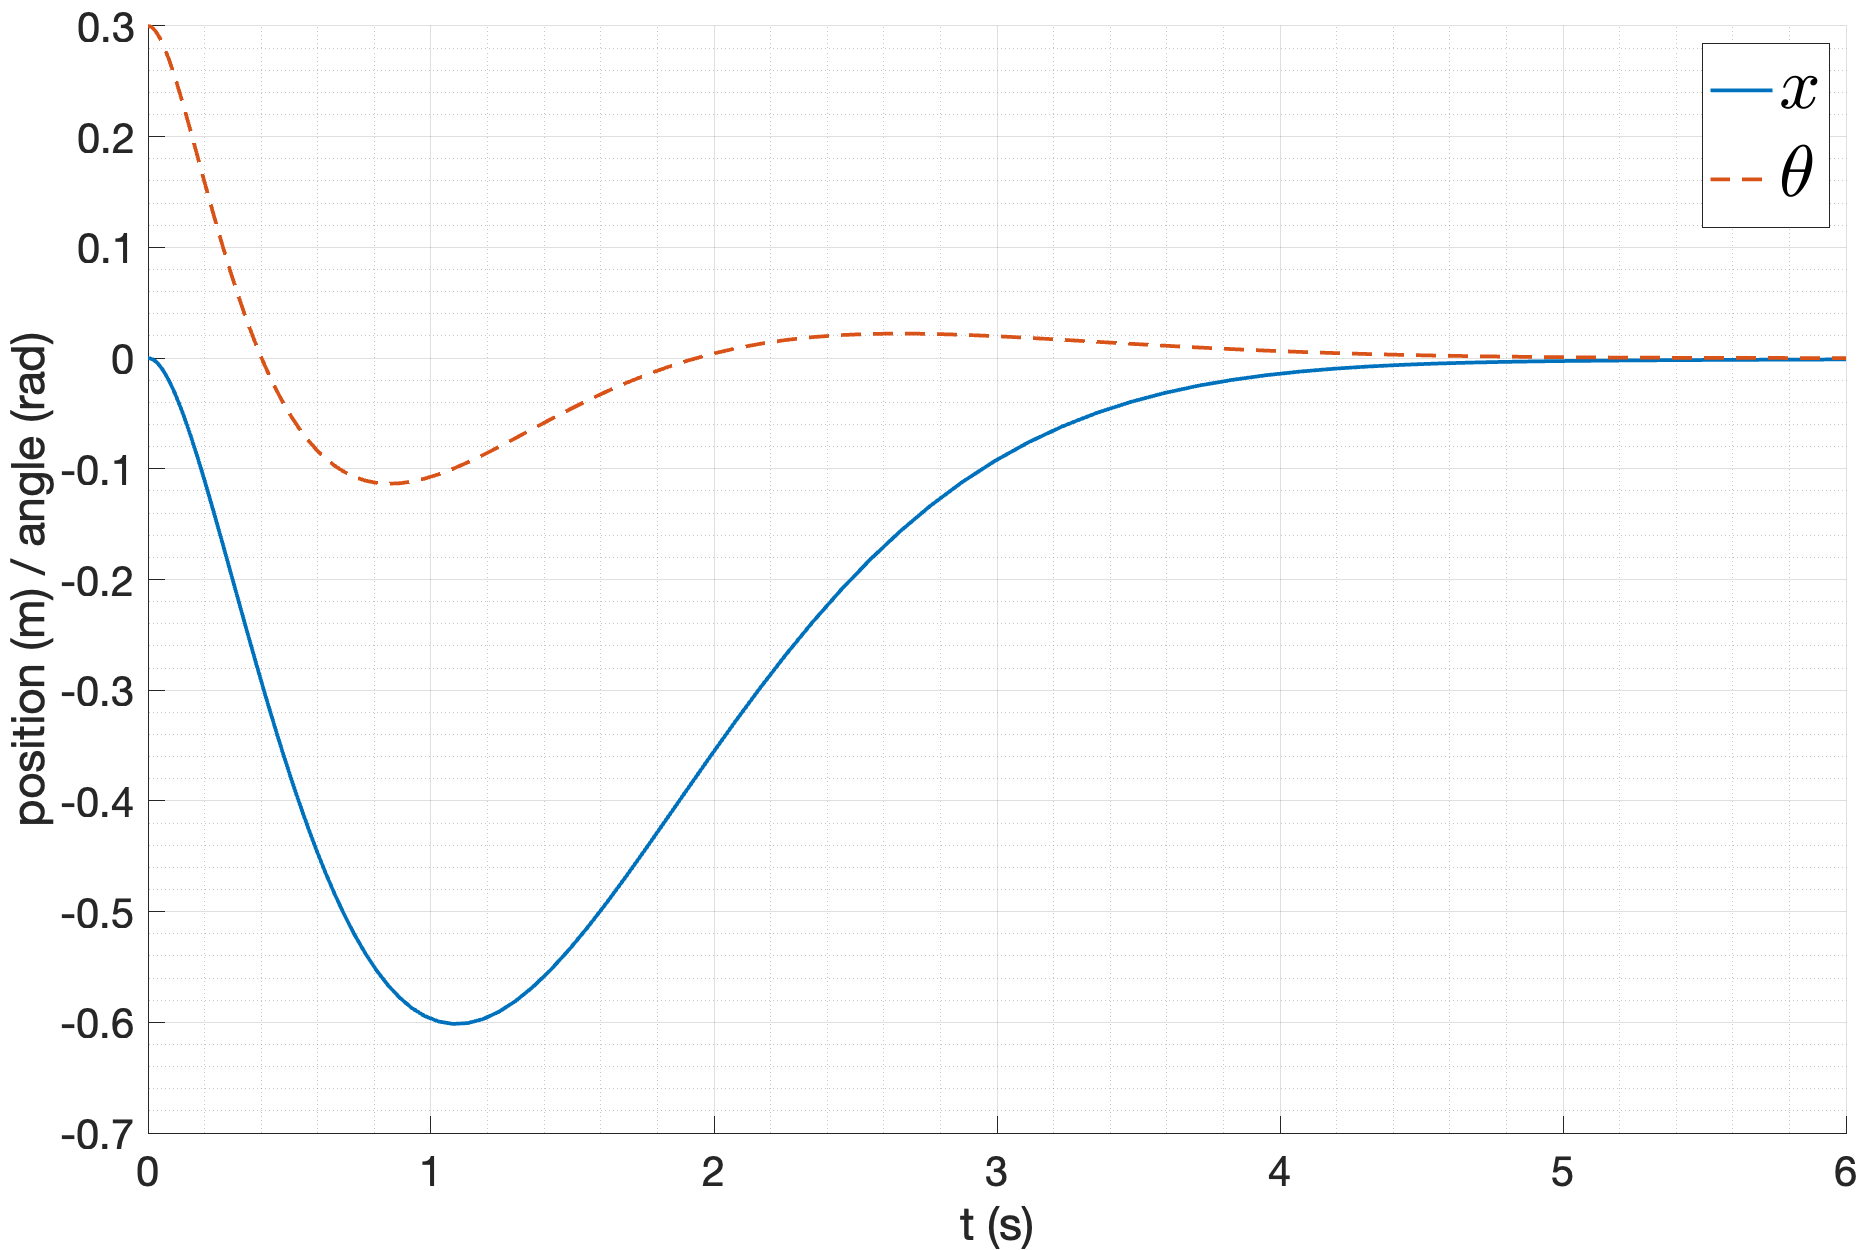
\includegraphics[width=\textwidth]{media/plots/modal_control/out_1.png}
        \caption{$\theta_0 = 0.3$}
    \end{subfigure}
    \begin{subfigure}[b]{0.45\textwidth}
        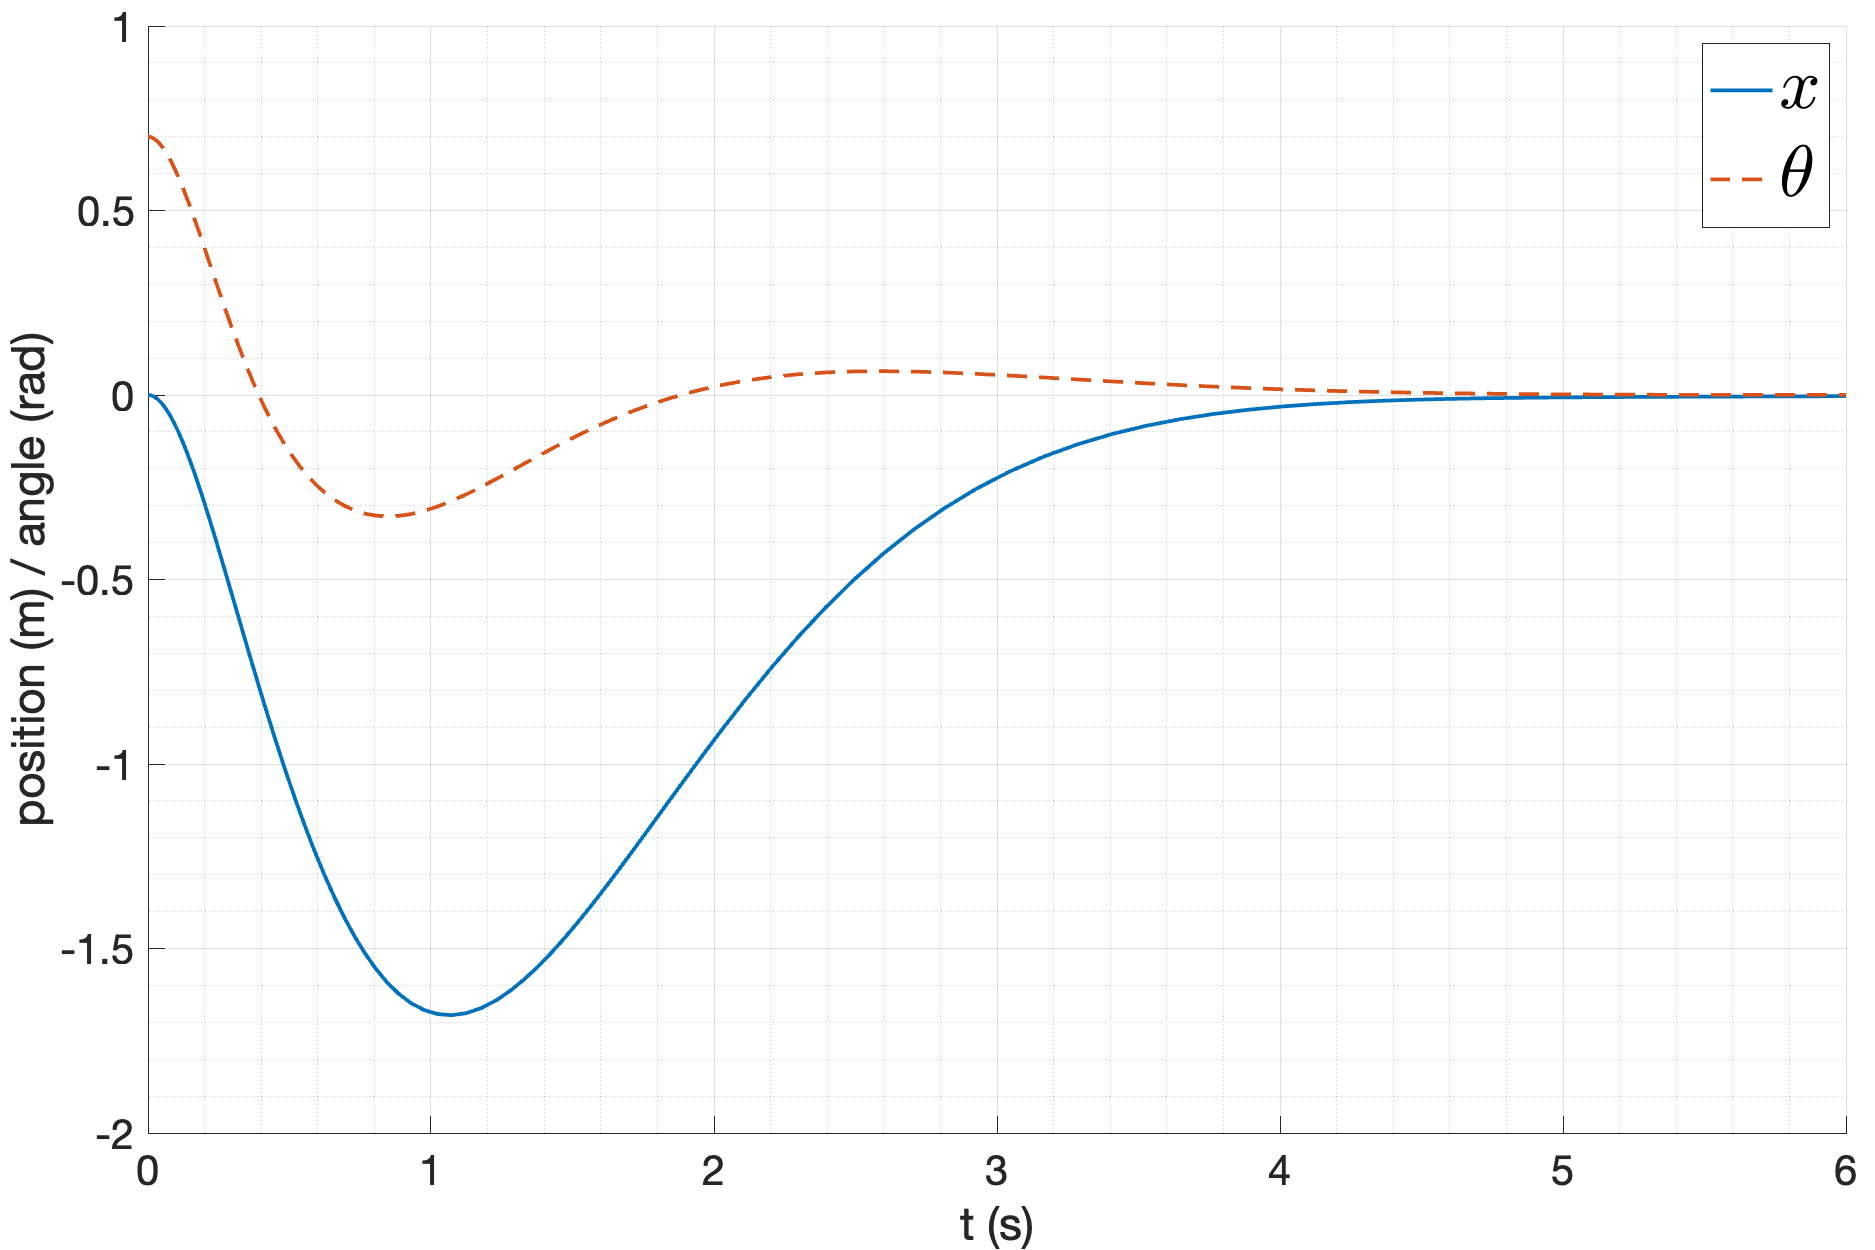
\includegraphics[width=\textwidth]{media/plots/modal_control/out_2.png}
        \caption{$\theta_0 = 0.7$}
    \end{subfigure}
    \begin{subfigure}[b]{0.45\textwidth}
        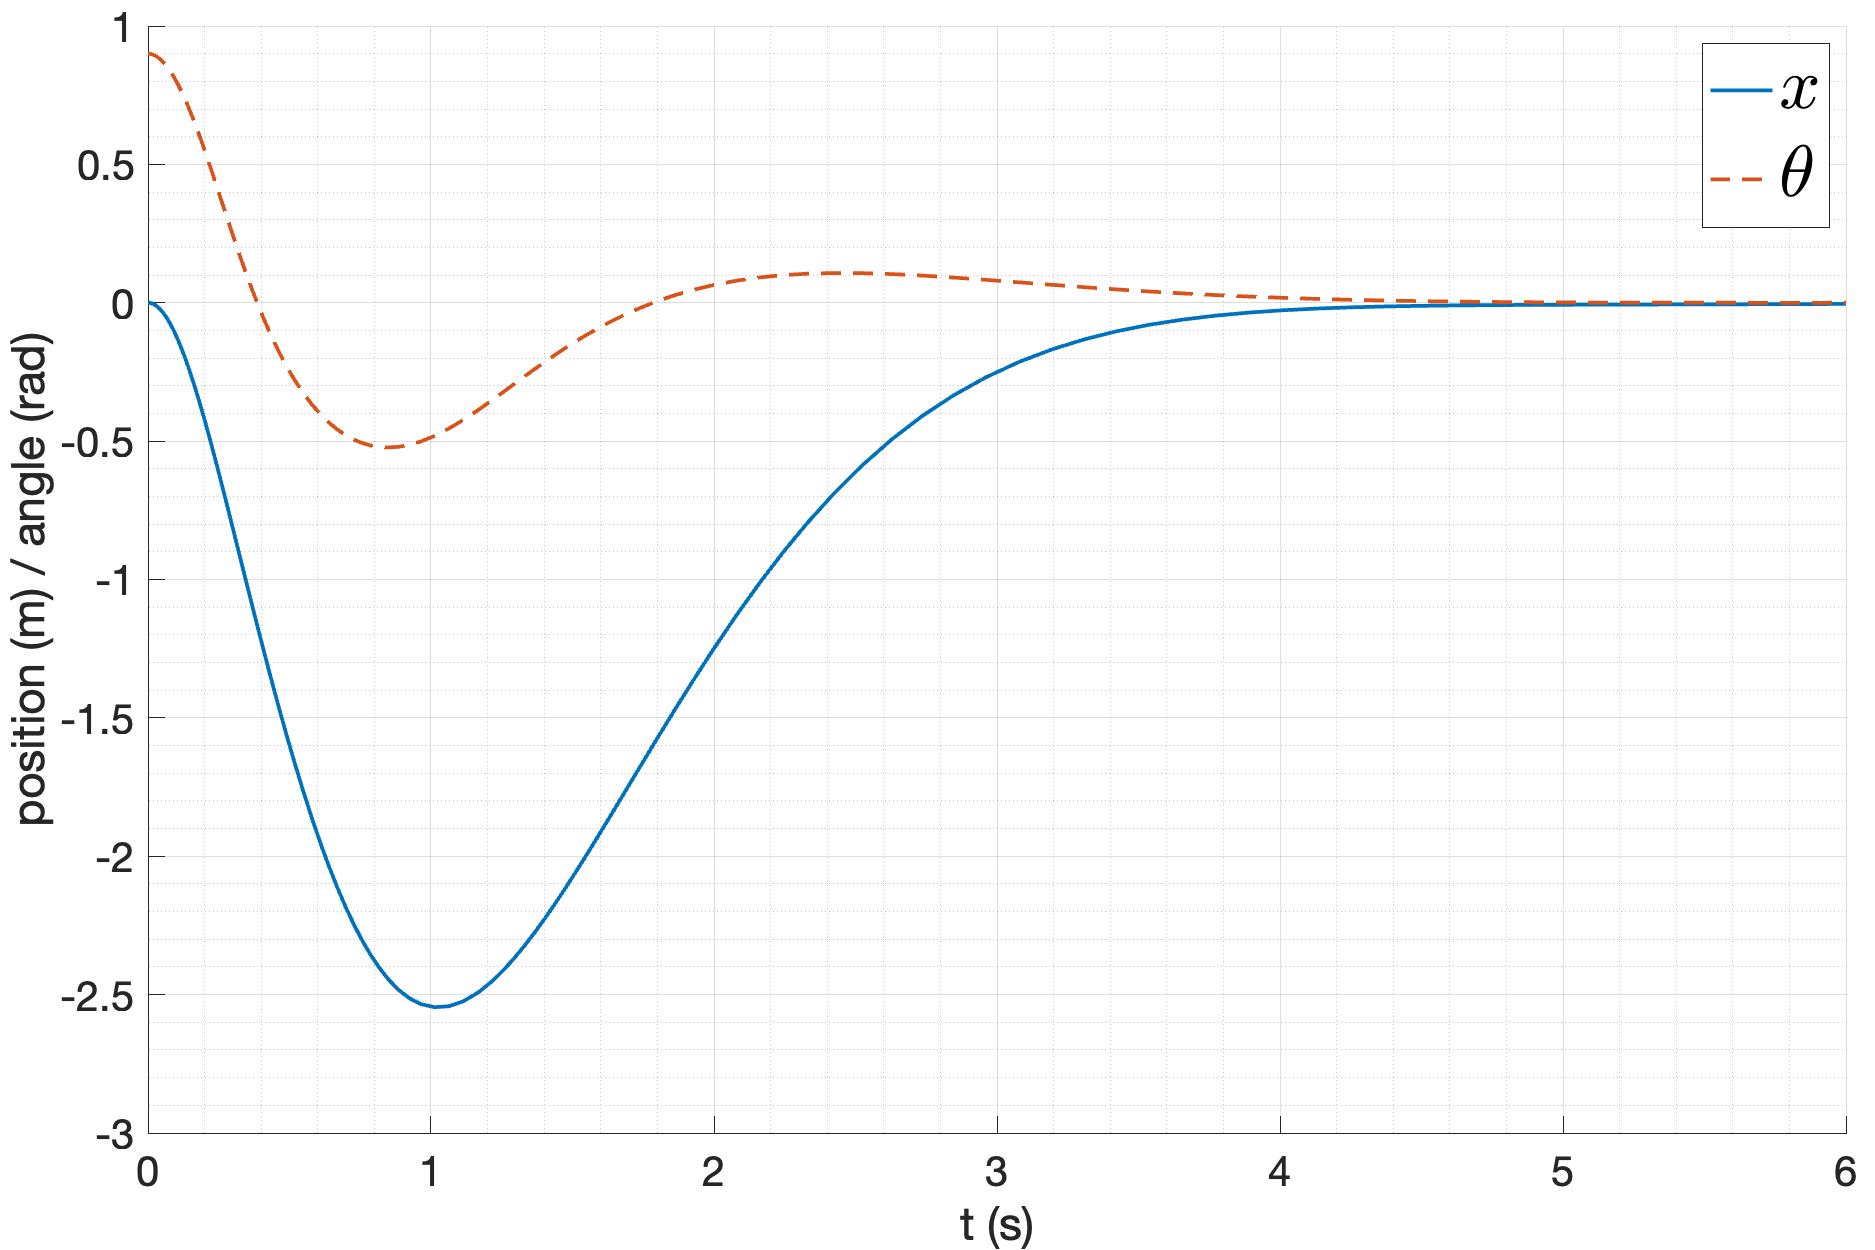
\includegraphics[width=\textwidth]{media/plots/modal_control/out_3.png}
        \caption{$\theta_0 = 0.9$}
    \end{subfigure}
    \begin{subfigure}[b]{0.45\textwidth}
        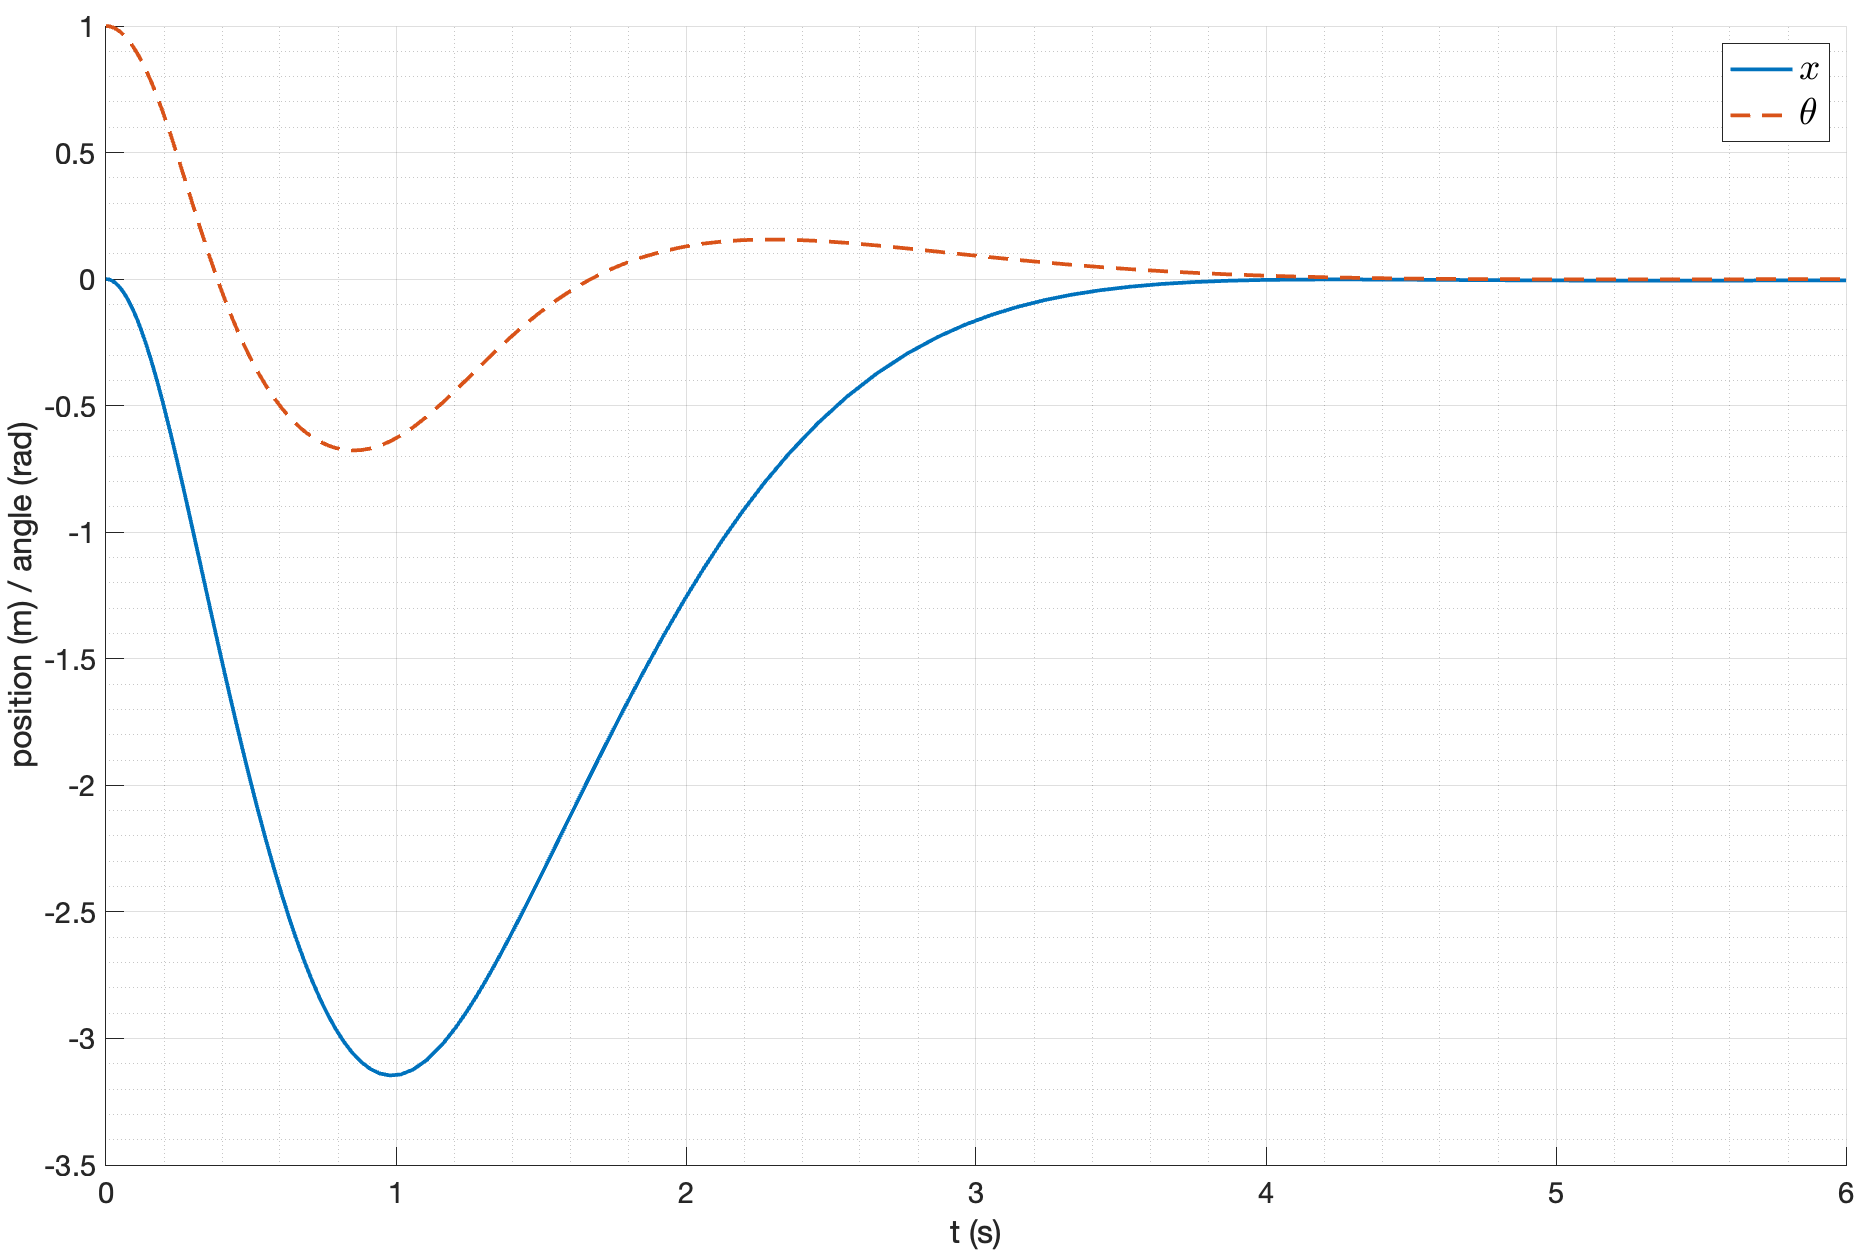
\includegraphics[width=\textwidth]{media/plots/modal_control/out_4.png}
        \caption{$\theta_0 = 1.0$}
    \end{subfigure}
    \begin{subfigure}[b]{0.45\textwidth}
        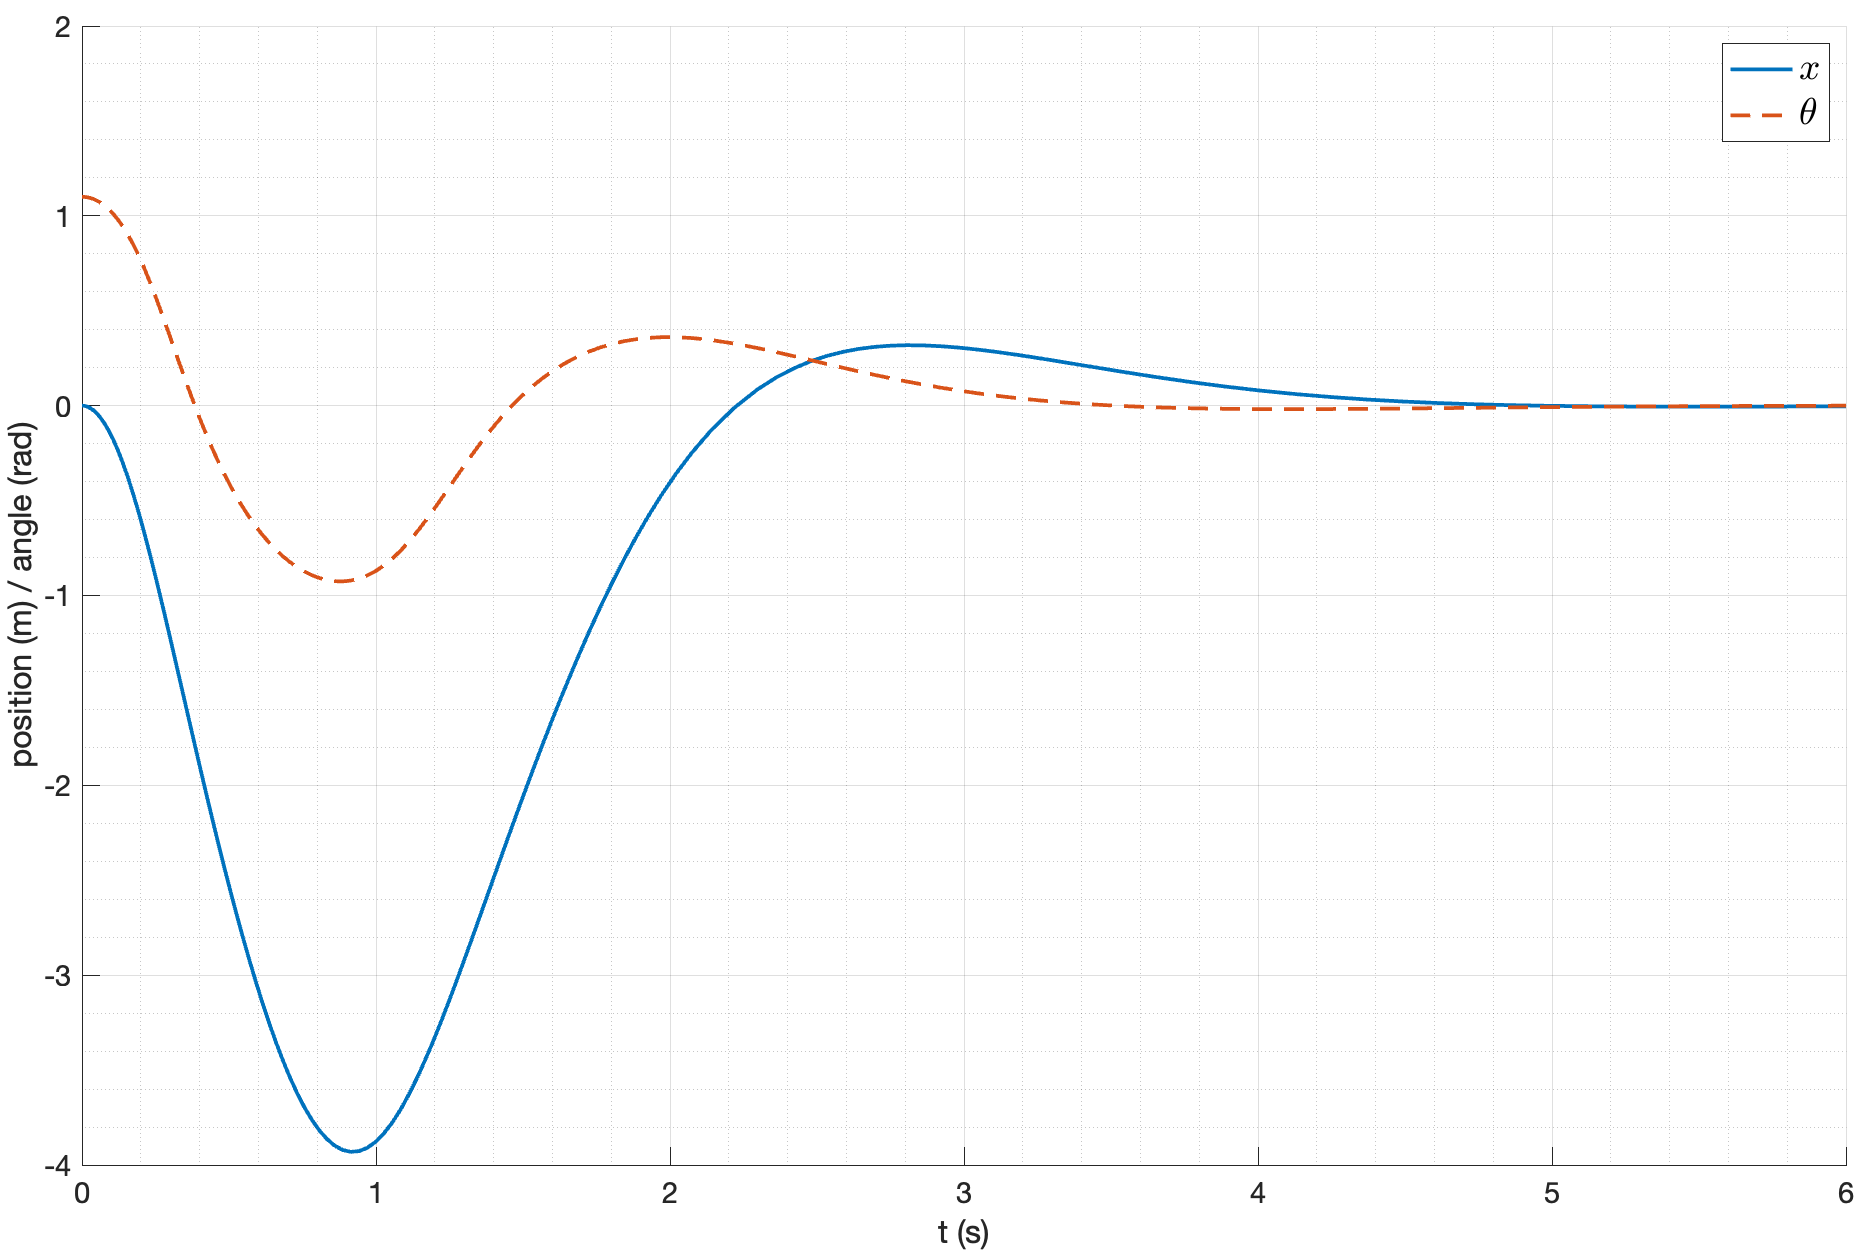
\includegraphics[width=\textwidth]{media/plots/modal_control/out_5.png}
        \caption{$\theta_0 = 1.1$}
    \end{subfigure}
    \begin{subfigure}[b]{0.45\textwidth}
        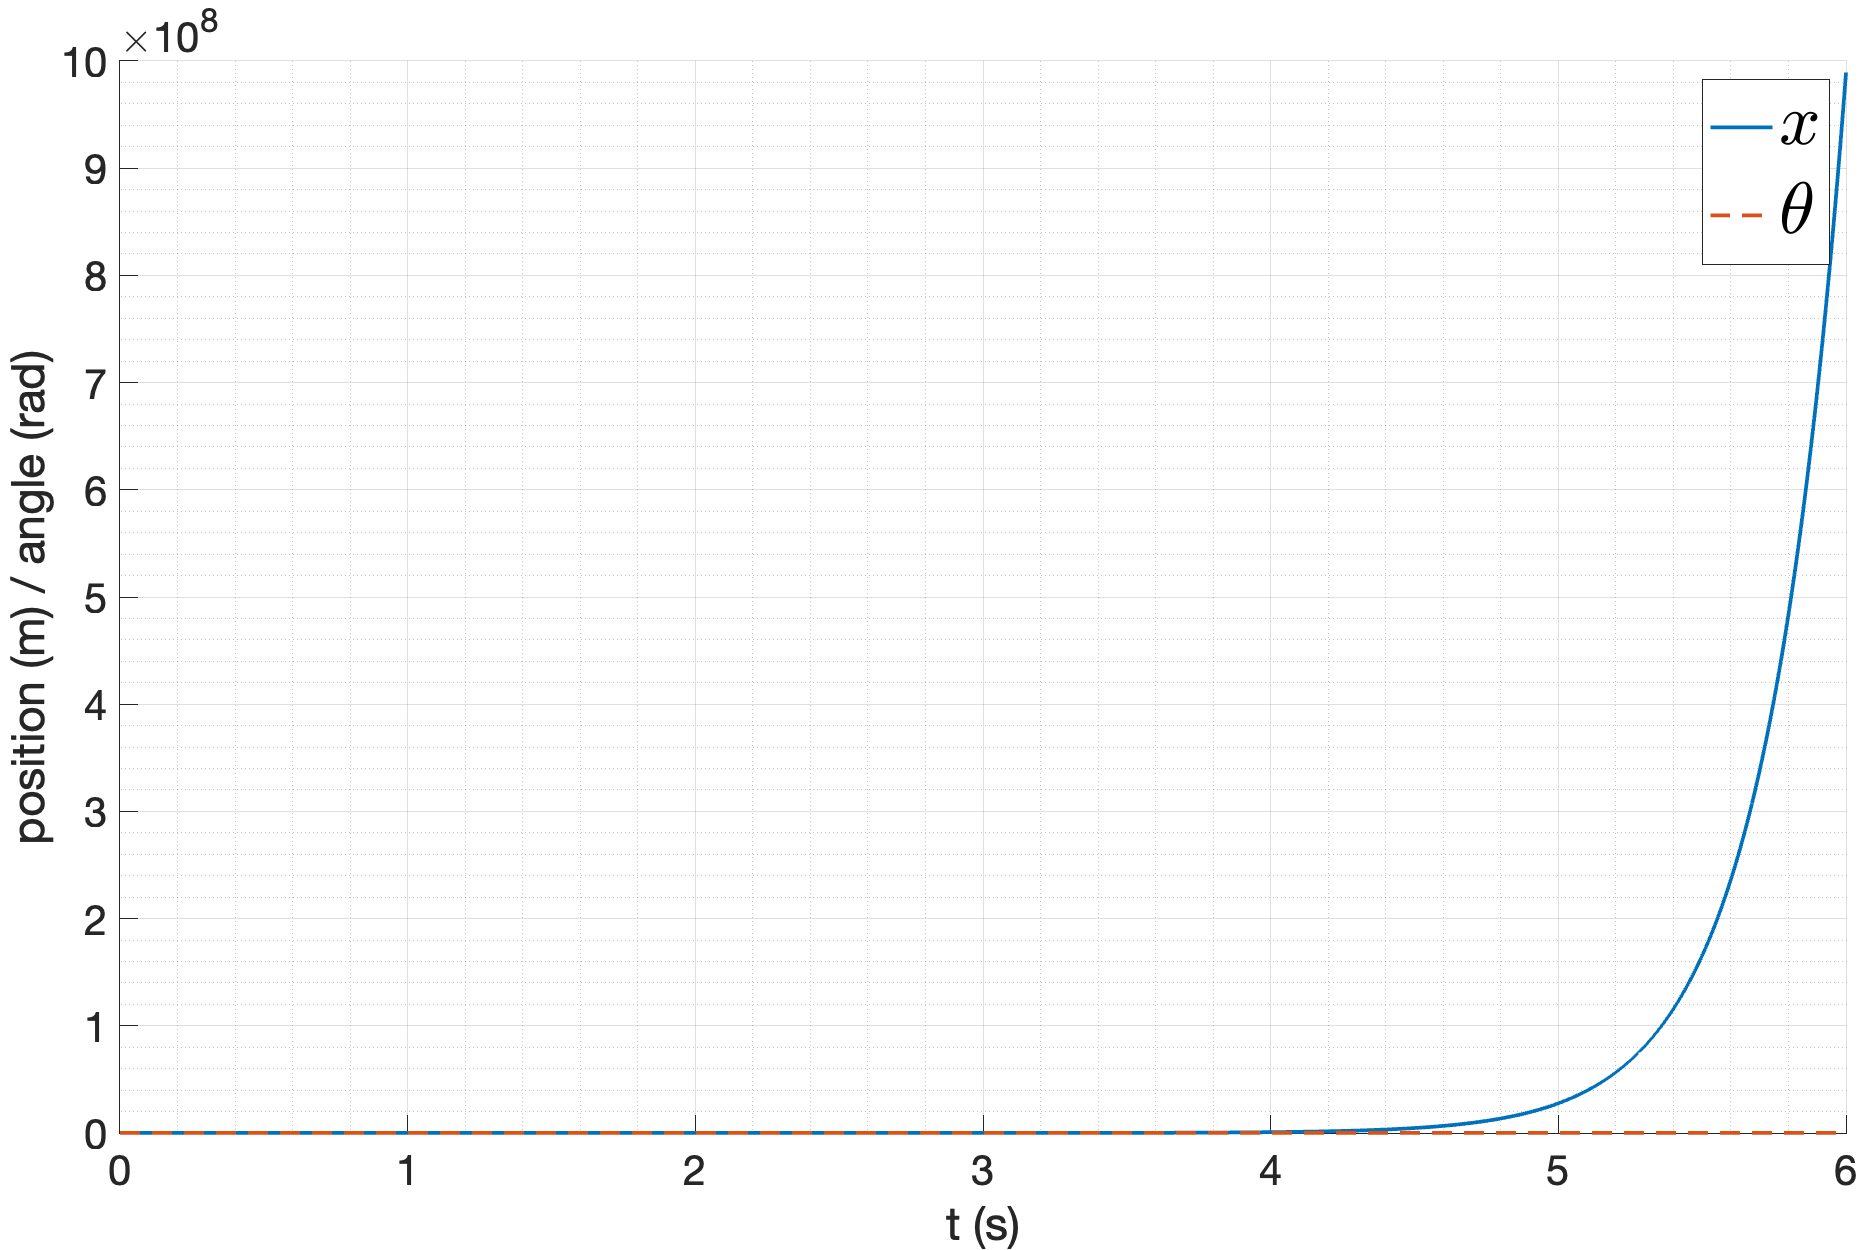
\includegraphics[width=\textwidth]{media/plots/modal_control/out_6.png}
        \caption{$\theta_0 = 1.2$}
    \end{subfigure}
    \caption{Модальное управление нелинейной модели системы}
    \label{fig:modal_control_initials}
\end{figure}
Видно, что при начальном угле отклонения маятника вплоть до $\theta_0 = 1.0$ система приходит в
равновесное состояние. При этом время переходного процесса остается приблизительно одинаковым. 
При дальнейшем увеличении угла начального отклонения маятника система не приходит в равновесное состояние, 
это связано с тем, что при больших отклонениях маятника от вертикального положения линейная модель, на основе 
которой был синтезирован регулятор, перестает адекватно описывать поведение системы. Убедиться в этом можно 
посмотрев на график поведения линейной модели системы при начальном угле отклонения $\theta_0 = 1.2$ (рисунок \ref{fig:modal_control_linear_out_6}).
\begin{figure}[ht!]
    \centering
    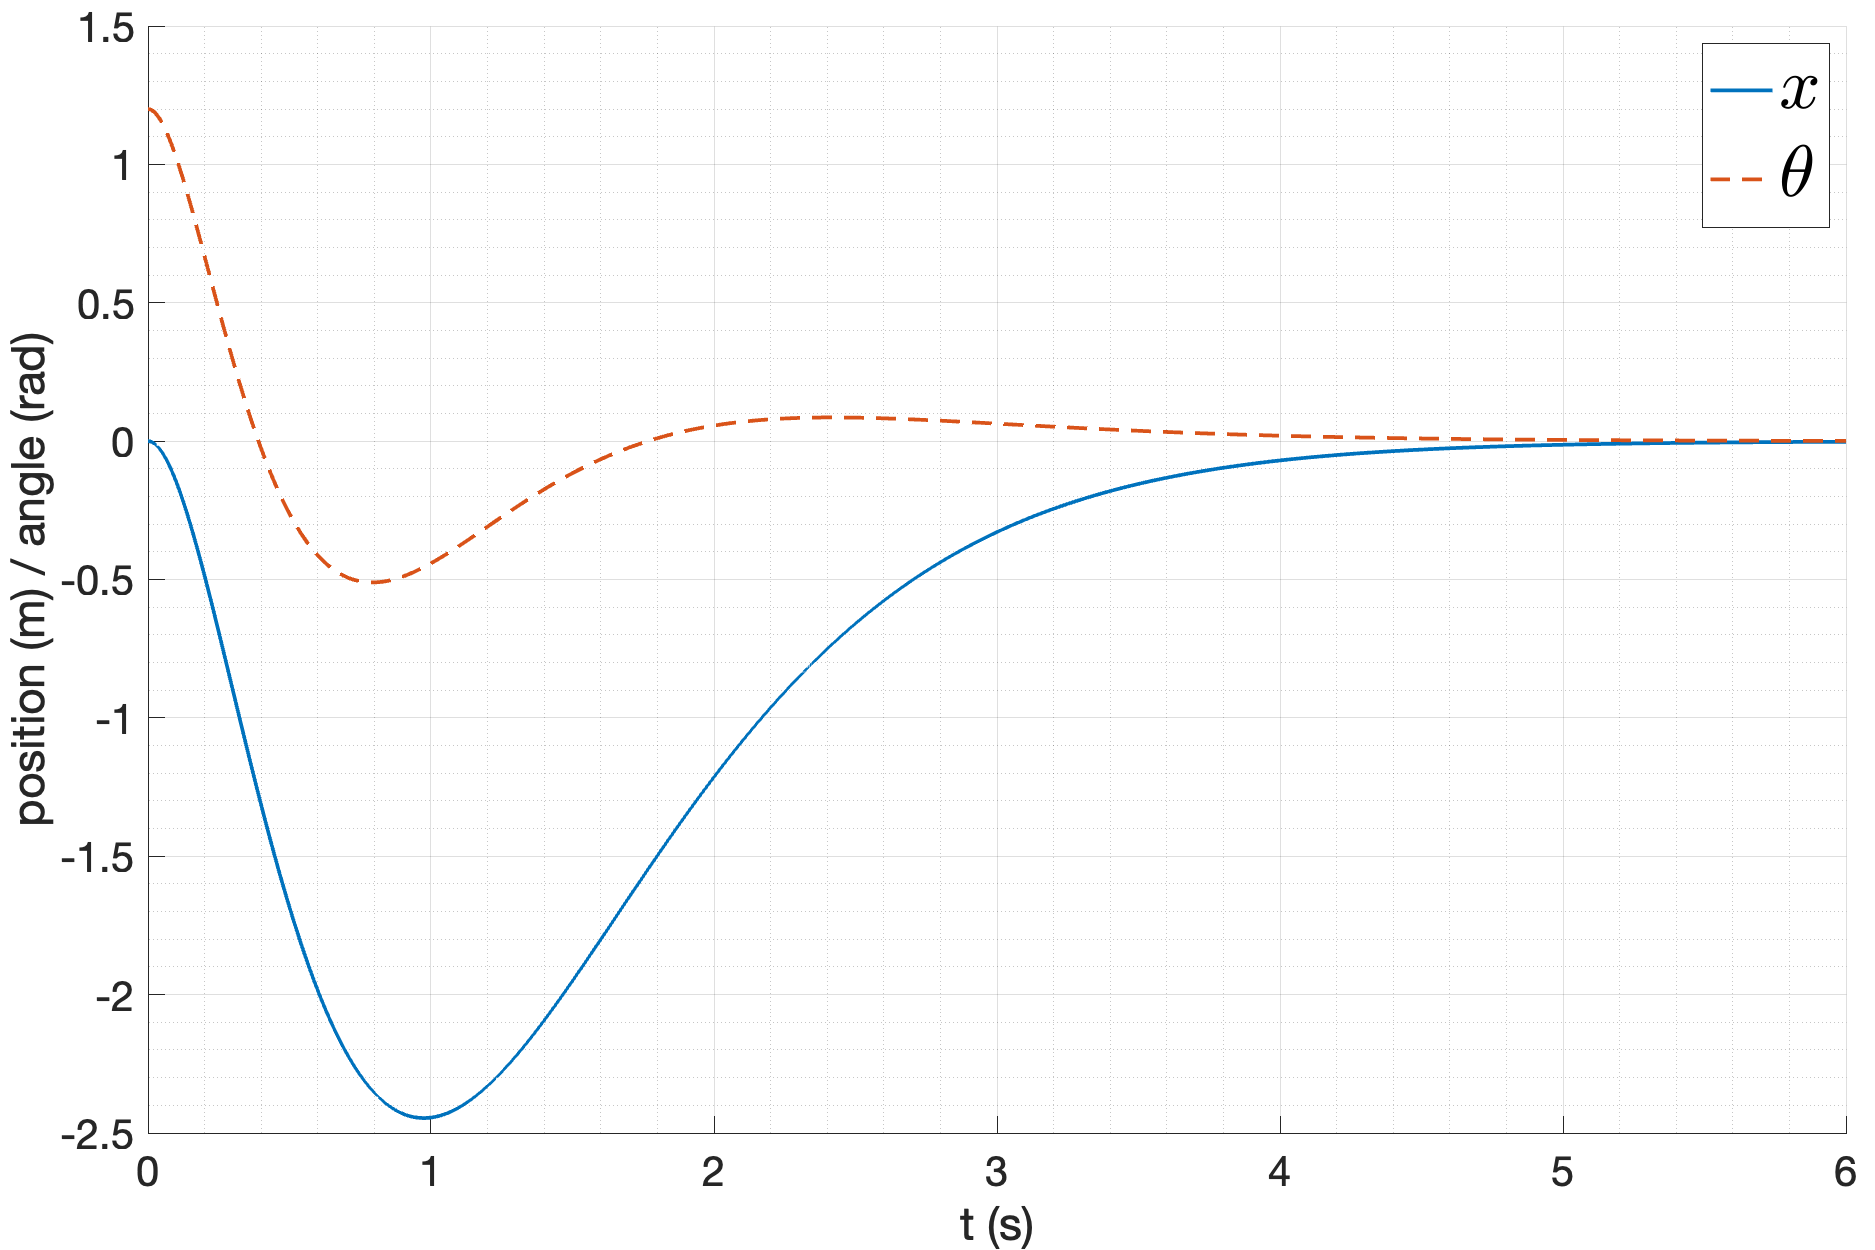
\includegraphics[width=\textwidth]{media/plots/modal_control/linear_out_6.png}
    \caption{Результаты моделирования линейной модели системы с модальным регулятором при $\theta_0 = 1.2$}
    \label{fig:modal_control_linear_out_6}
\end{figure}
\FloatBarrier
Видно, что линейная модель система приходит в равновесное состояния, в отличие от нелинейной модели.

\subsection{Исследование переходного процесса}
Будем рассматривать переходный процесс и управляющее воздействие при различных собственных числах замкнутой регулятором системы. 
В качестве начальных условий возьмем $\theta_0 = 0.3$. Для начала, рассмотрим регуляторы, обеспечивающие спектр 
замкнутой системы вида $\sigma_k = \begin{bmatrix}k & k & k & k\end{bmatrix}$, где $k \in \begin{bmatrix}-4, -6, -8, -10\end{bmatrix}$. 
Результаты моделирования приведены на рисунках \ref{fig:modal_controlers_1_out} -- \ref{fig:modal_controlers_4_u}.

\begin{figure}[ht!]
    \centering
    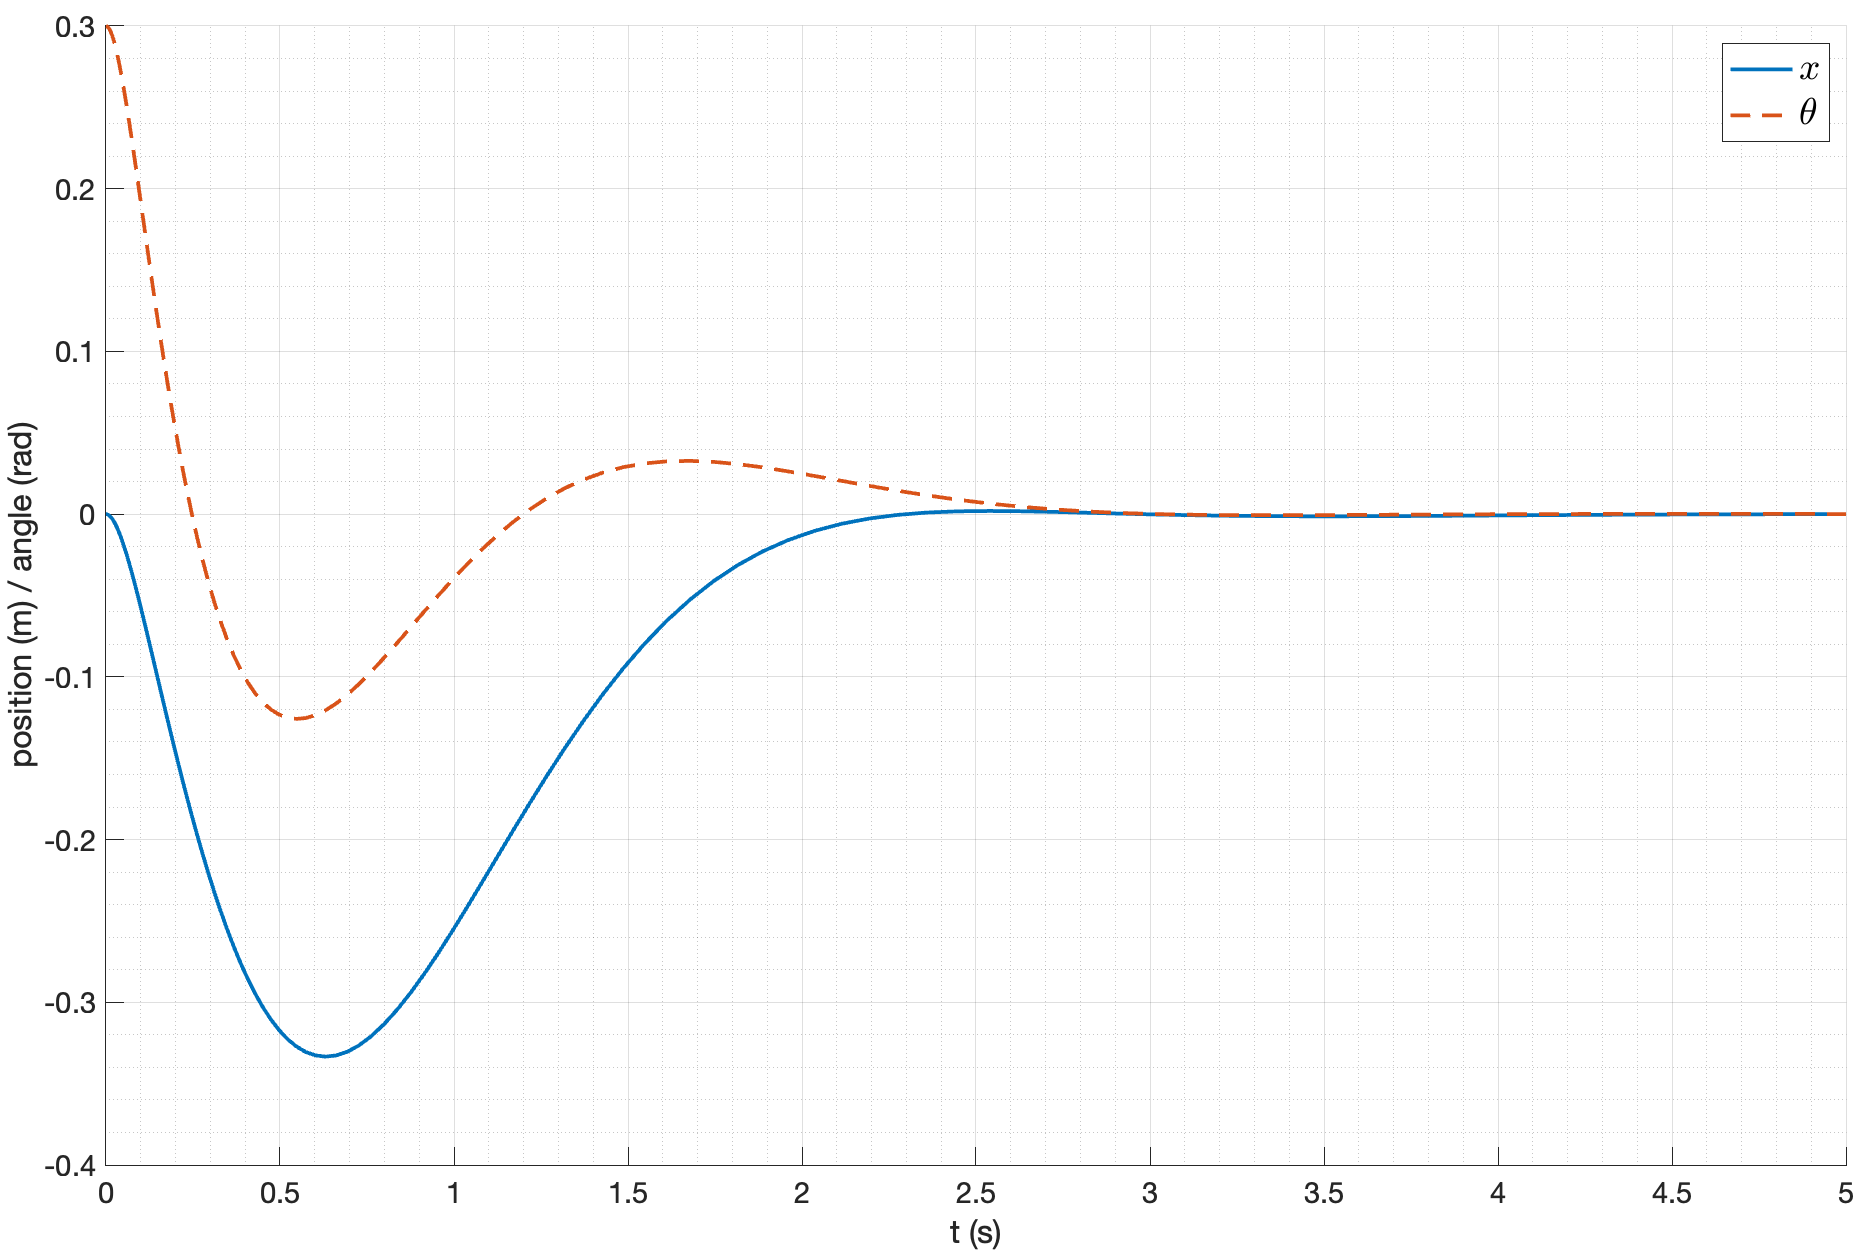
\includegraphics[width=0.8\textwidth]{media/plots/modal_controllers/out_1.png}
    \caption{Результаты моделирования нелинейной модели системы с модальным регулятором при $k = -4$}
    \label{fig:modal_controlers_1_out}
\end{figure}
\begin{figure}[ht!]
    \centering
    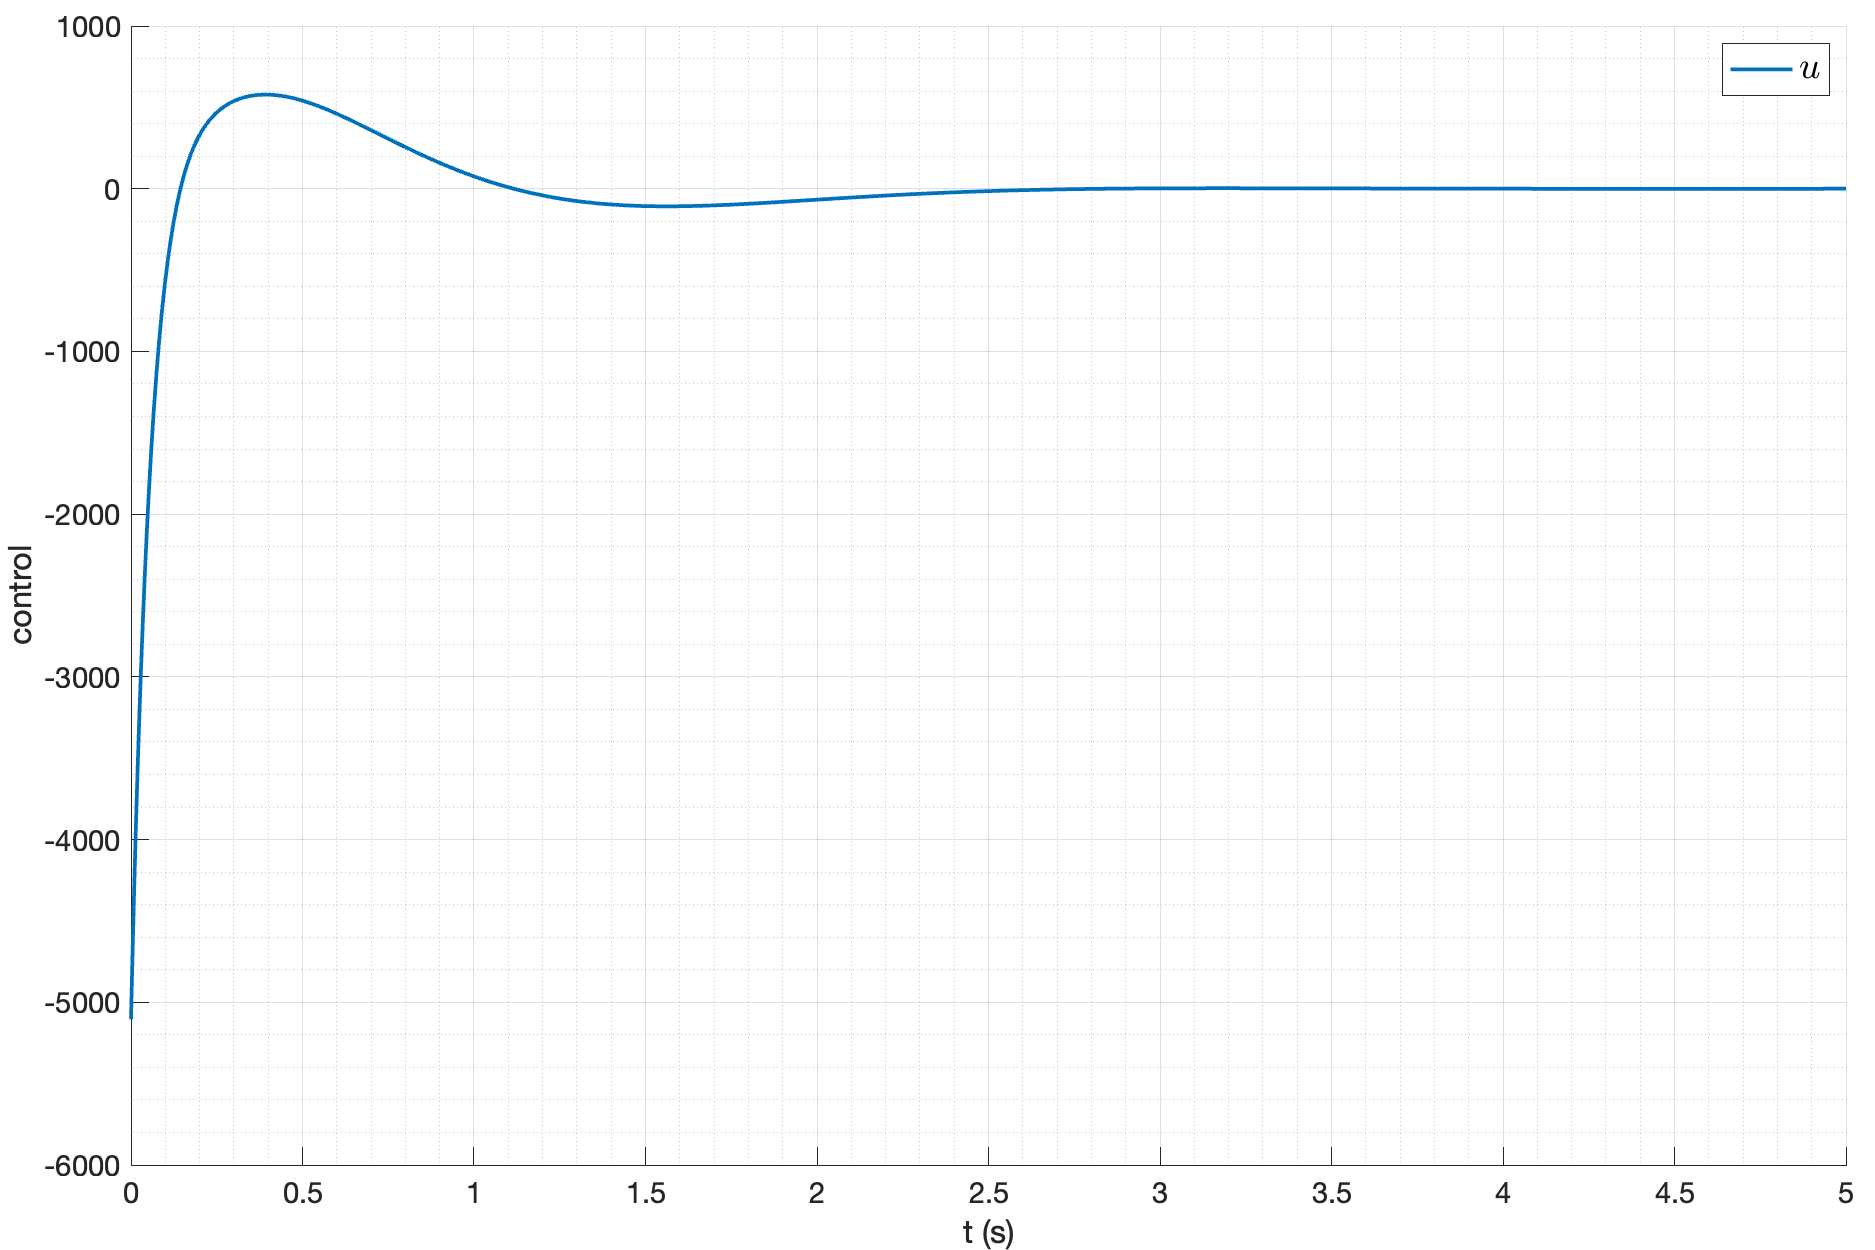
\includegraphics[width=0.8\textwidth]{media/plots/modal_controllers/u_1.png}
    \caption{Управляющее воздействие нелинейной модели системы с модальным регулятором при $k = -4$}
    \label{fig:modal_controlers_1_u}
\end{figure}
\begin{figure}[ht!]
    \centering
    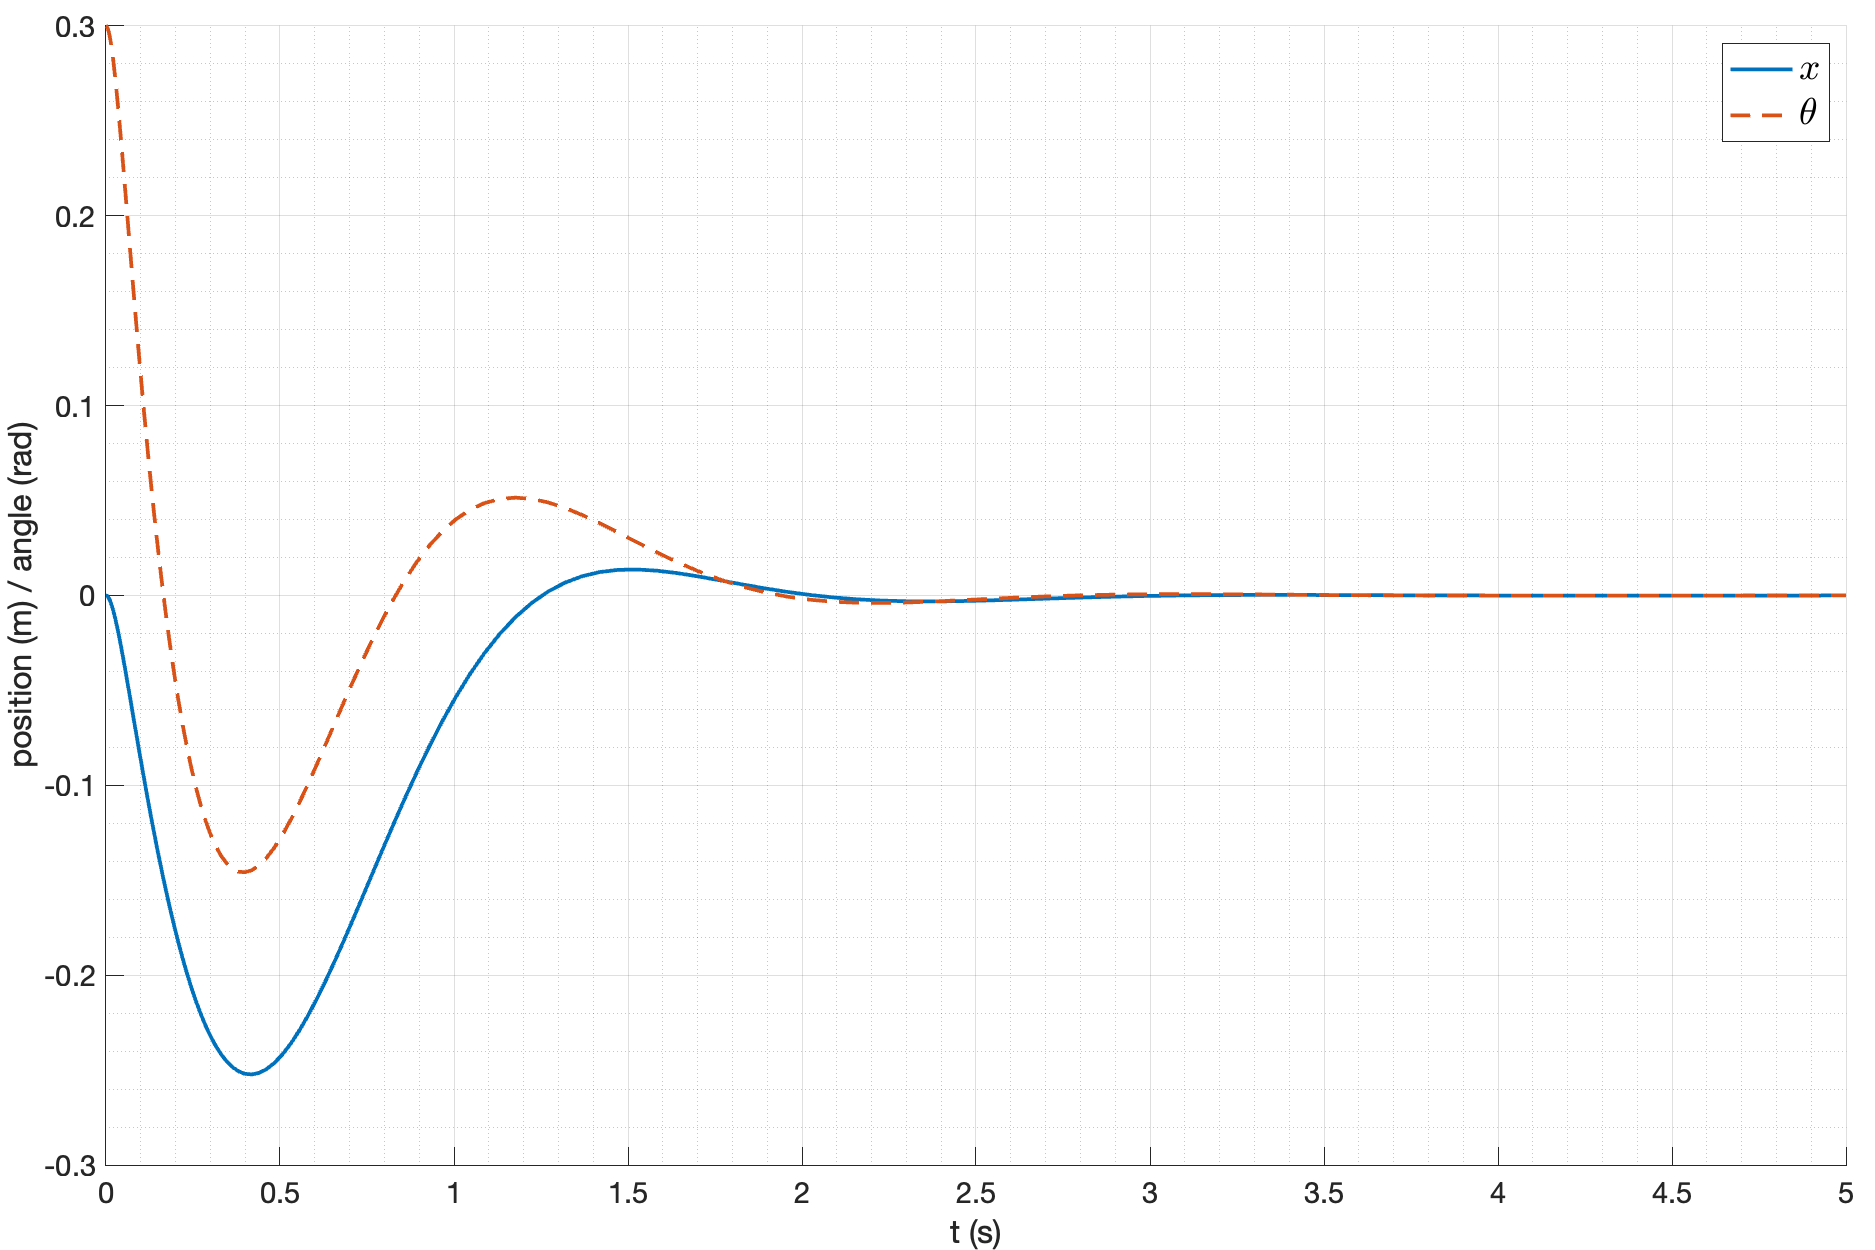
\includegraphics[width=0.8\textwidth]{media/plots/modal_controllers/out_2.png}
    \caption{Результаты моделирования нелинейной модели системы с модальным регулятором при $k = -6$}
    \label{fig:modal_controlers_2_out}
\end{figure}
\begin{figure}[ht!]
    \centering
    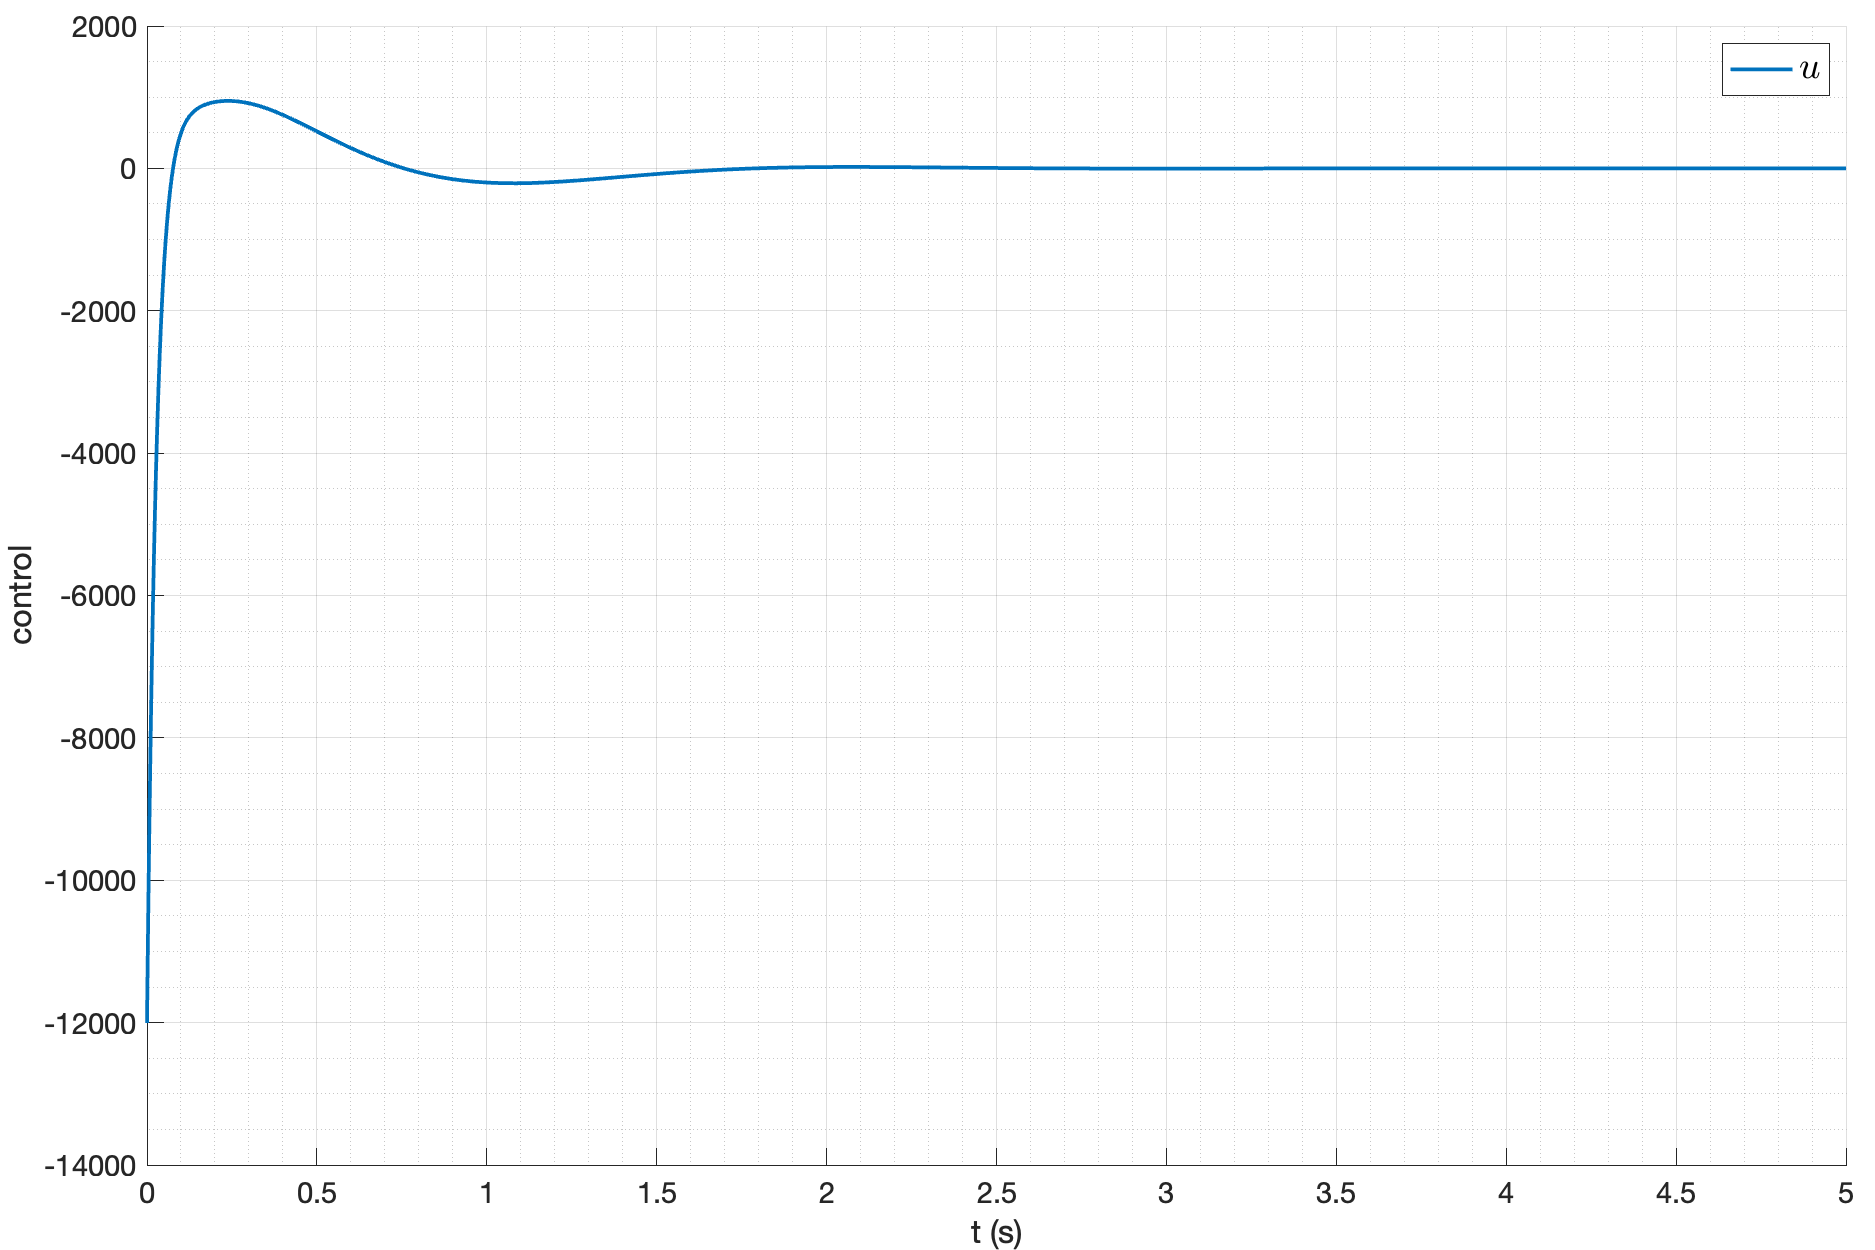
\includegraphics[width=0.8\textwidth]{media/plots/modal_controllers/u_2.png}
    \caption{Управляющее воздействие нелинейной модели системы с модальным регулятором при $k = -6$}
    \label{fig:modal_controlers_2_u}
\end{figure}
\begin{figure}[ht!]
    \centering
    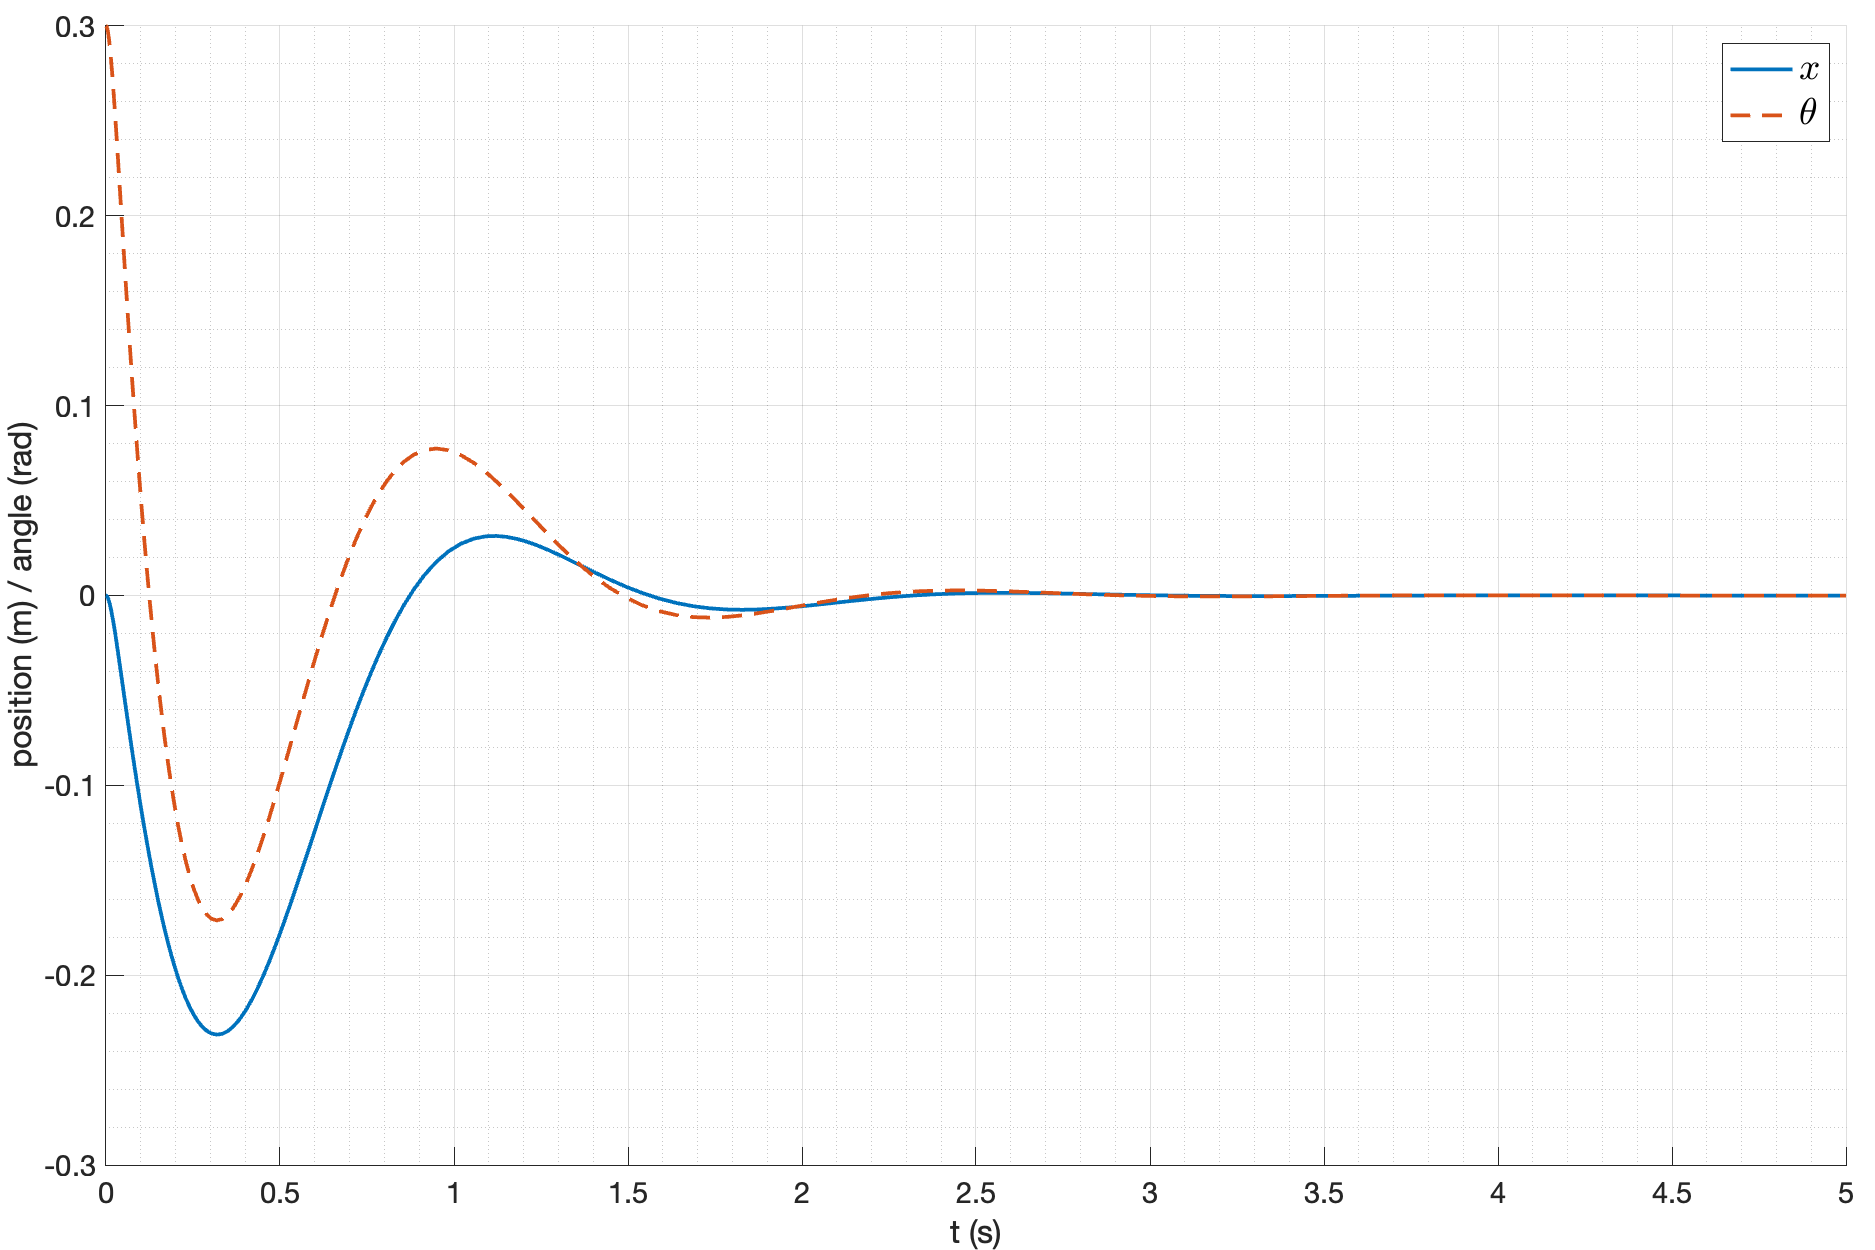
\includegraphics[width=0.8\textwidth]{media/plots/modal_controllers/out_3.png}
    \caption{Результаты моделирования нелинейной модели системы с модальным регулятором при $k = -8$}
    \label{fig:modal_controlers_3_out}
\end{figure}
\begin{figure}[ht!]
    \centering
    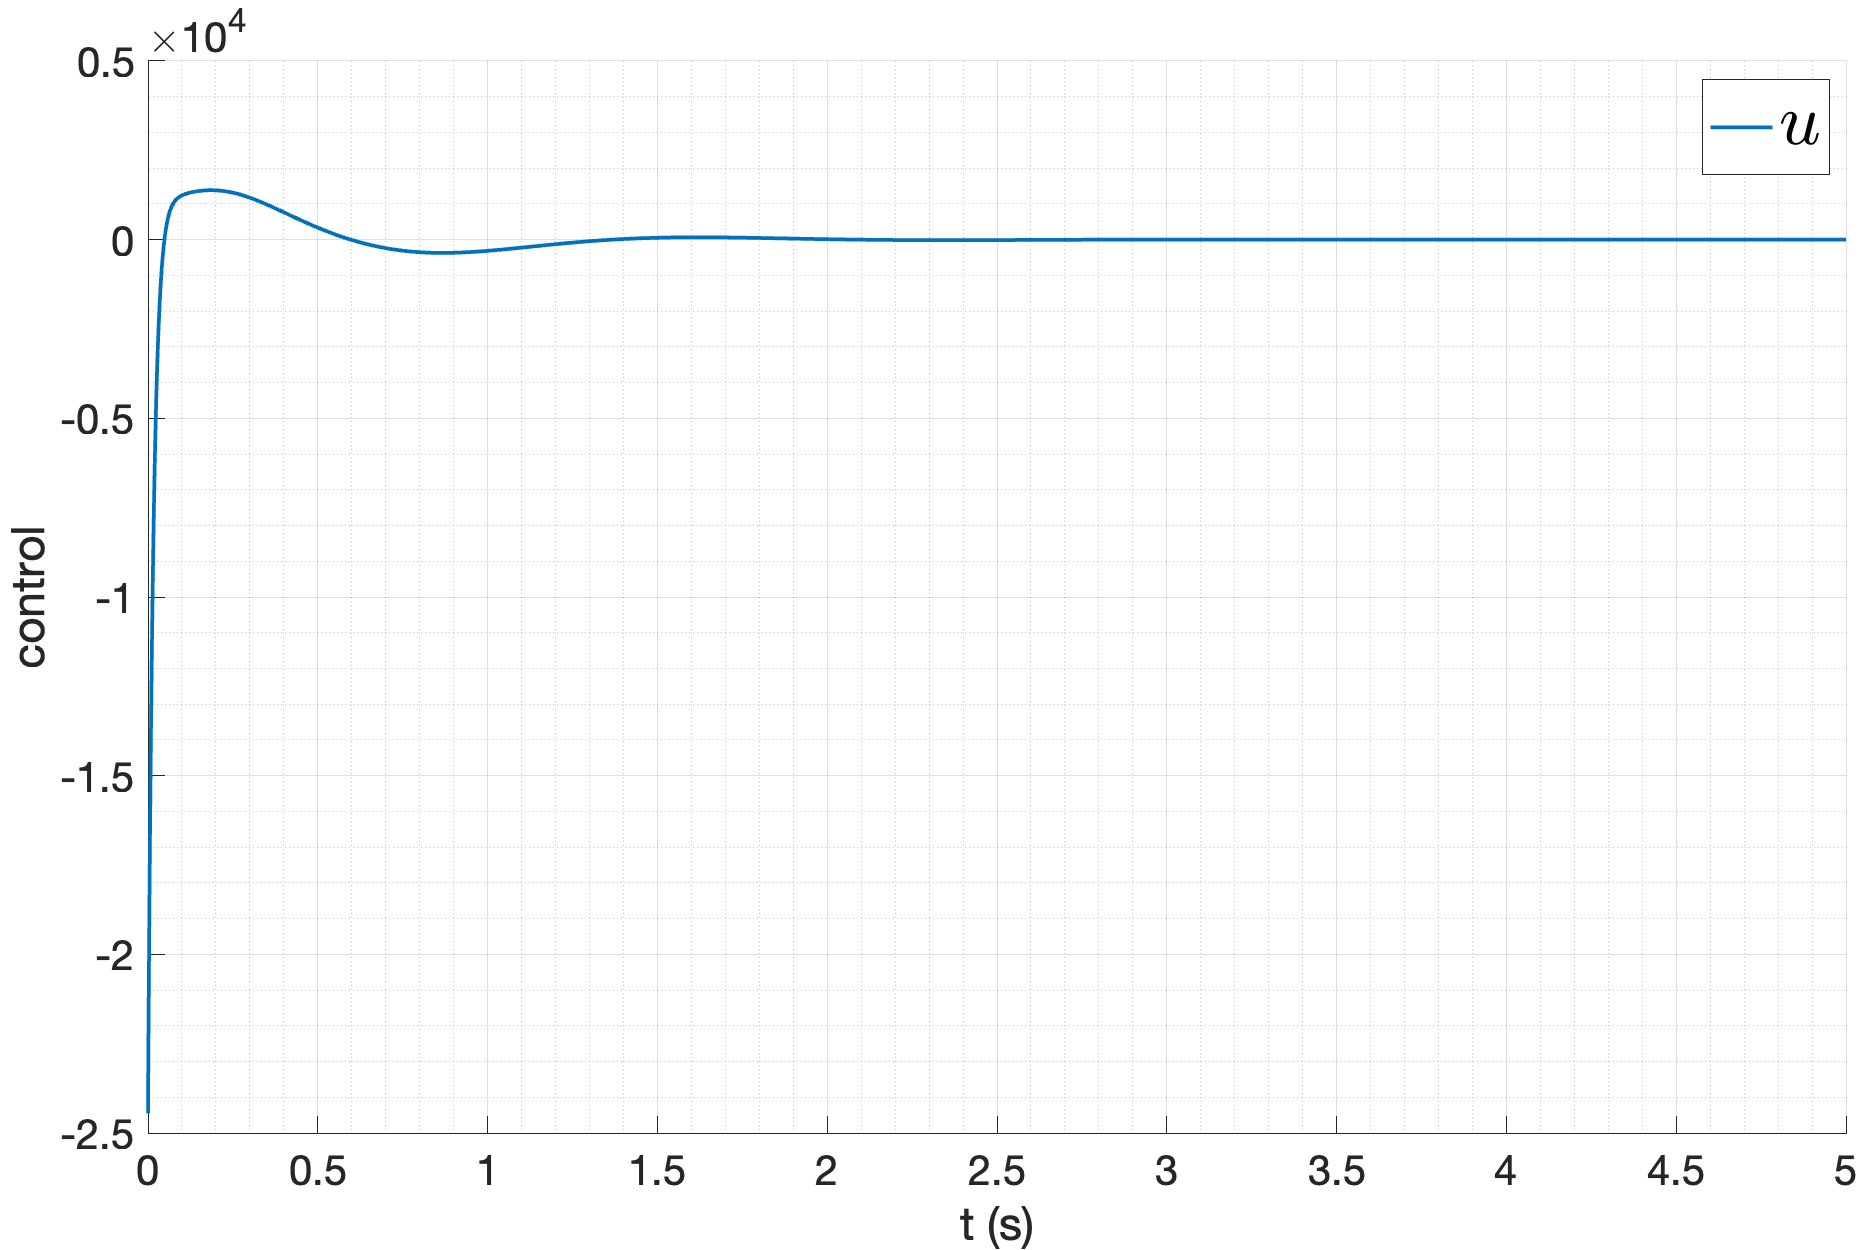
\includegraphics[width=0.8\textwidth]{media/plots/modal_controllers/u_3.png}
    \caption{Управляющее воздействие нелинейной модели системы с модальным регулятором при $k = -8$}
    \label{fig:modal_controlers_3_u}
\end{figure}
\begin{figure}[ht!]
    \centering
    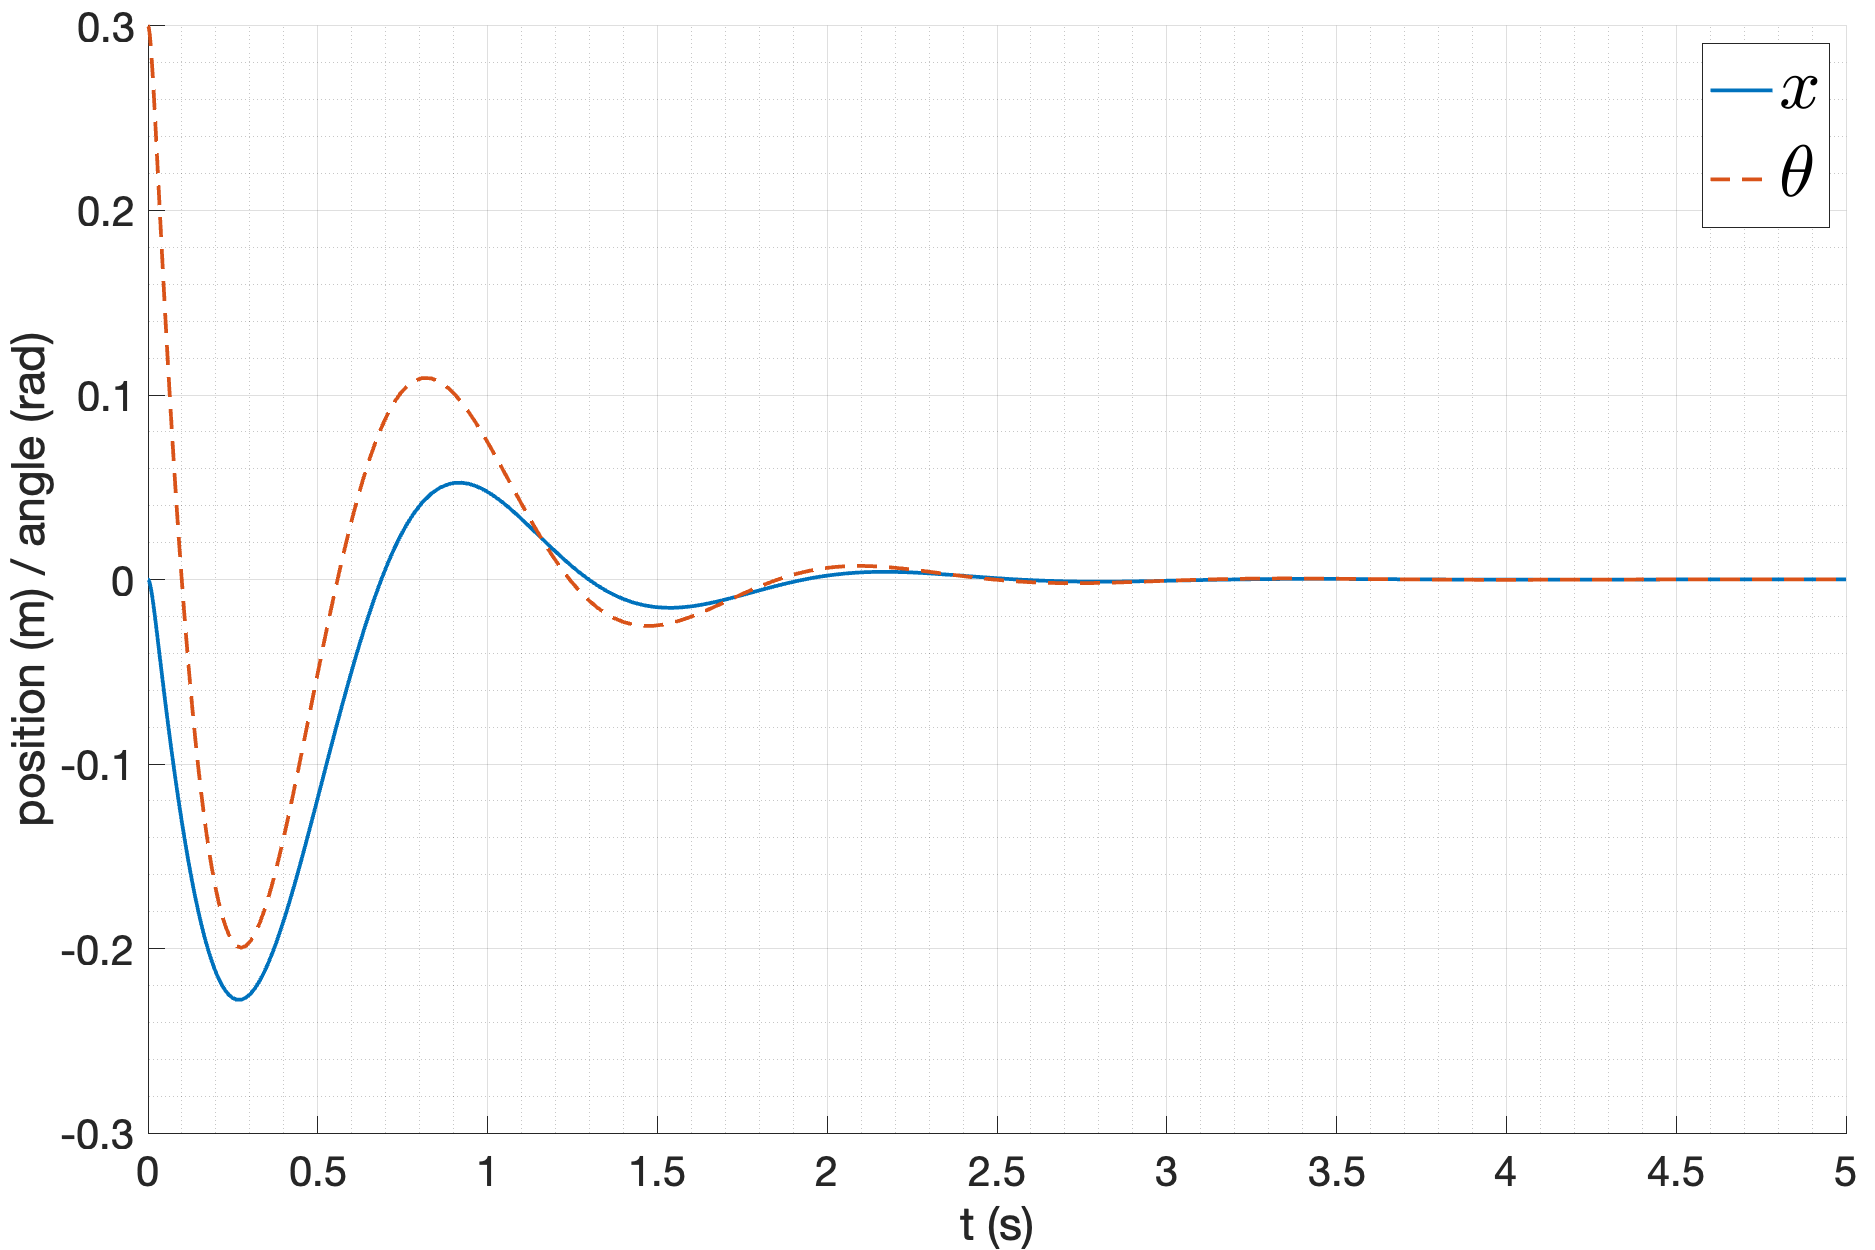
\includegraphics[width=0.8\textwidth]{media/plots/modal_controllers/out_4.png}
    \caption{Результаты моделирования нелинейной модели системы с модальным регулятором при $k = -10$}
    \label{fig:modal_controlers_4_out}
\end{figure}
\begin{figure}[ht!]
    \centering
    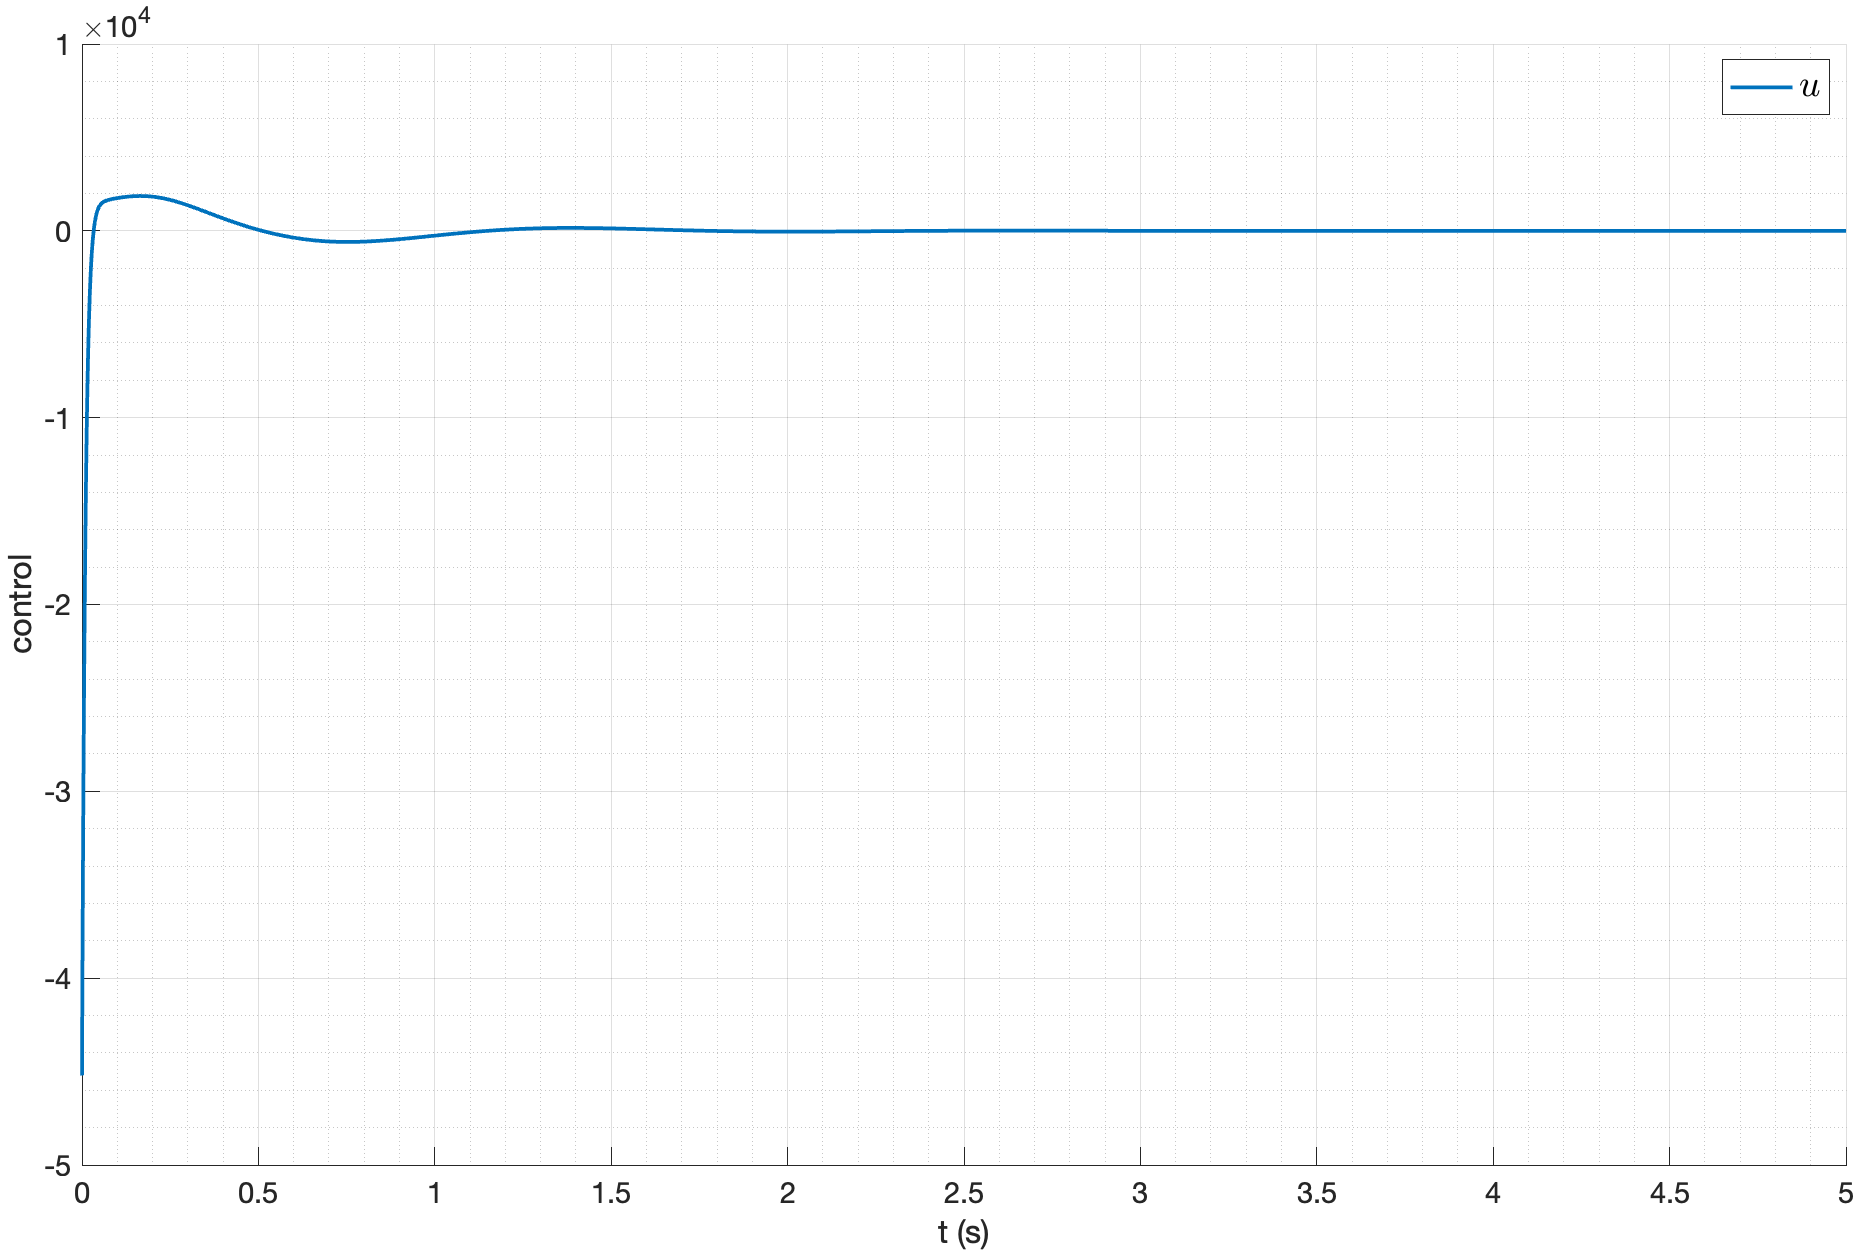
\includegraphics[width=0.8\textwidth]{media/plots/modal_controllers/u_4.png}
    \caption{Управляющее воздействие нелинейной модели системы с модальным регулятором при $k = -10$}
    \label{fig:modal_controlers_4_u}
\end{figure}
Можно заметить, что при увеличении модуля собственных чисел замкнутой системы, время переходного процесса
сокращается, а перегулирование отклонения маятника увеличивается, максимальный модуль управляющего воздействия 
тоже увеличивается с увеличением модуля собственных чисел. Численные результаты сравнения приведены в таблице \ref{tab:modal_control_cmp}. 

\begin{table}[ht!]
    \centering
    \begin{tabular}{|c|c|c|c|c|}
        \hline
        $k$ & $t_{\text{set}}$, с & $M_{\theta}$ & $M_{x}$ & $\max{|u|}$ \\
        \hline
        -4 & 2.9 & 0.11 & 0.34 & 5100 \\
        \hline
        -6 & 2.7 & 0.16 & 0.26 & 12000 \\
        \hline
        -8 & 2.5 & 0.18 & 0.24 & 24000 \\
        \hline
        -10 & 1.4 & 0.2 & 0.23 & 44000 \\
        \hline
    \end{tabular}
    \caption{Сравнение регуляторов с различными собственными числами замкнутой системы}
    \label{tab:modal_control_cmp}
\end{table}

Можно заметить, что перегулирование координаты тележки остается практически одинаковым, 
что связано с тем, что угол маятника зависит от скорости и ускорения тележки, а не от ее положения. 

\FloatBarrier
Дополнительно посмотрим на случай замкнутой системы, имеющий спектр $\begin{bmatrix}-0.5 & -0.5 & -4 &- 4\end{bmatrix}$
и сравним ее с системой, имеющей спектр $\begin{bmatrix}-4 & -4 & -4 &- 4\end{bmatrix}$, рассмотренной на рисунке \ref{fig:modal_controlers_1_out}.
Графики результатов моделирования приведены на рисунке \ref{fig:modal_controlers_5_out} -- \ref{fig:modal_controlers_5_u}. 
\begin{figure}[ht!]
    \centering
    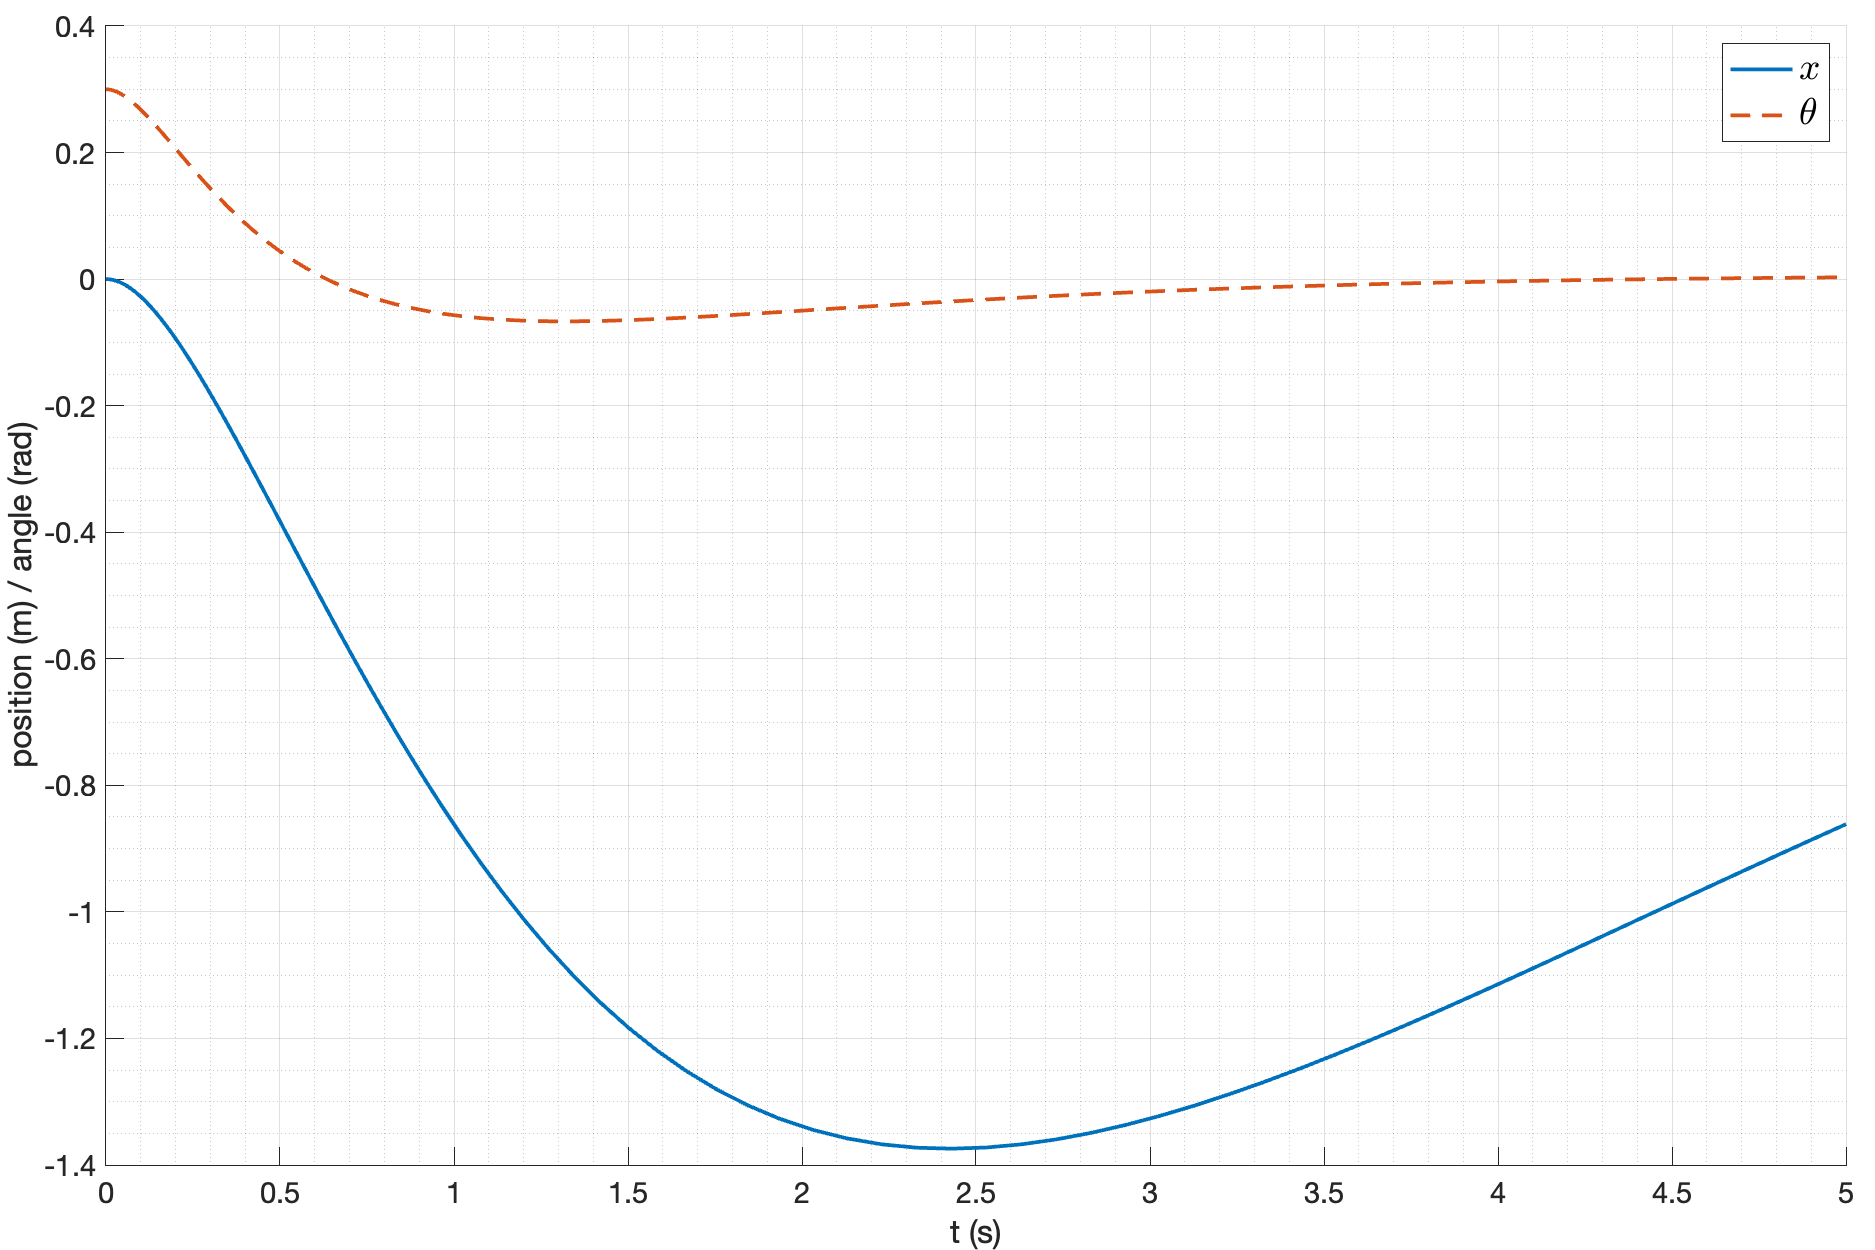
\includegraphics[width=0.8\textwidth]{media/plots/modal_controllers/out_5.png}
    \caption{Результаты моделирования нелинейной модели системы со спектром $\begin{bmatrix}-0.5 & -0.5 & -4 &- 4\end{bmatrix}$}
    \label{fig:modal_controlers_5_out}
\end{figure}
\begin{figure}[ht!]
    \centering
    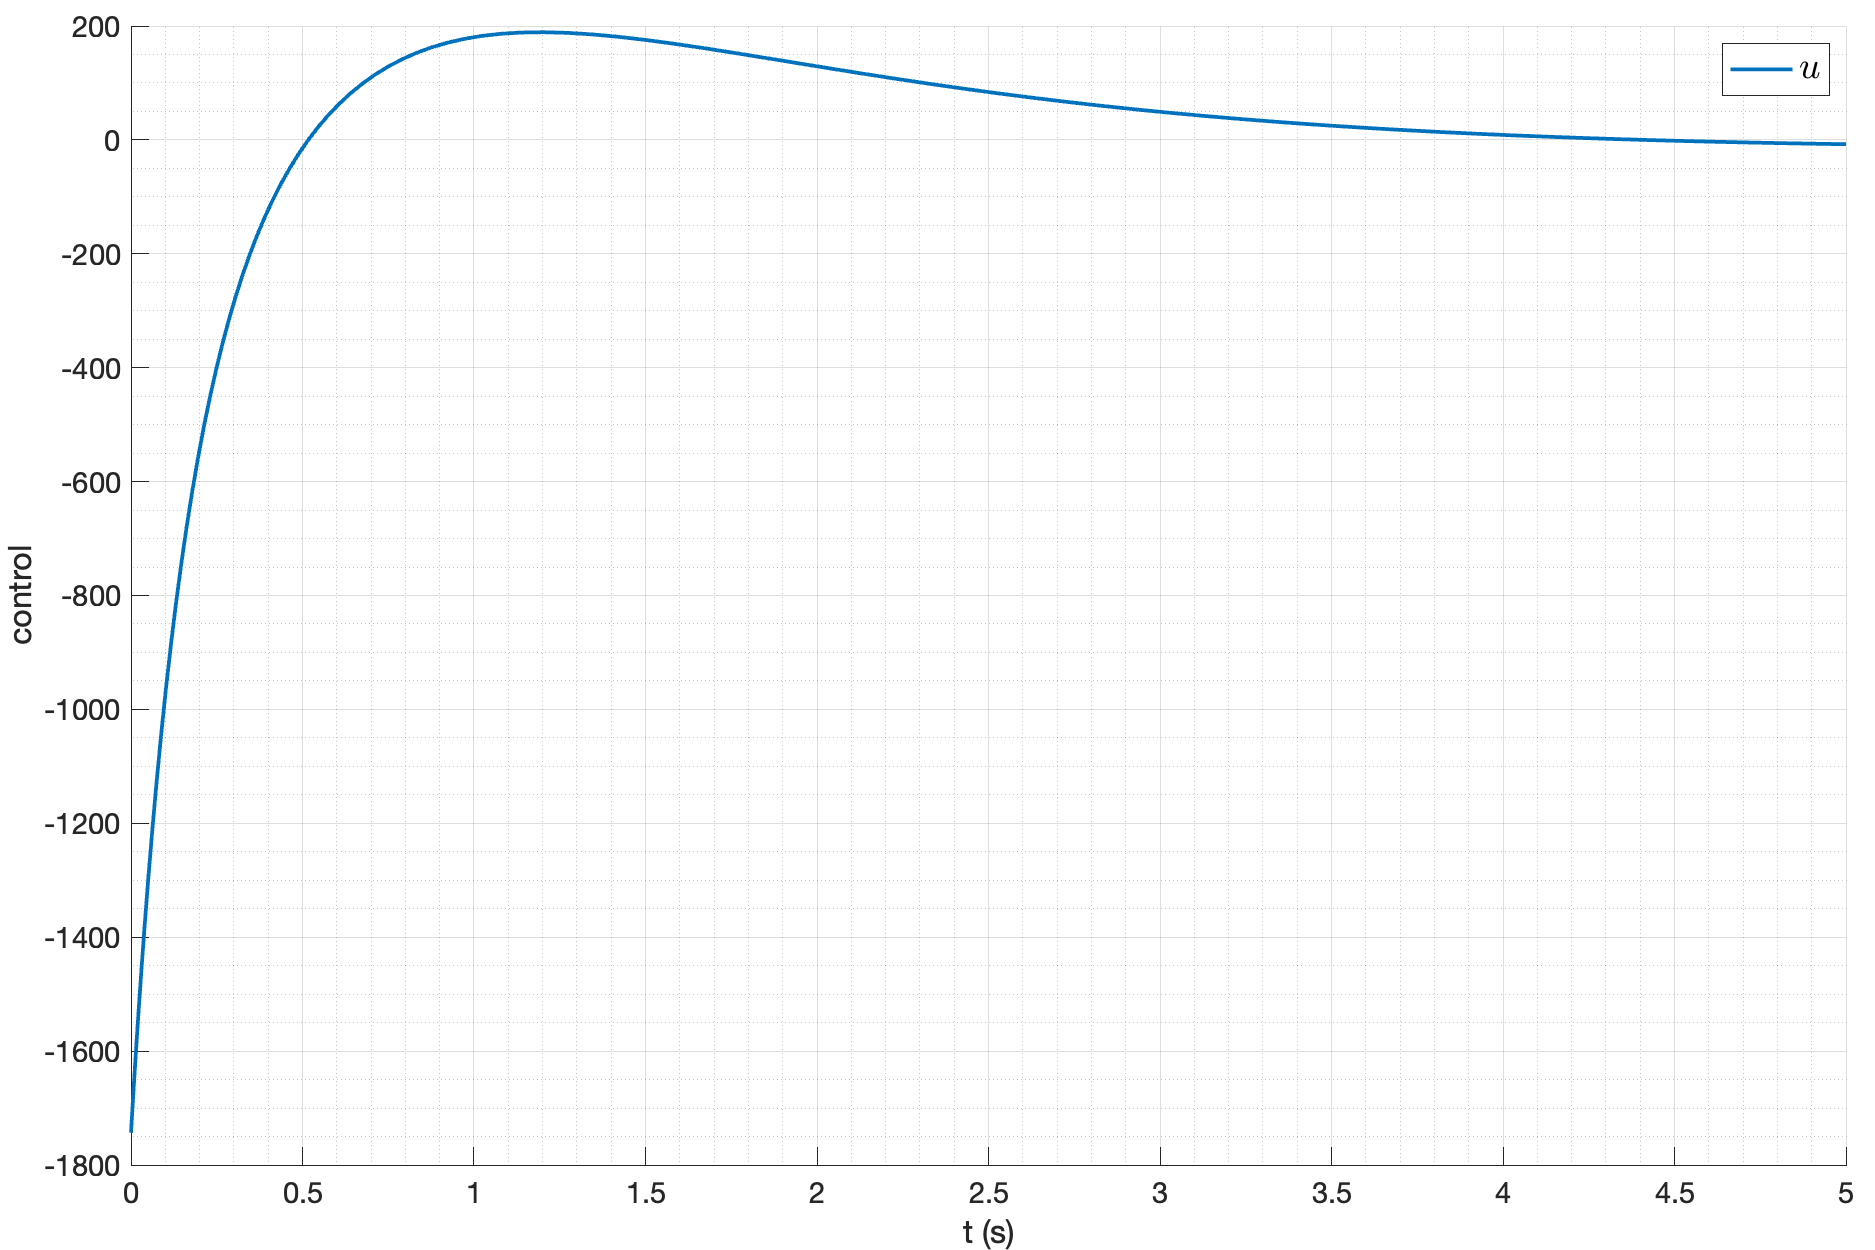
\includegraphics[width=0.8\textwidth]{media/plots/modal_controllers/u_5.png}
    \caption{Управляющее воздействие нелинейной модели системы со спектром $\begin{bmatrix}-0.5 & -0.5 & -4 &- 4\end{bmatrix}$}
    \label{fig:modal_controlers_5_u}
\end{figure}
\FloatBarrier
Видно, что при уменьшении первых двух собственных чисел замкнутой системы, время переходного процесса для 
координаты тележки сильно увеличивается, а для угла отклонения маятника практически не меняется, при этом 
управление тоже становится меньше. При уменьшении первых двух собственных чисел произошло влияние на первые 
два собственные вектора системы (\ref{eq:eigenvectors}), которые, в свою очередь, влияют на 
линейное положение тележки, но не на угол отклонения маятника. Таким образом, можно сделать вывод, что 
с использованием модального управления можно влиять на динамику системы \textit{по отдельности}, изменяя 
собственные числа для каждого из собственных векторов.

\subsection{Наблюдатель полного порядка}
Рассмотрим наблюдатель полного порядка, основанный на линейной модели системы: 
\begin{equation}
    \begin{cases}
        \dot{\hat{x}} = A\hat{x} + Bu + L(y - C\hat{x})\\
        \hat{y} = C\hat{x}
    \end{cases}
\end{equation}
где $L$ -- матрица коррекции наблюдателя. 

Для синтеза наблюдателя воспользуемся уравнением Сильвестра, решение которого будем находить с помощью
пакета \texttt{cvx} в MATLAB.
\begin{equation}
    \begin{cases}
        \Gamma Q - QA = YC \\ 
        L = QY^{-1}
    \end{cases}
\end{equation}
где $\Gamma$ -- матрица с желаемыми собственными числами. 

Синтезируем наблюдатель с желаемым спектром $\{-3, -3, -3, -3\}$. 
Решим уравнение Сильвестра с помощью пакета \texttt{cvx} в MATLAB, в результате получаем матрицу наблюдателя $L$:
\begin{equation}
    L = \begin{bmatrix}
    5.30  & 5.30 \\ 
    3.20  & 3.20 \\ 
    -17.30  & -17.30 \\ 
    -76.79  & -76.79 \\
    \end{bmatrix}
\end{equation}
Проверим правильность полученного результата, вычислив собственные числа замкнутой системы $A + LC$: 
\begin{equation}
    \sigma(A + LC) = \begin{bmatrix}
    -3.00 \\ 
    -3.00 \\ 
    -3.00 \\ 
    -3.00 \\ 
    \end{bmatrix}
\end{equation}
Проверим полученный наблюдатель, сравнив его выход с реальным состоянием нелинейной системы. В качестве регулятора 
выберем регулятор со спектром $\begin{bmatrix}-6 & -6 & -6 & -6\end{bmatrix}$, рассмотренный ранее. В качестве 
начальных условий возьмем $\theta_0 = 0.3$ для системы и $\hat{X}_0 = 0$ для наблюдателя.

Схема наблюдателя приведена на рисунке \ref{fig:observer_scheme}. Схема включения наблюдателя в систему 
показана на рисунке \ref{fig:observer_system}. 
\begin{figure}[ht!]
    \centering
    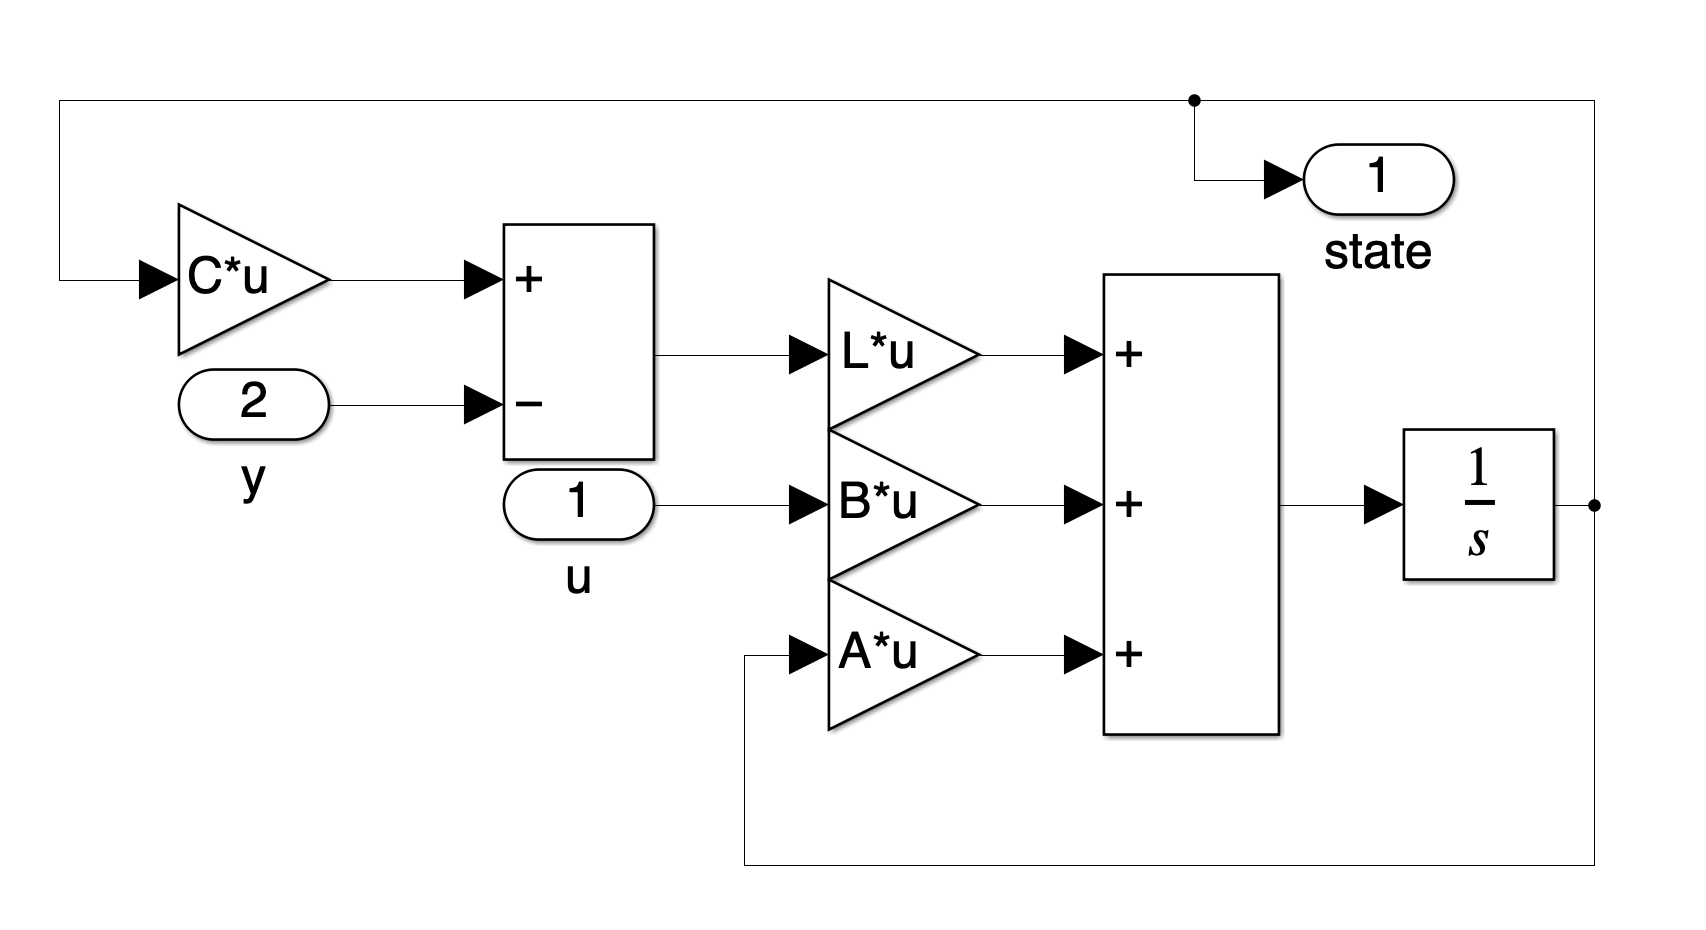
\includegraphics[width=0.7\textwidth]{media/observer_scheme.png}
    \caption{Схема наблюдателя}
    \label{fig:observer_scheme}
\end{figure}
\begin{figure}[ht!]
    \centering
    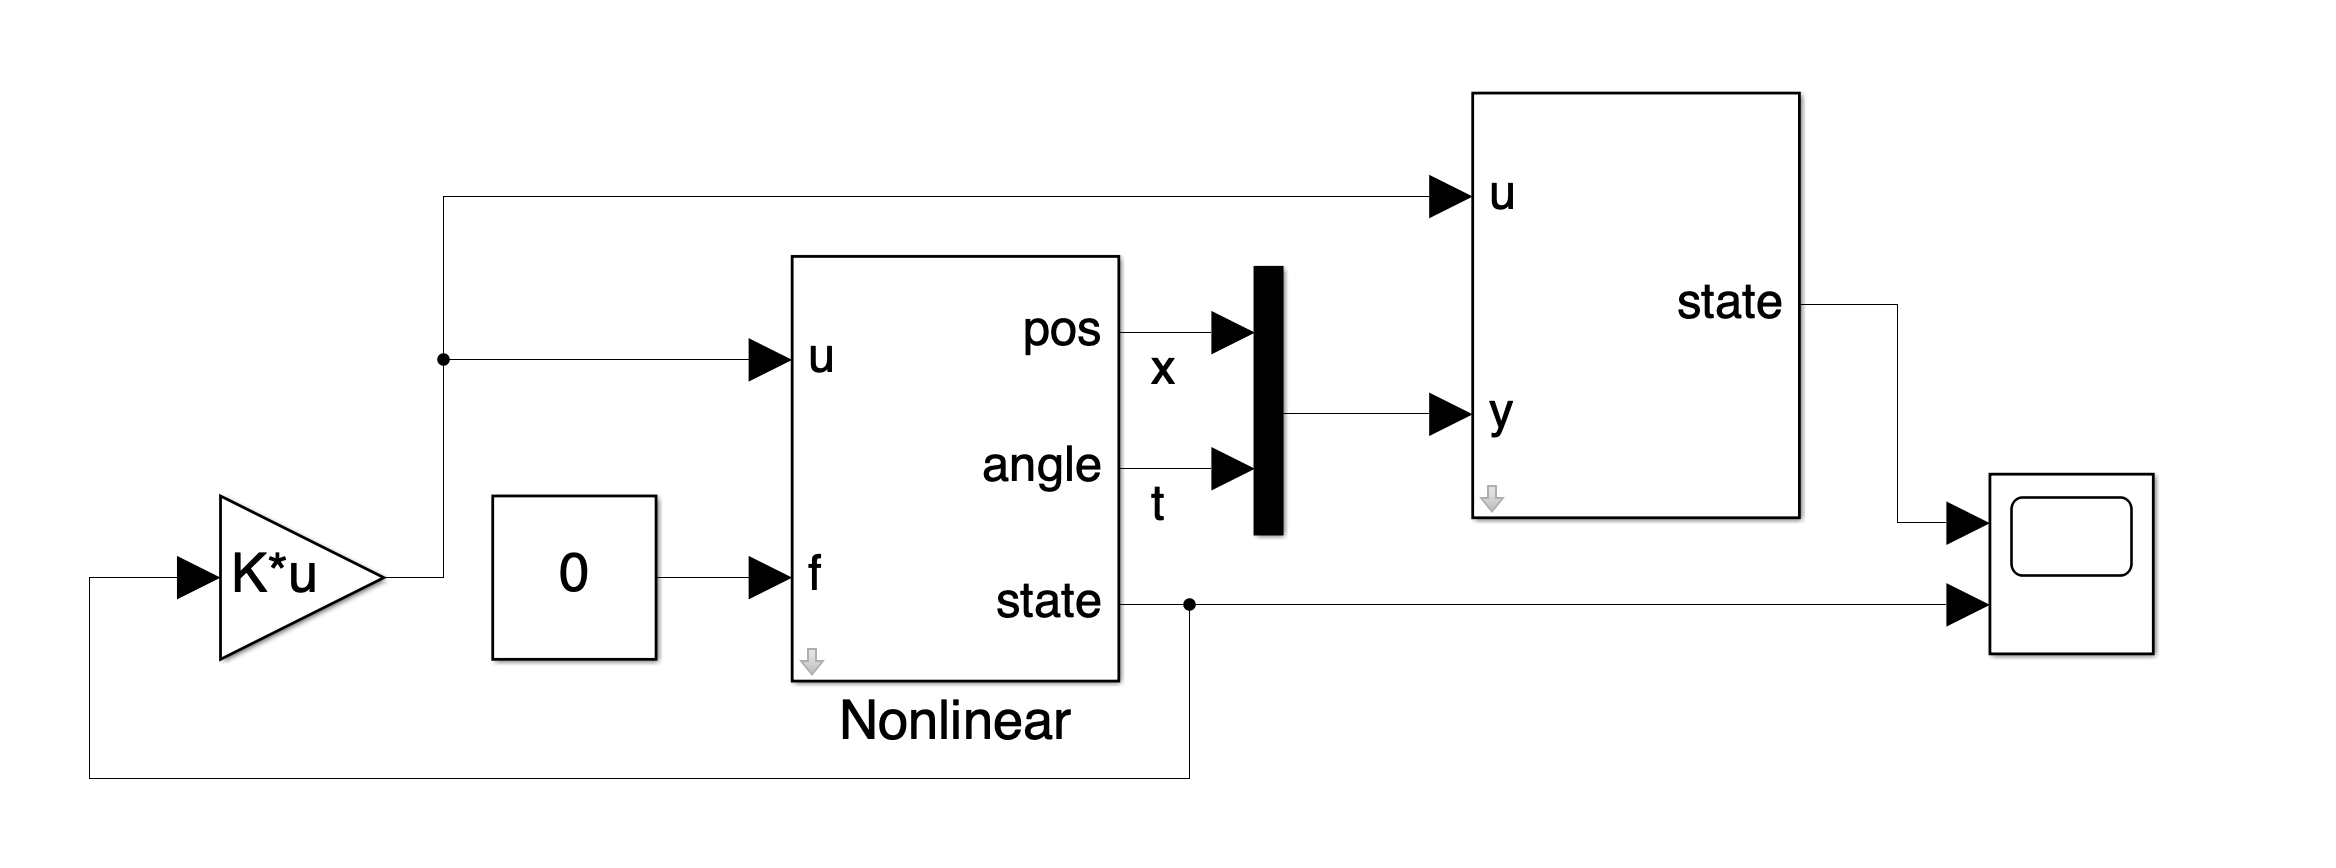
\includegraphics[width=0.7\textwidth]{media/observer_system.png}
    \caption{Схема включения наблюдателя в систему}
    \label{fig:observer_system}
\end{figure}

Результаты моделирования приведены на рисунке \ref{fig:observer_x_1} и рисунках \ref{fig:observer_x_cmp_1_sep}. 
\begin{figure}[ht!]
    \centering
    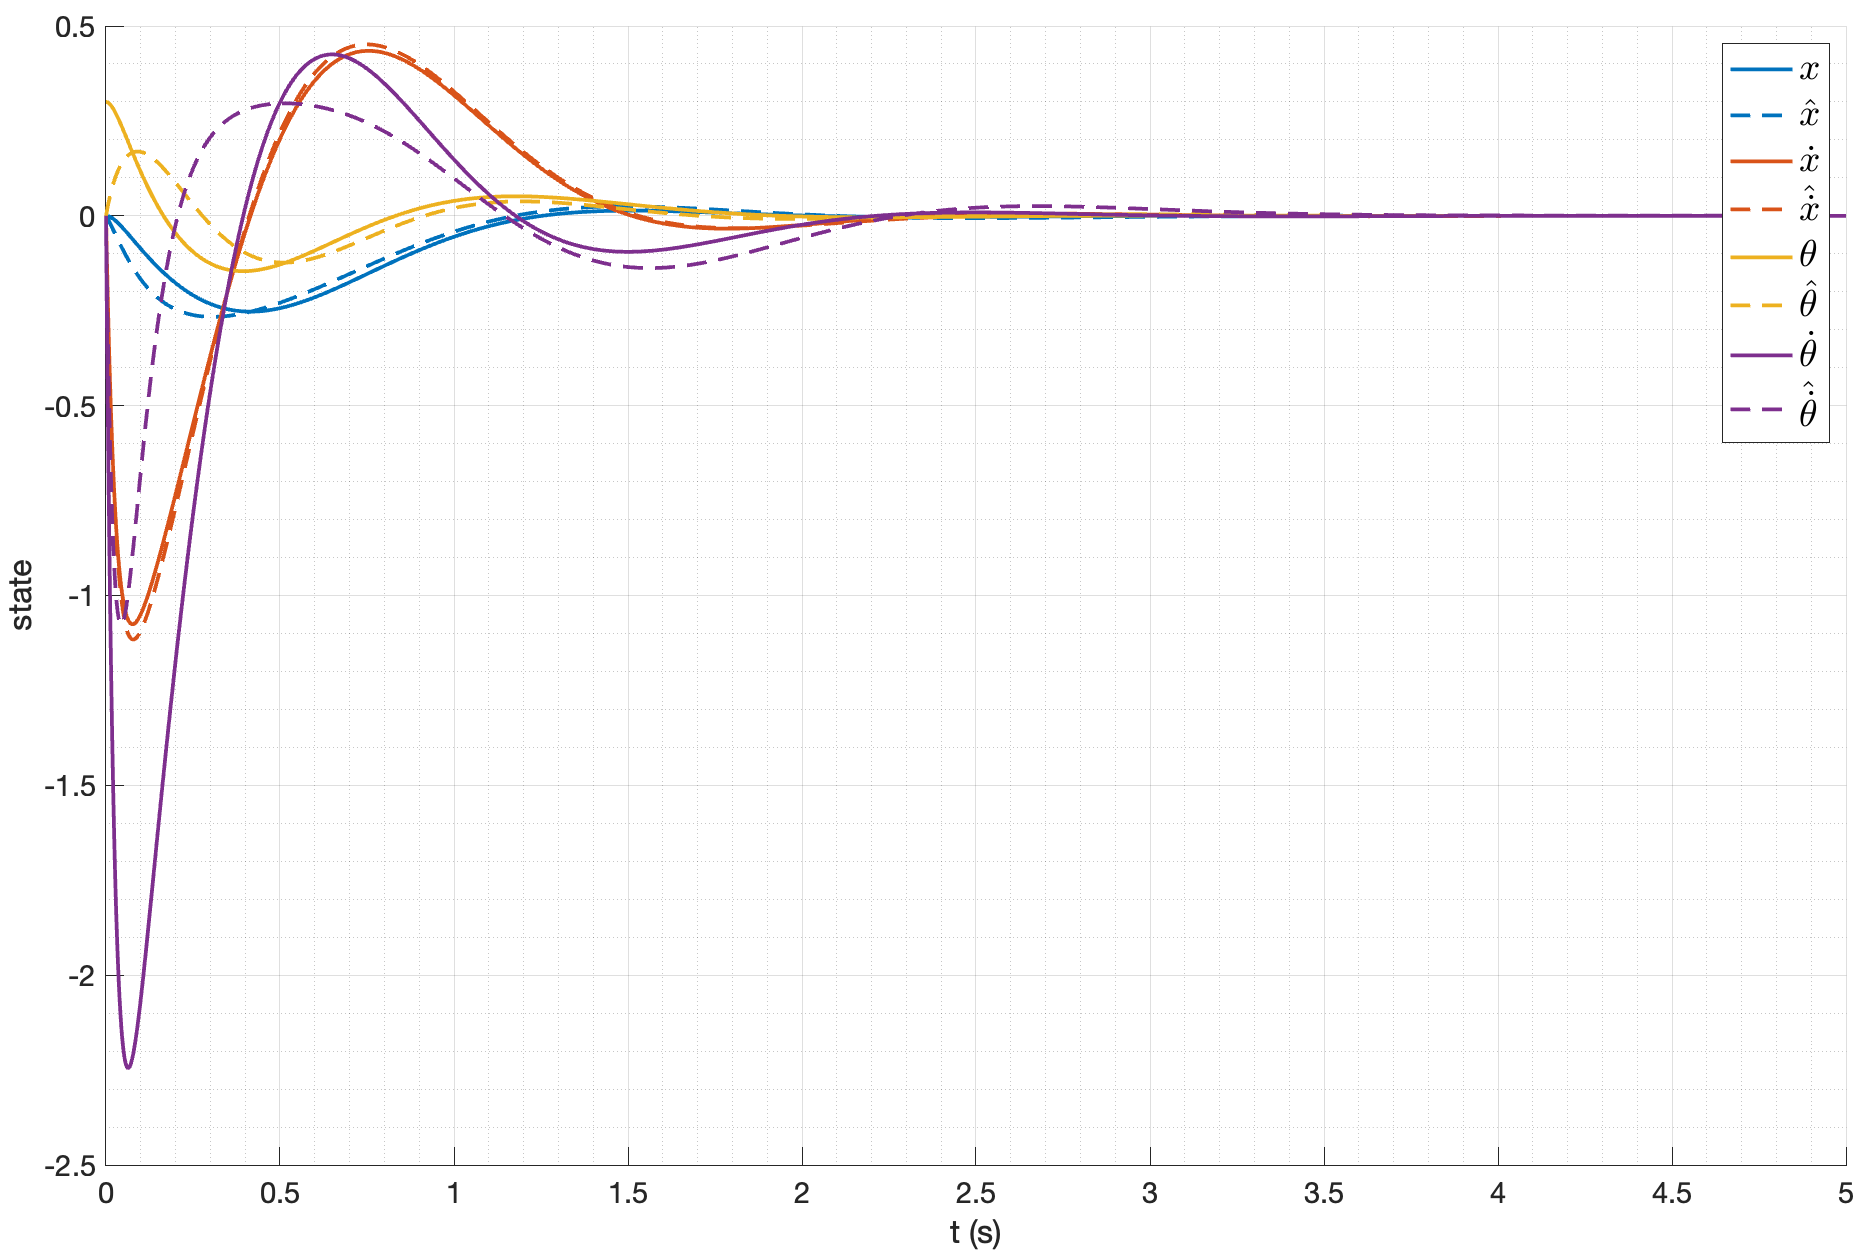
\includegraphics[width=\textwidth]{media/plots/modal_observer/observer_cmp_1.png}
    \caption{Результаты моделирования наблюдателя полного порядка}
    \label{fig:observer_x_1}
\end{figure}
\begin{figure}[ht!]
    \centering
    \begin{subfigure}[b]{0.45\textwidth}
        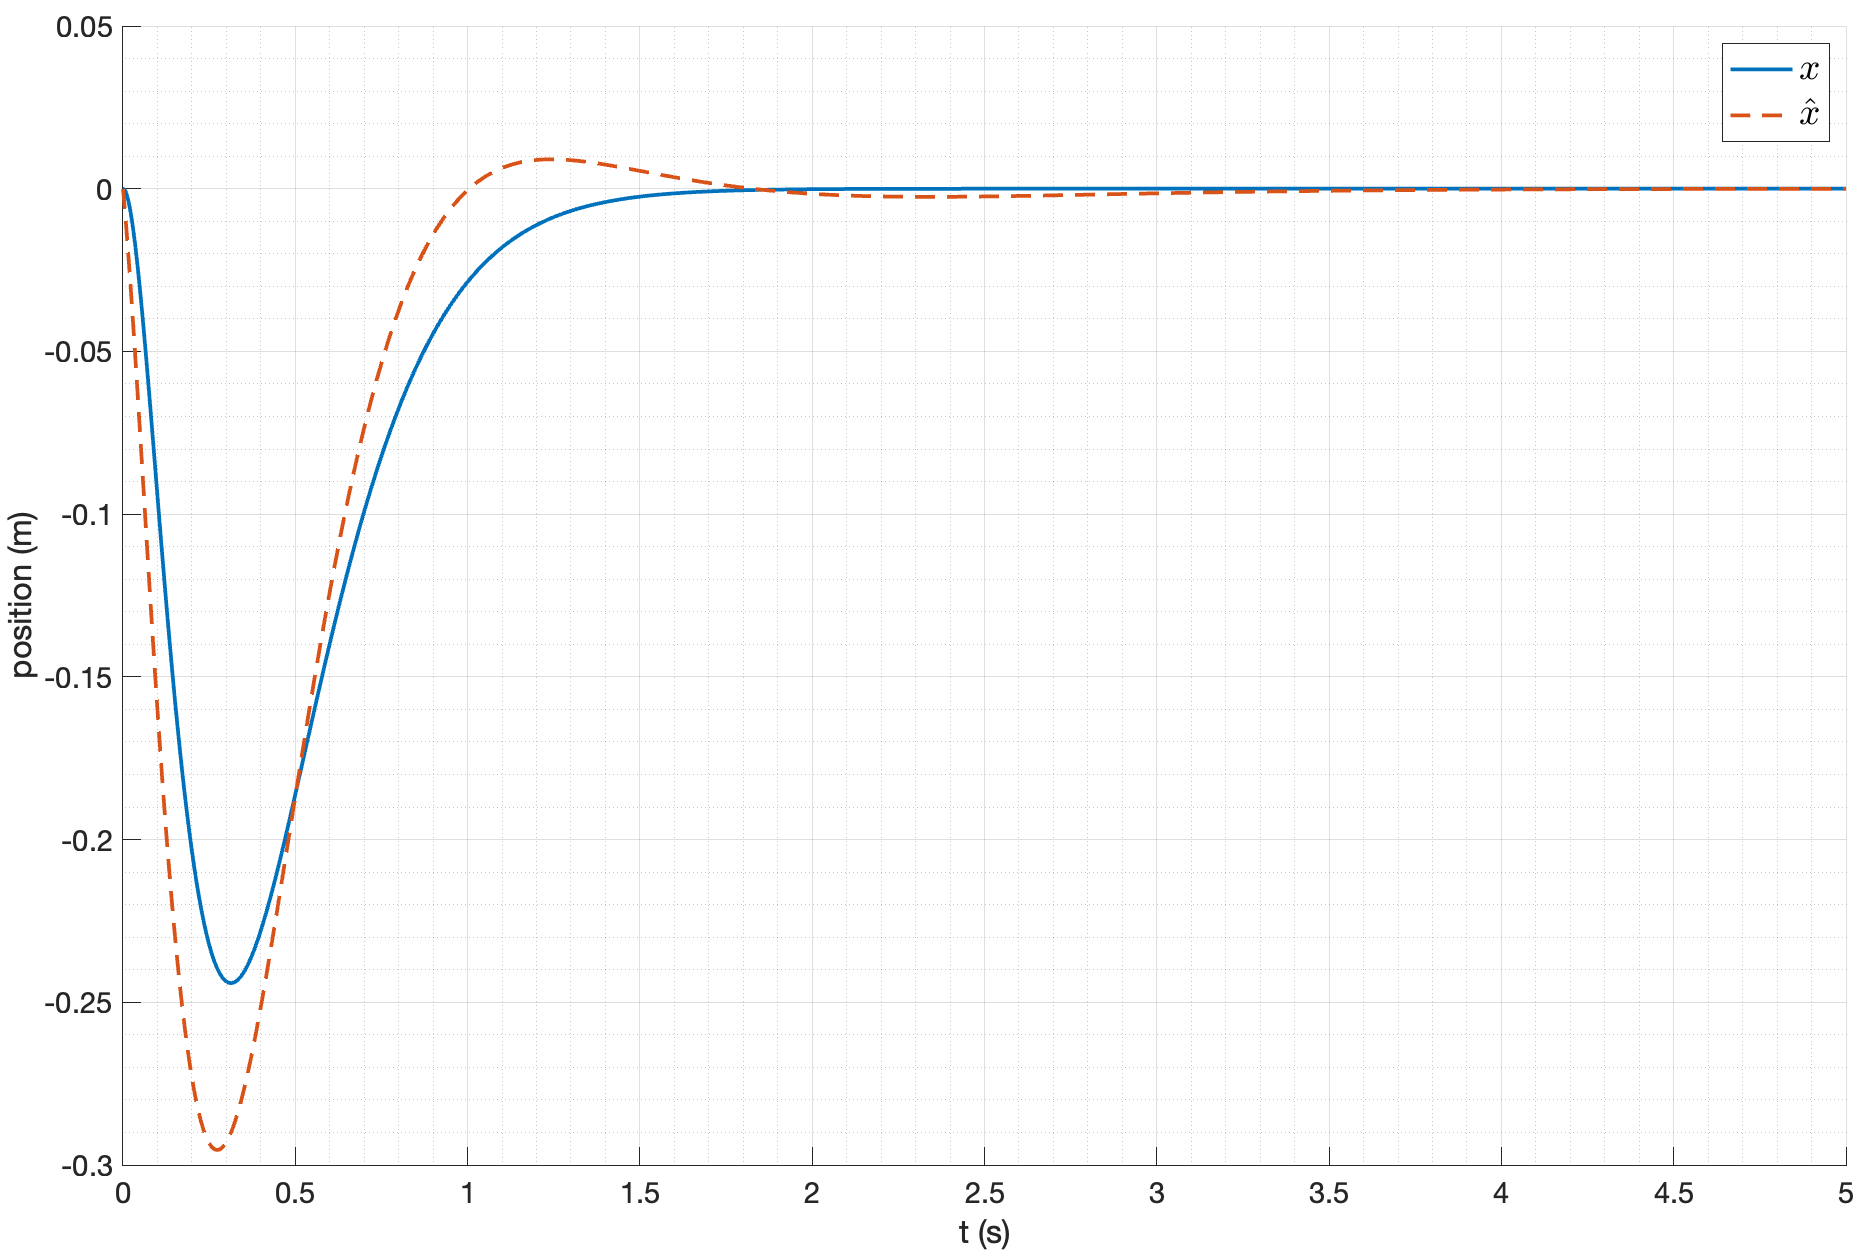
\includegraphics[width=\textwidth]{media/plots/modal_observer/observer_x_cmp_1.png}
        \caption{Оценка координаты тележки}
        \label{fig:observer_x_cmp_1}
    \end{subfigure}
    \begin{subfigure}[b]{0.45\textwidth}
        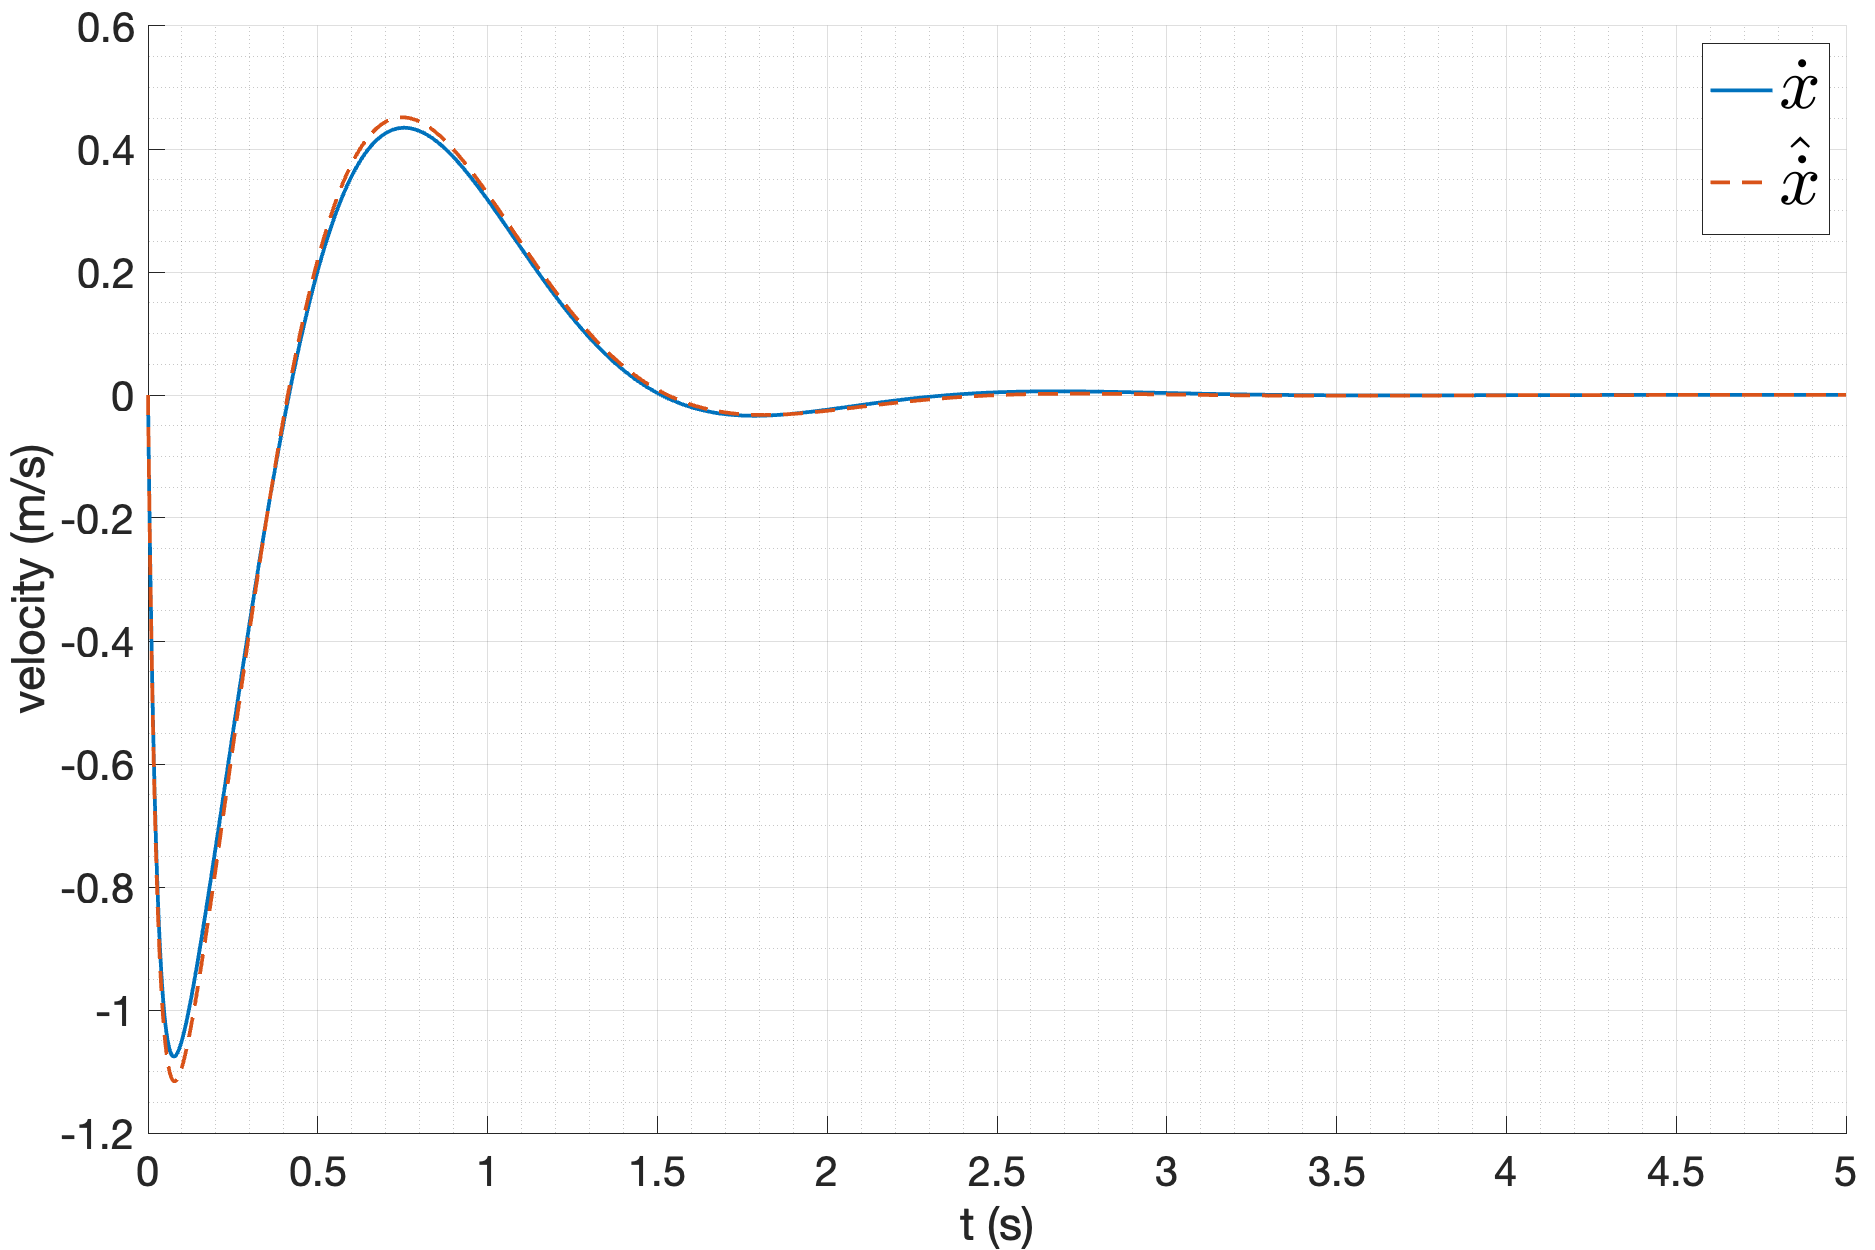
\includegraphics[width=\textwidth]{media/plots/modal_observer/observer_dotx_cmp_1.png}
        \caption{Оценка скорости тележки}
        \label{fig:observer_dotx_cmp_1}
    \end{subfigure}
    \begin{subfigure}[b]{0.45\textwidth}
        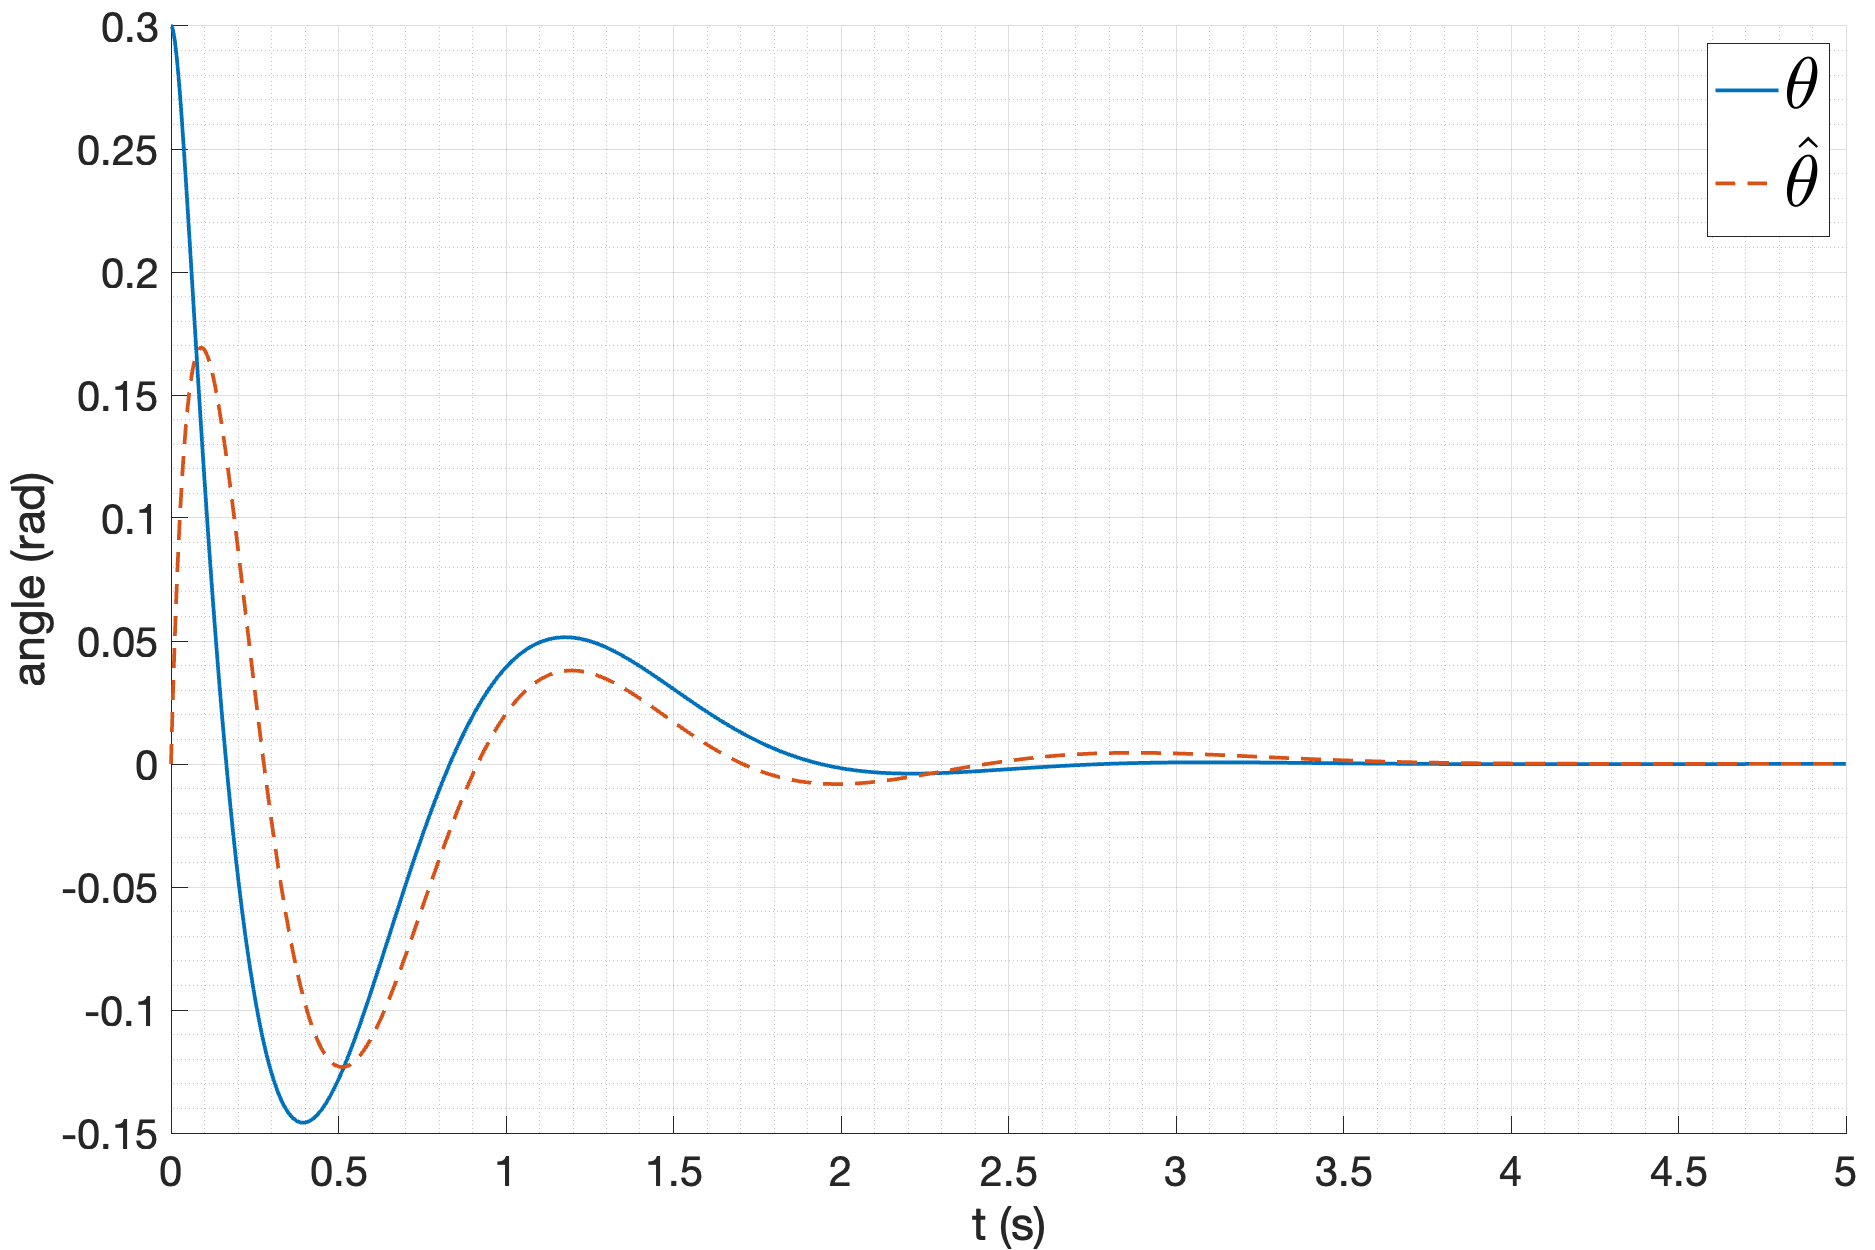
\includegraphics[width=\textwidth]{media/plots/modal_observer/observer_theta_cmp_1.png}
        \caption{Оценка угла отклонения маятника}
        \label{fig:observer_theta_cmp_1}
    \end{subfigure}
    \begin{subfigure}[b]{0.45\textwidth}
        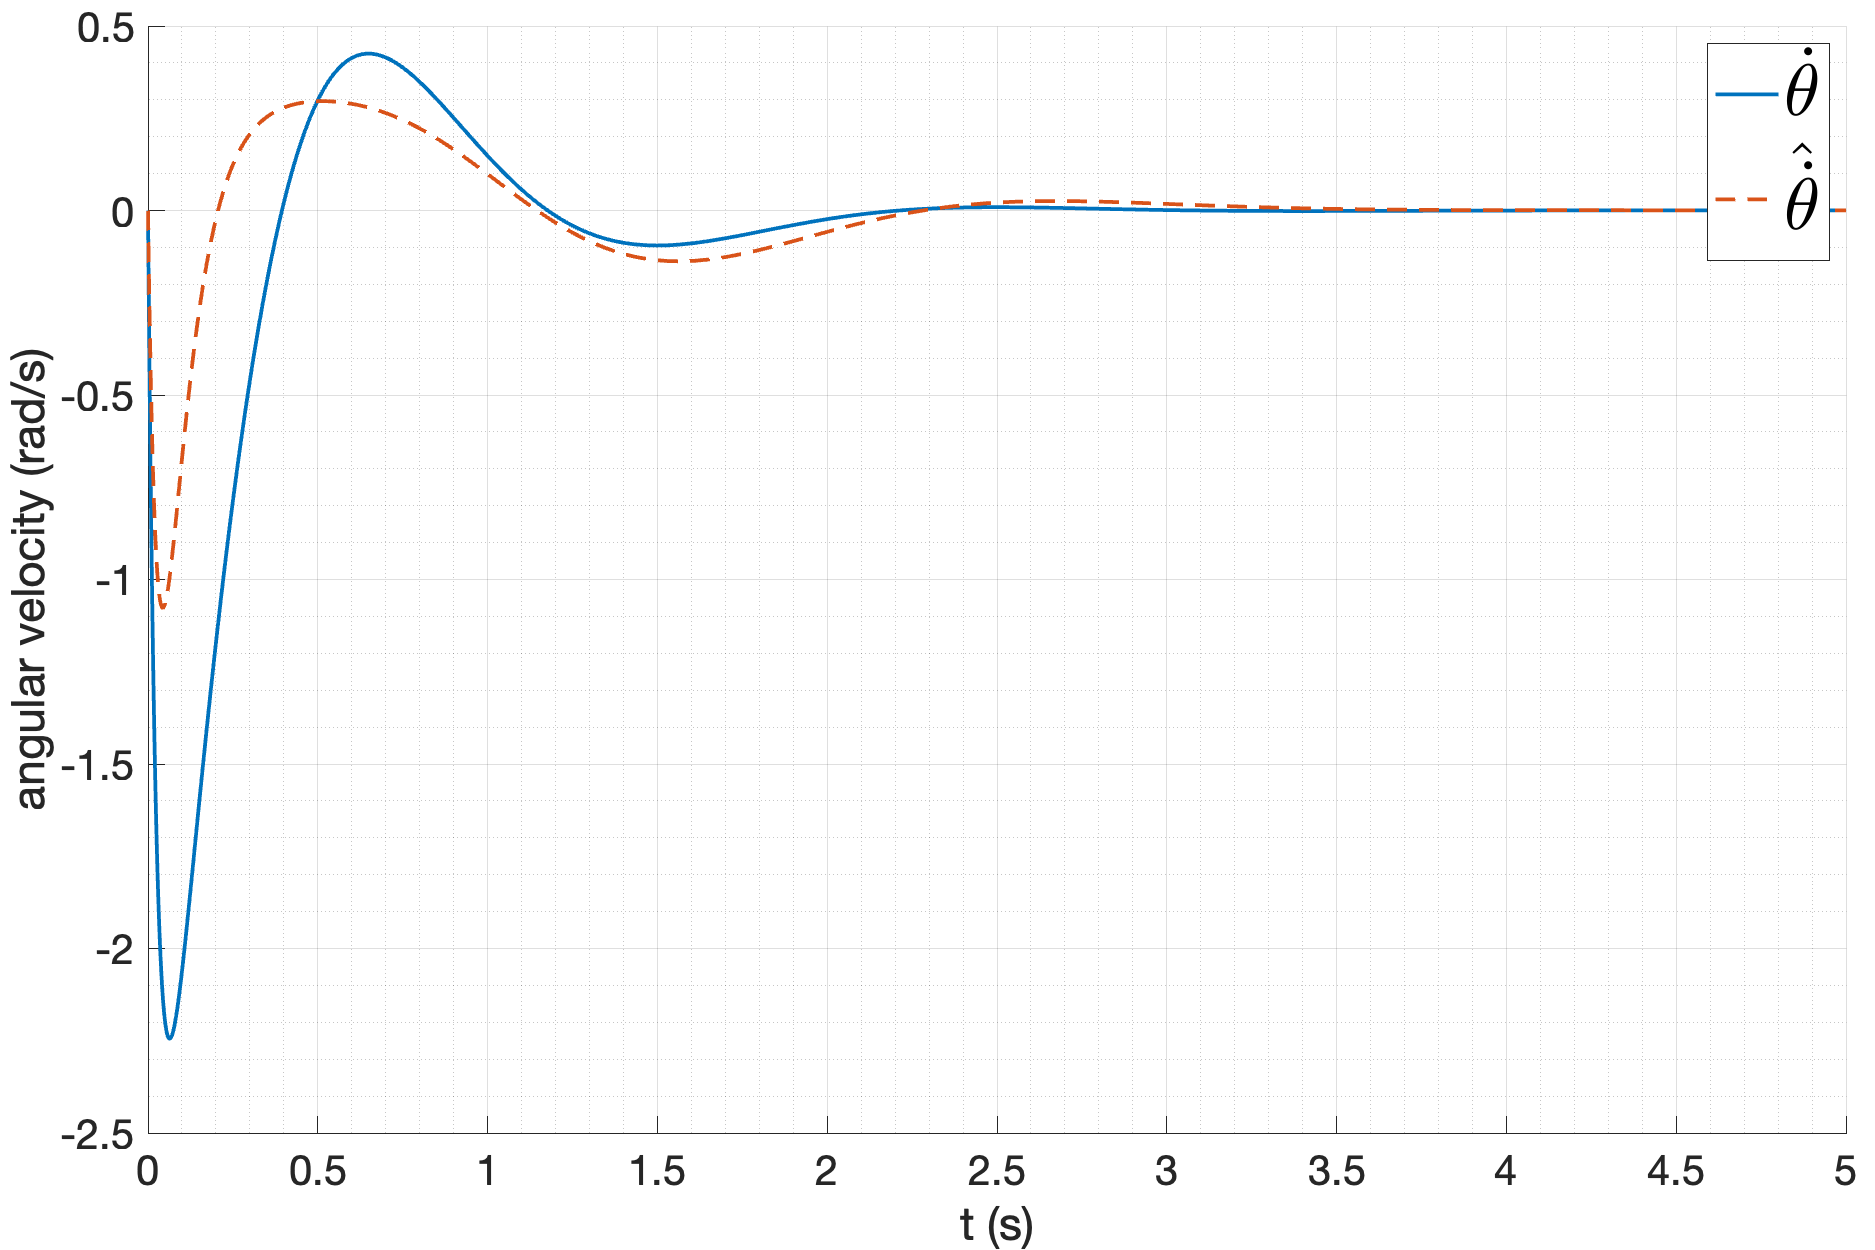
\includegraphics[width=\textwidth]{media/plots/modal_observer/observer_dottheta_cmp_1.png}
        \caption{Оценка угловой скорости маятника}
        \label{fig:observer_dottheta_cmp_1}
    \end{subfigure}
    \caption{Сравнение оценок состояния системы с реальным состоянием}
    \label{fig:observer_x_cmp_1_sep}
\end{figure}
\FloatBarrier
Можно увидеть, что оценка состояния нелинейной системы наблюдателем полного порядка
сходится к реальному состоянию системы, при этом время переходного процесса составляет около 2 секунд.
График ошибки оценки состояния системы приведен на рисунке \ref{fig:observer_err_1}.
\begin{figure}[ht!]
    \centering
    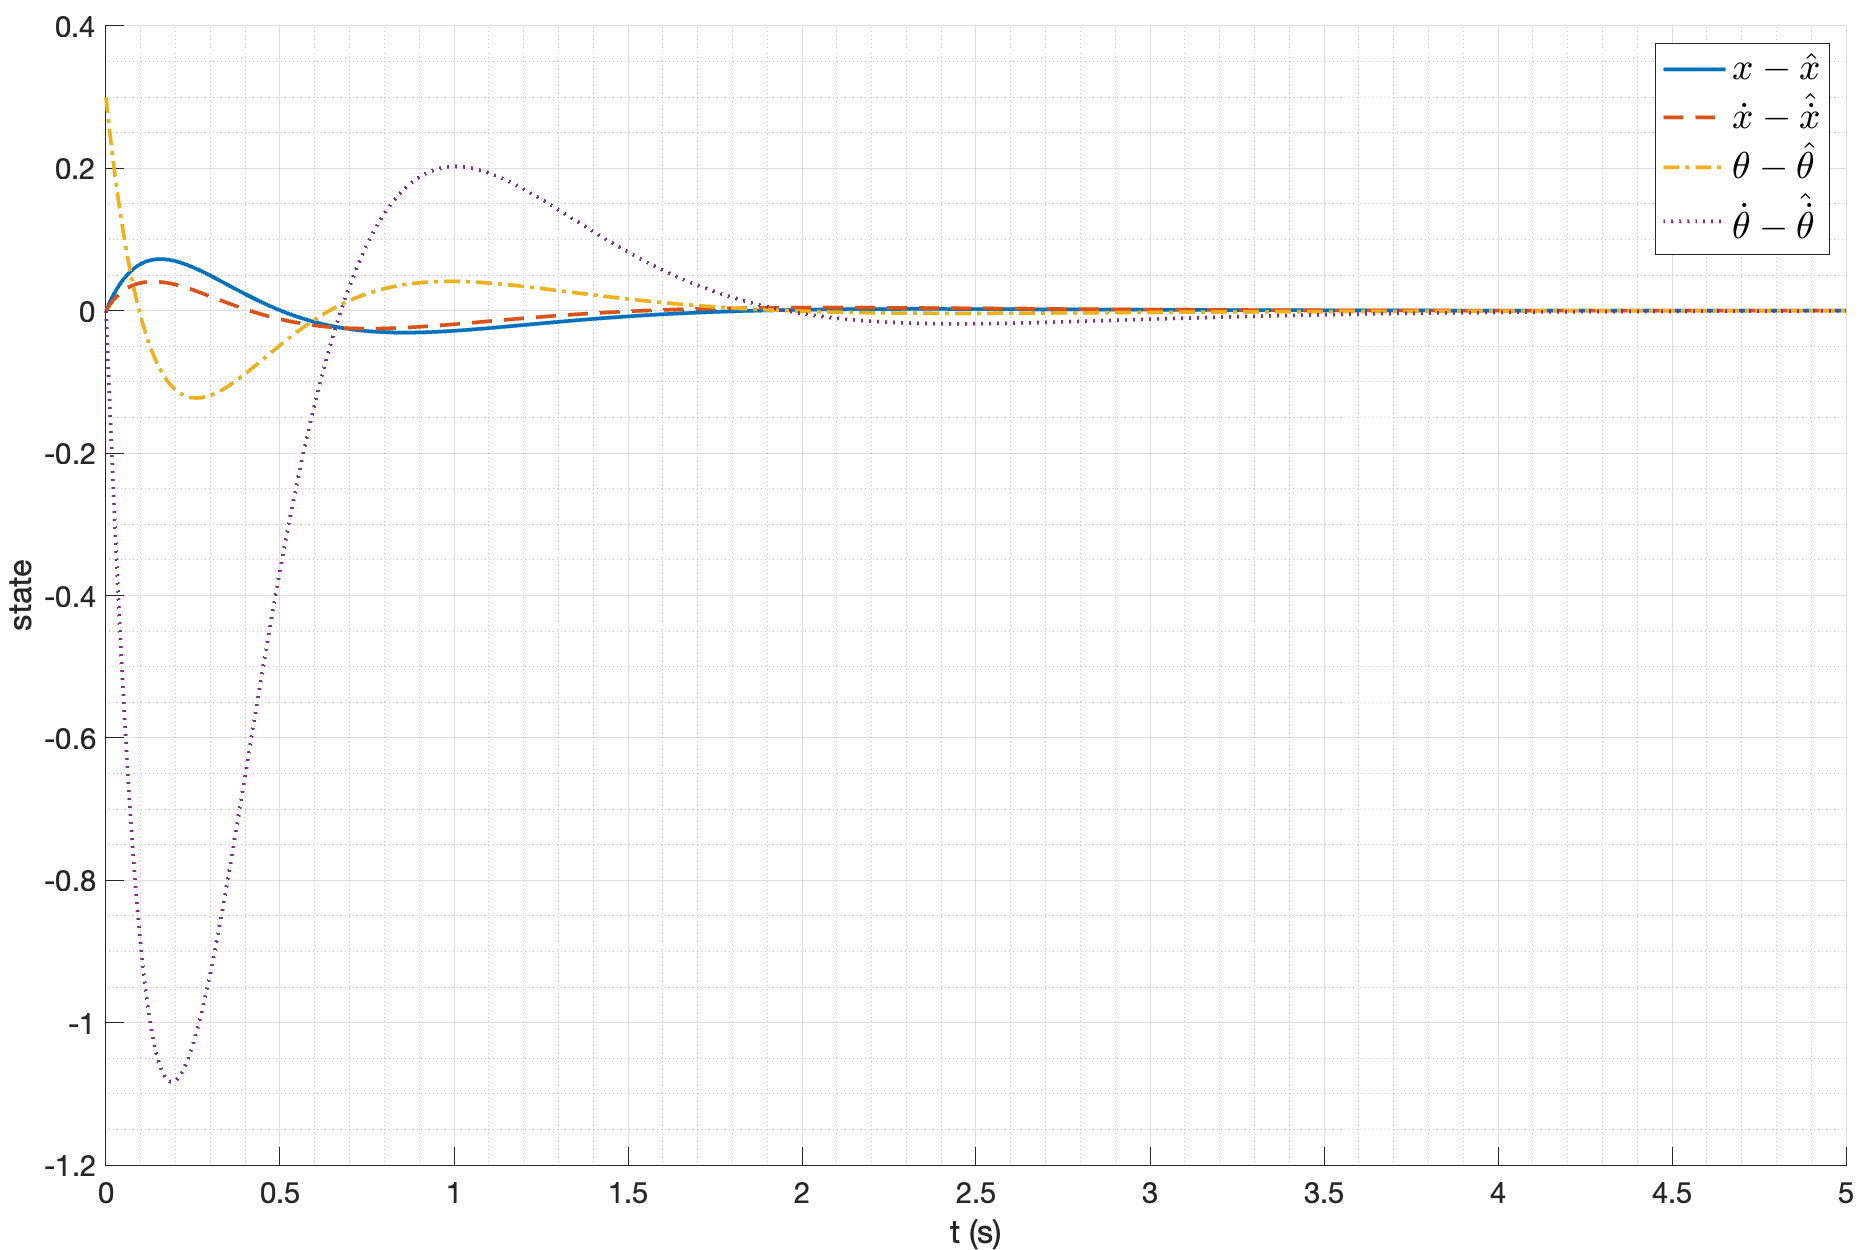
\includegraphics[width=\textwidth]{media/plots/modal_observer/observer_err_1.png}
    \caption{Ошибка оценки состояния системы наблюдателем полного порядка}
    \label{fig:observer_err_1}
\end{figure} 

Теперь посмотрим на работу наблюдателя полного порядка с более большим по модулю спектром, например, 
$\begin{bmatrix}-10 & -10 & -10 & -10\end{bmatrix}$. Результаты моделирования приведены на
рисунке \ref{fig:observer_x_2} и \ref{fig:observer_x_cmp_2_sep}. 
\begin{figure}[ht!]
    \centering
    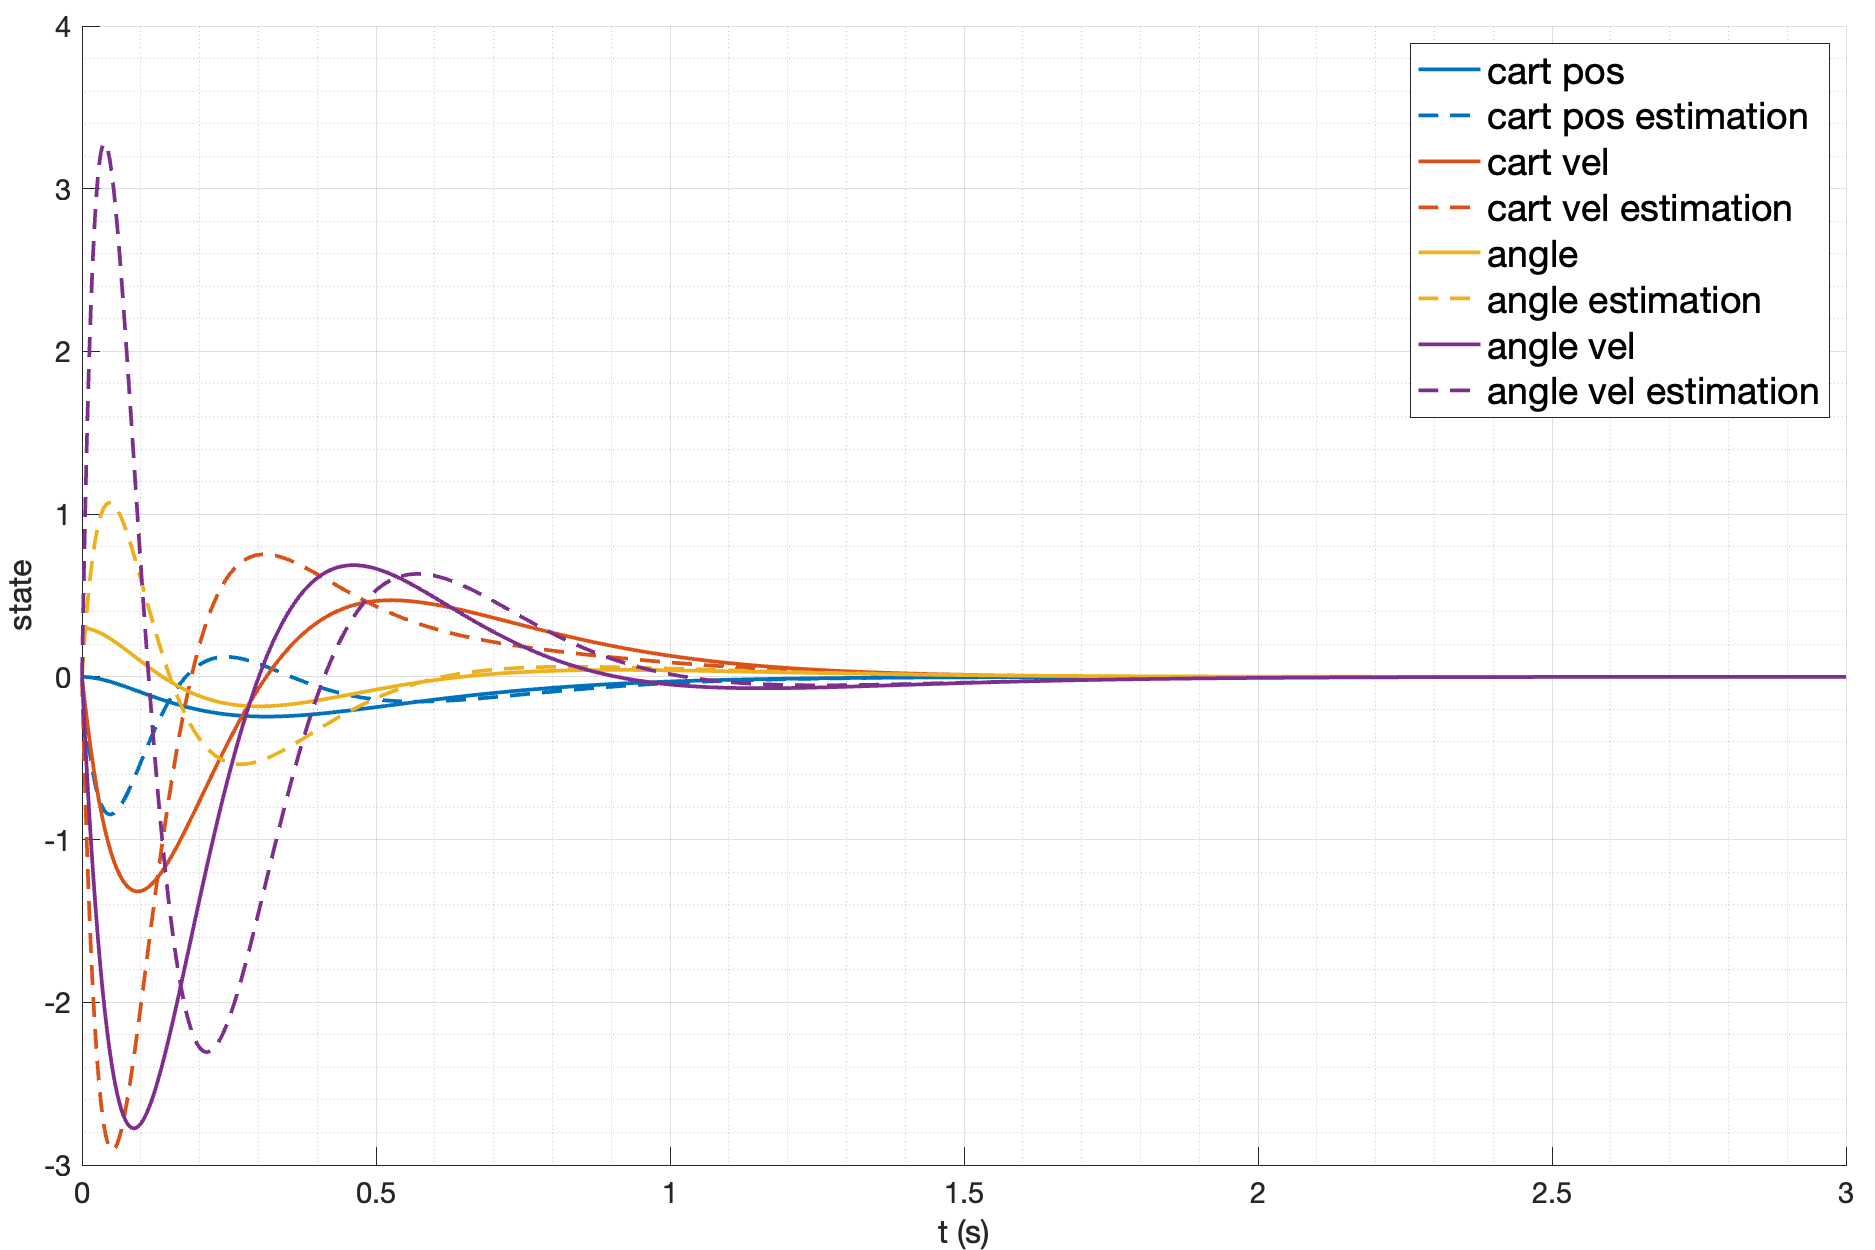
\includegraphics[width=\textwidth]{media/plots/modal_observer/observer_cmp_2.png}
    \caption{Результаты моделирования наблюдателя полного порядка}
    \label{fig:observer_x_2}
\end{figure}

\begin{figure}[ht!]
    \centering
    \begin{subfigure}[b]{0.45\textwidth}
        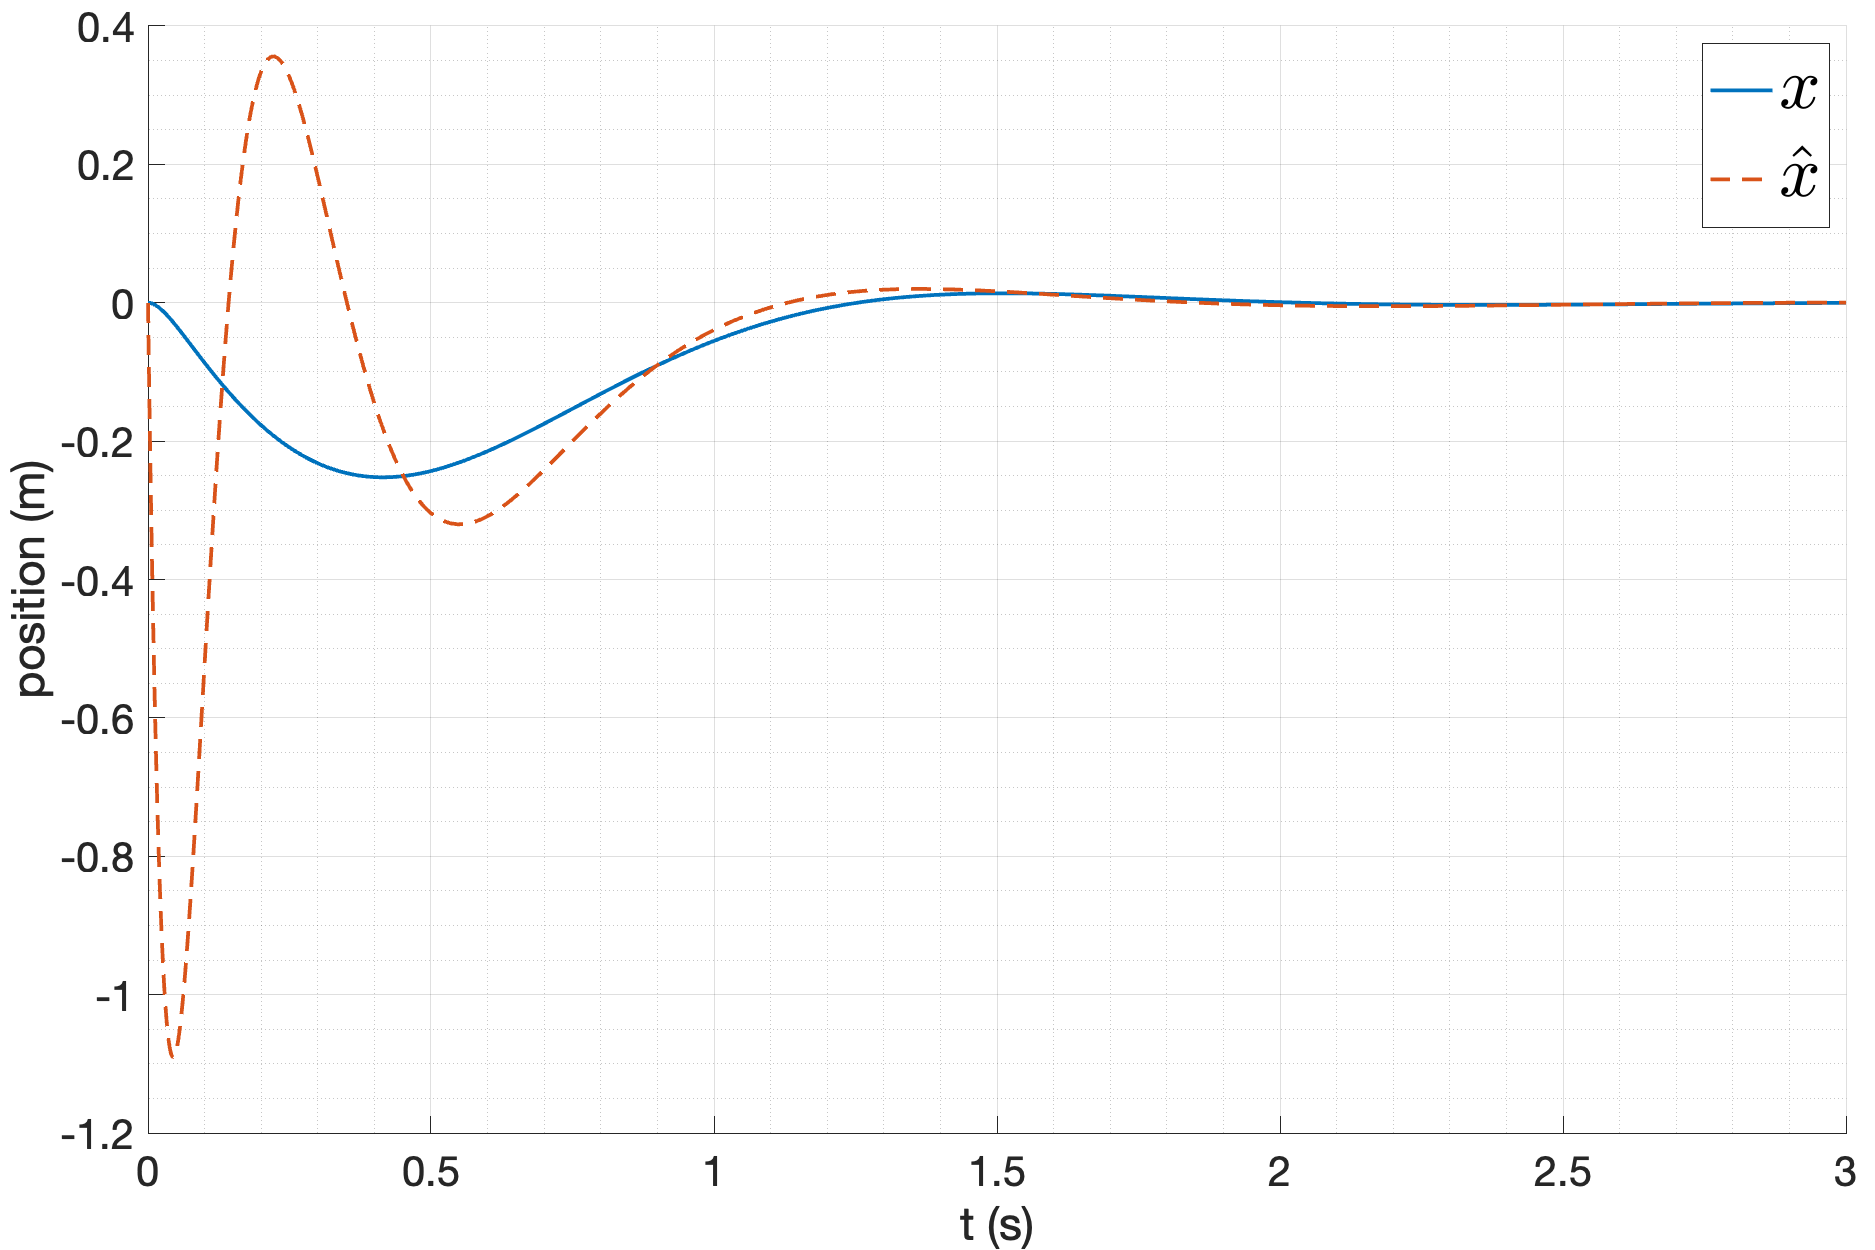
\includegraphics[width=\textwidth]{media/plots/modal_observer/observer_x_cmp_2.png}
        \caption{Оценка координаты тележки}
        \label{fig:observer_x_cmp_2}
    \end{subfigure}
    \begin{subfigure}[b]{0.45\textwidth}
        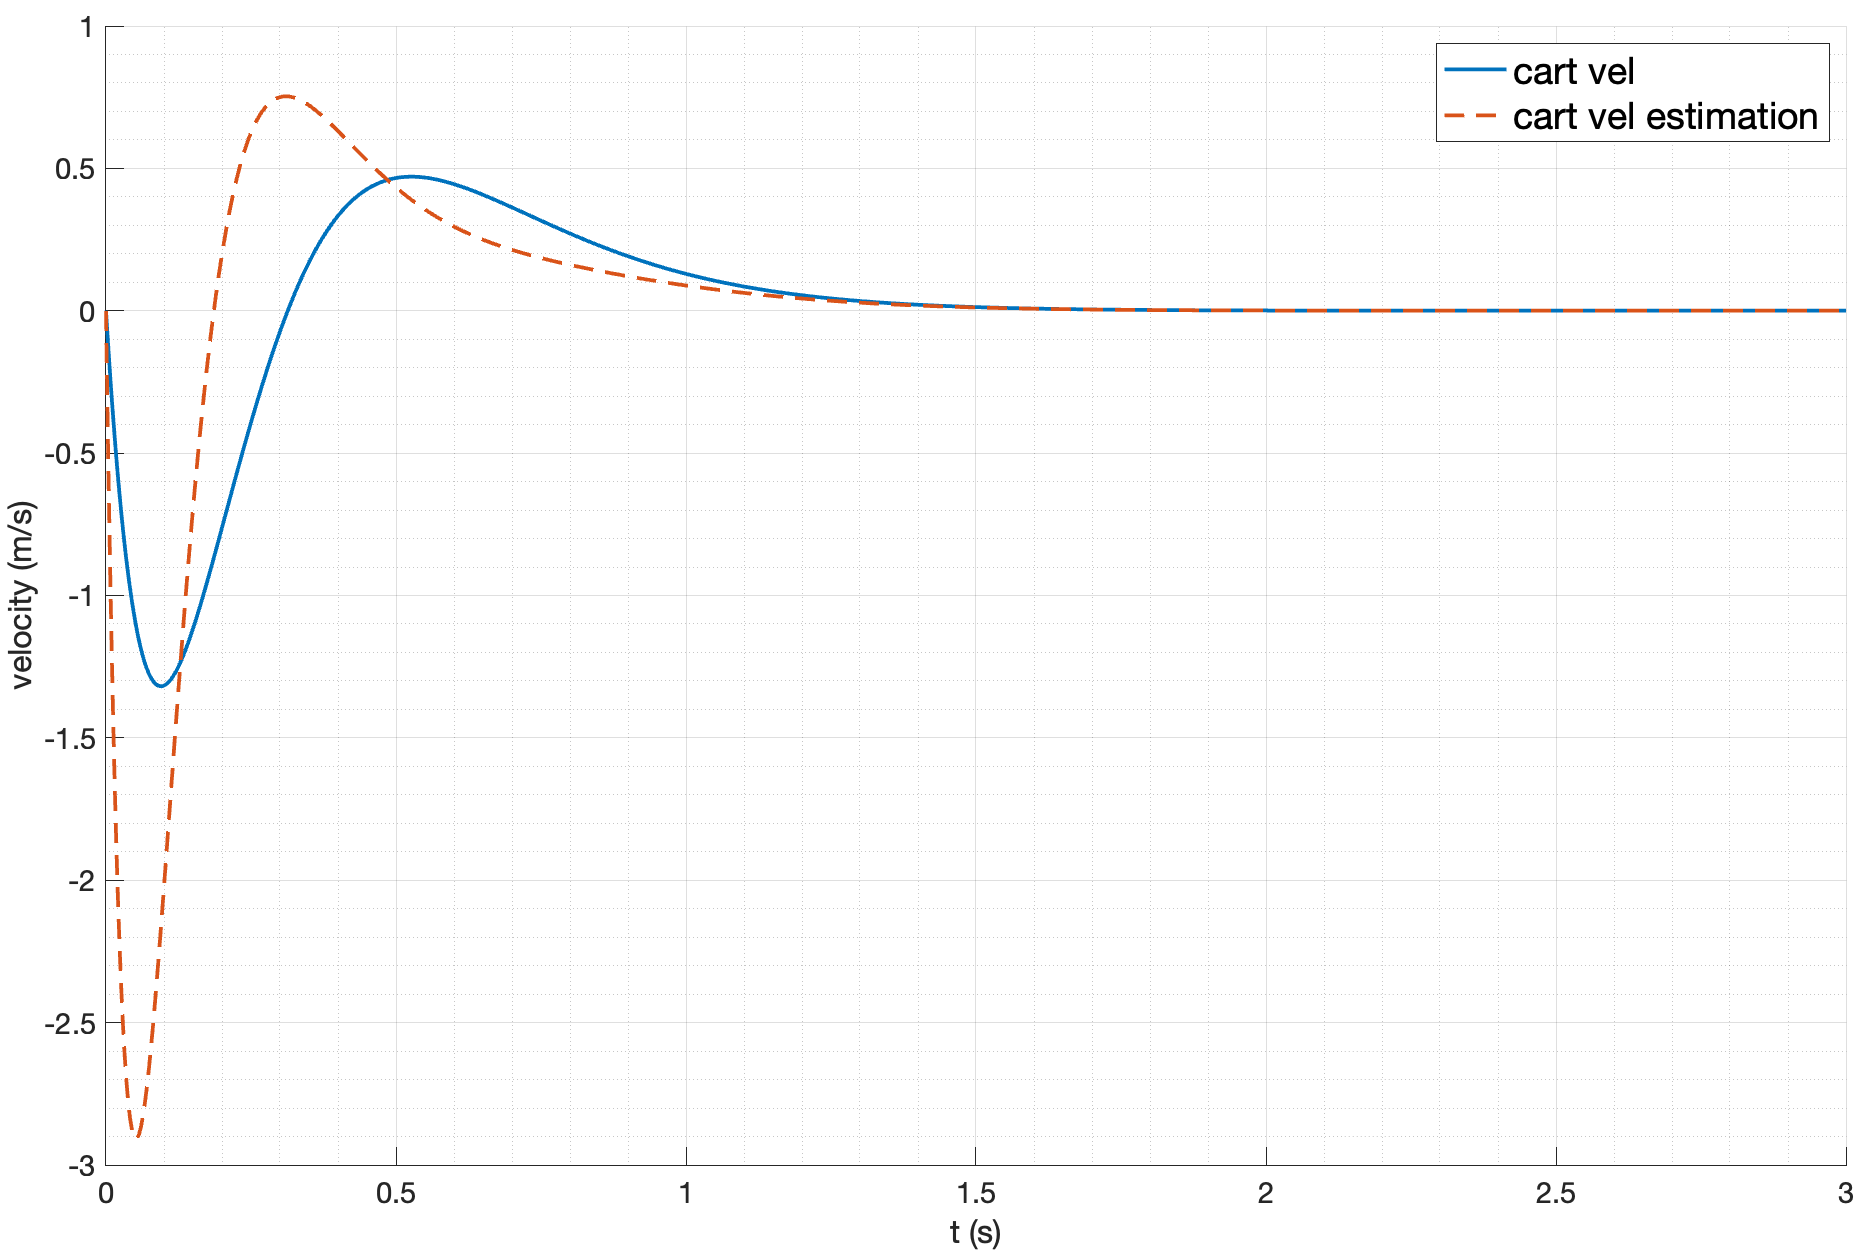
\includegraphics[width=\textwidth]{media/plots/modal_observer/observer_dotx_cmp_2.png}
        \caption{Оценка скорости тележки}
        \label{fig:observer_dotx_cmp_2}
    \end{subfigure}
    \begin{subfigure}[b]{0.45\textwidth}
        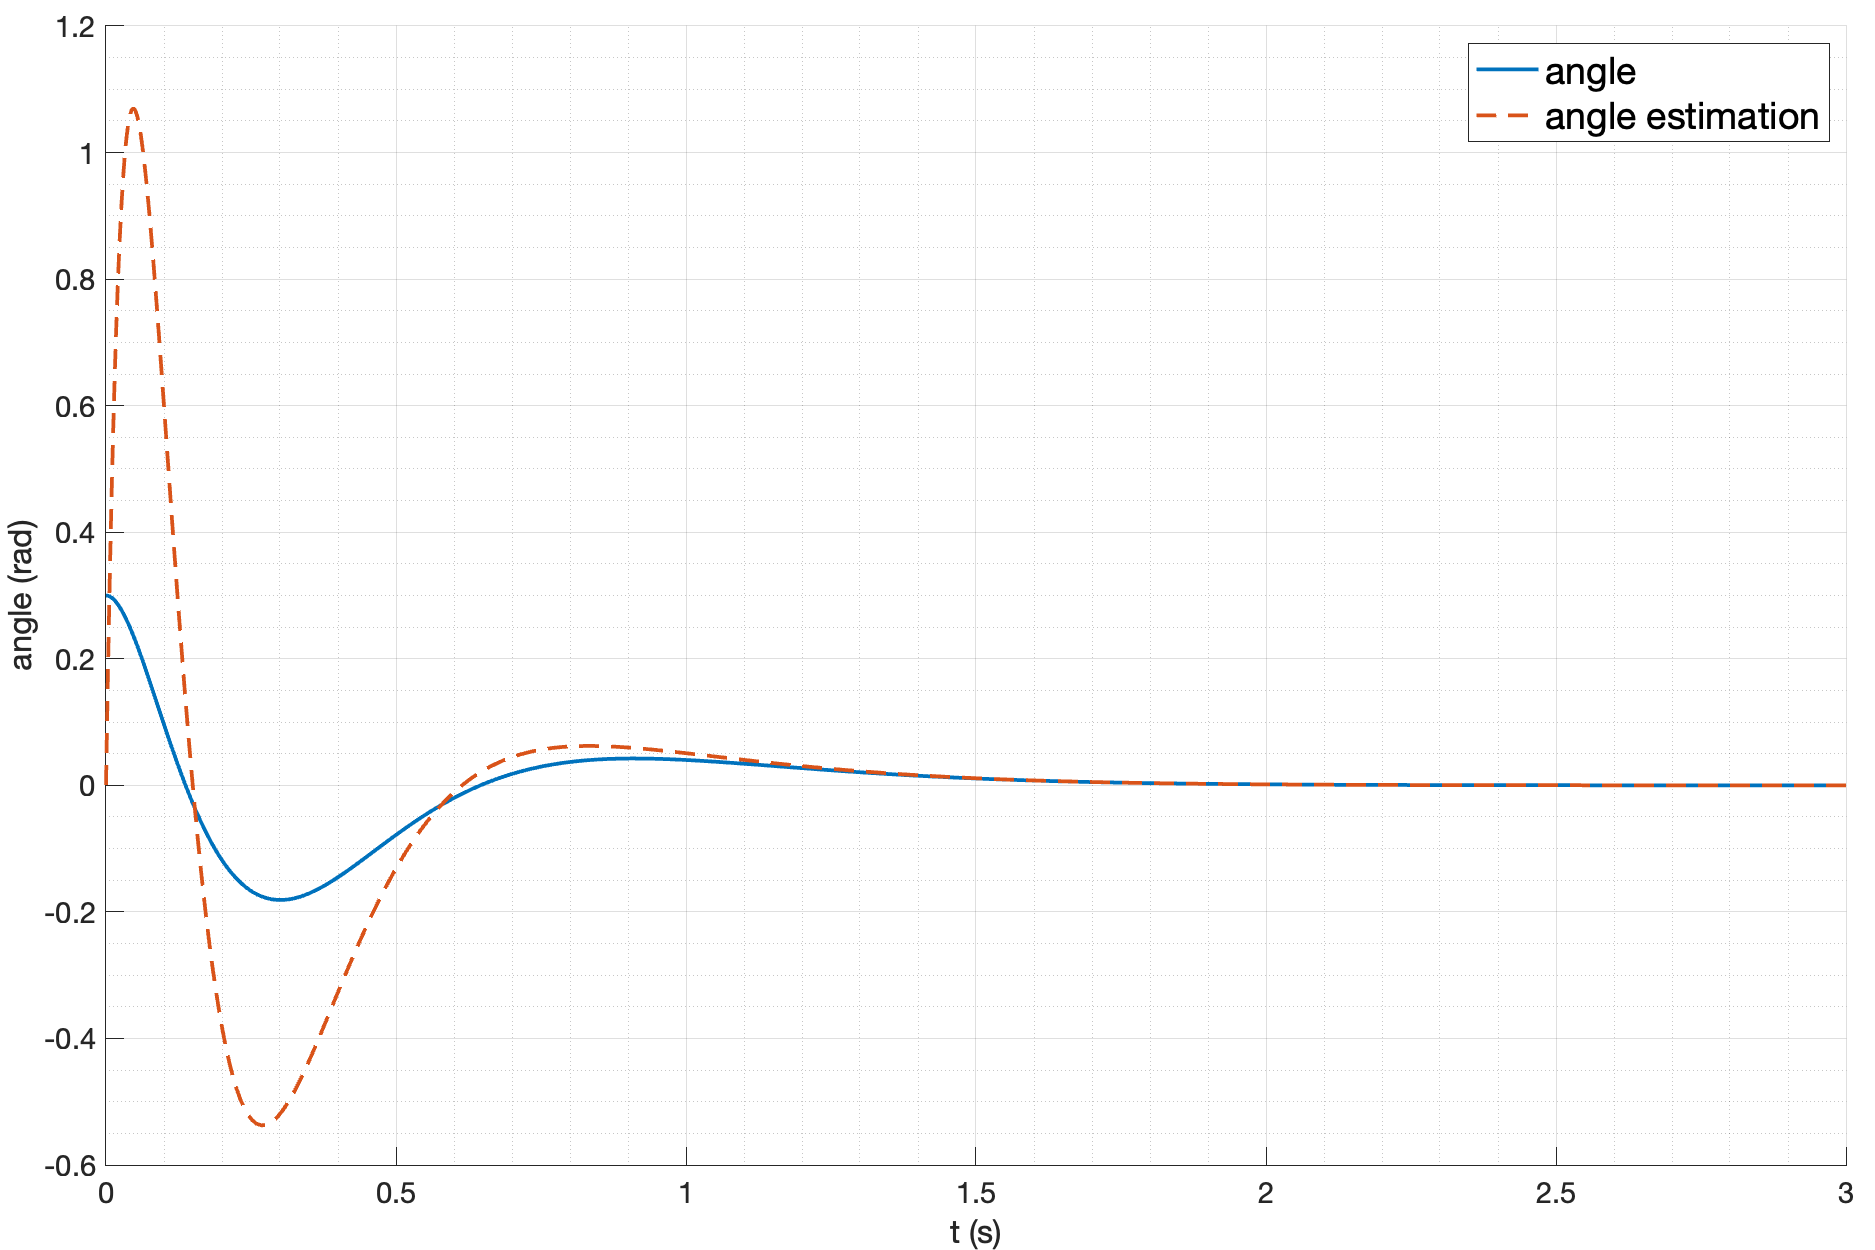
\includegraphics[width=\textwidth]{media/plots/modal_observer/observer_theta_cmp_2.png}
        \caption{Оценка угла отклонения маятника}
        \label{fig:observer_theta_cmp_2}
    \end{subfigure}
    \begin{subfigure}[b]{0.45\textwidth}
        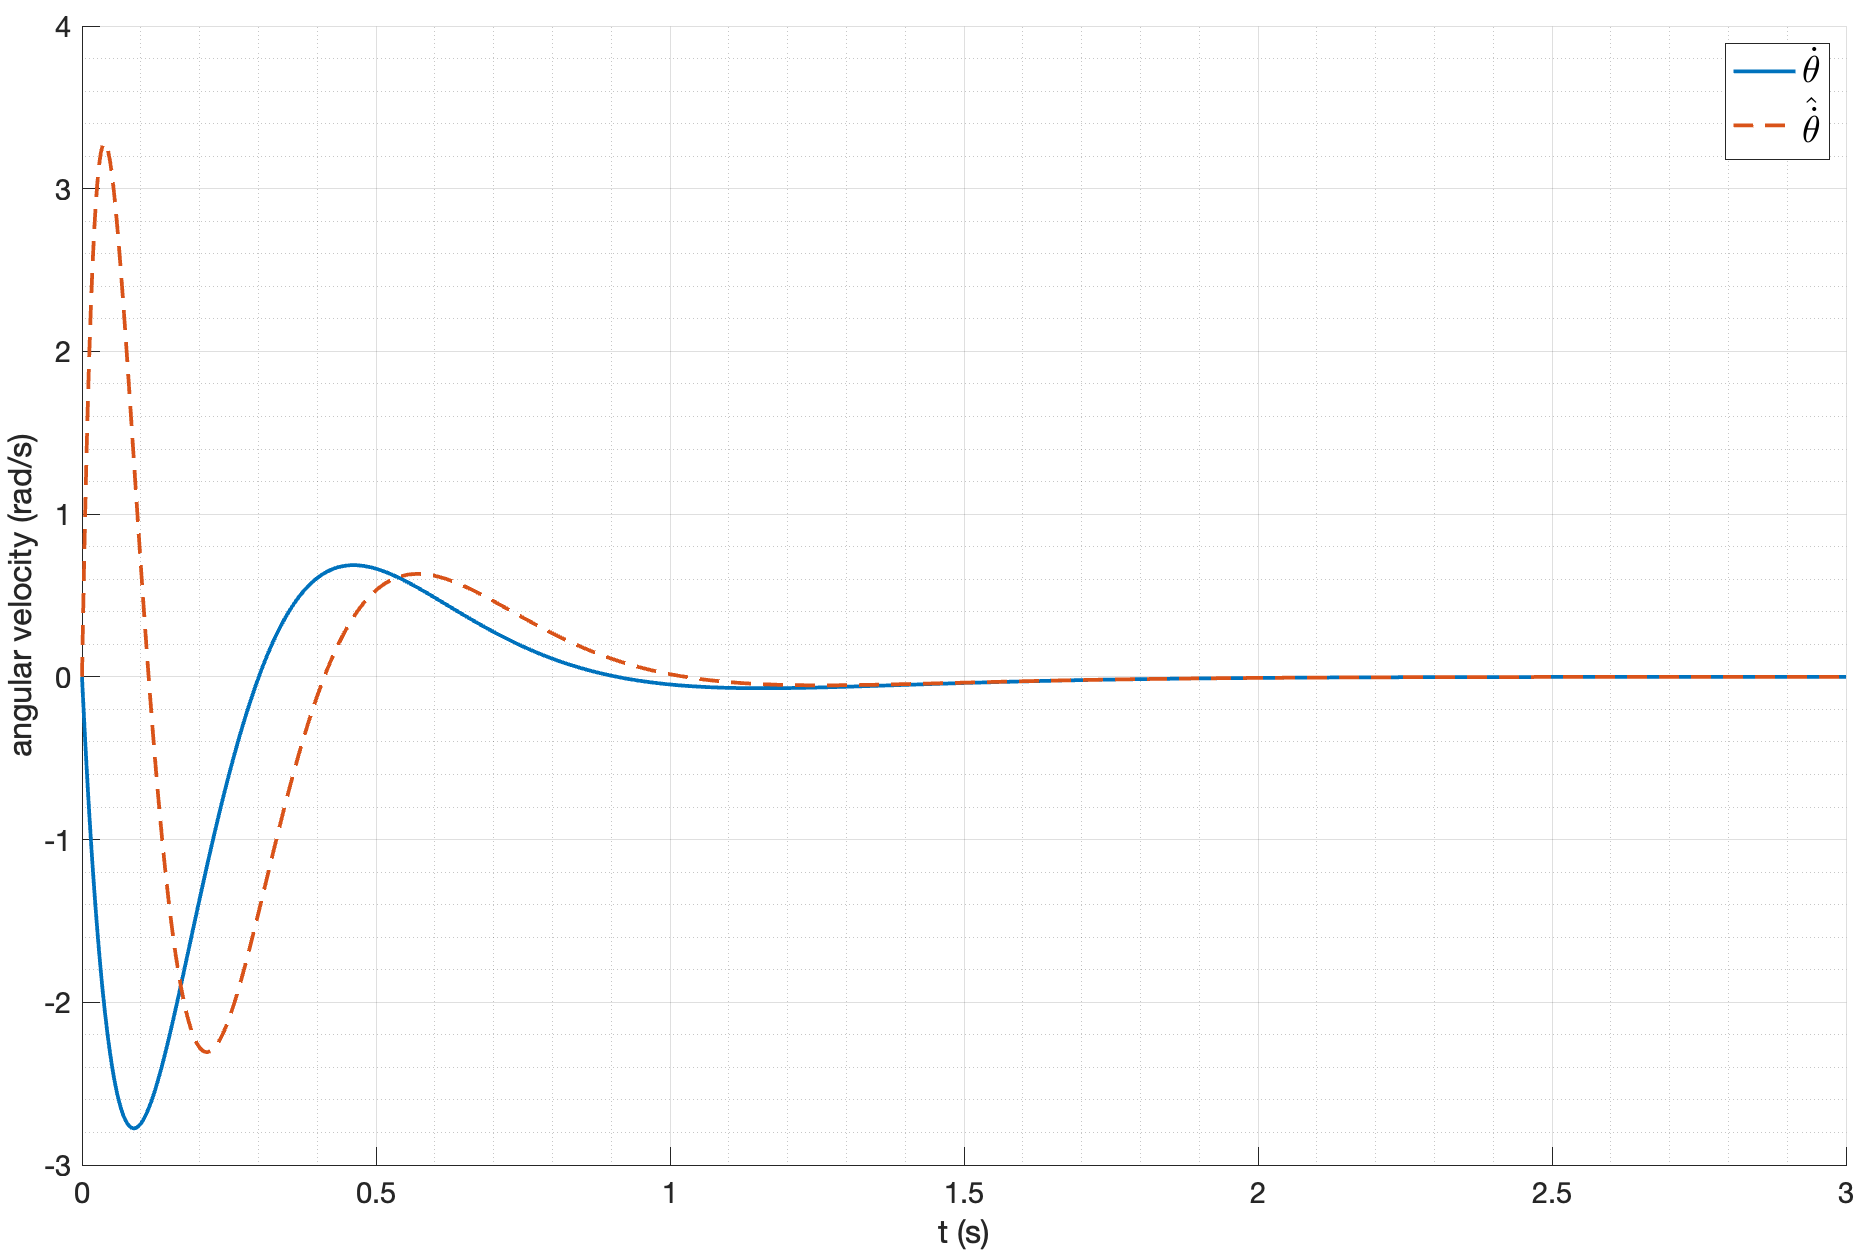
\includegraphics[width=\textwidth]{media/plots/modal_observer/observer_dottheta_cmp_2.png}
        \caption{Оценка угловой скорости маятника}
        \label{fig:observer_dottheta_cmp_2}
    \end{subfigure}
    \caption{Сравнение оценок состояния системы с реальным состоянием при $k = -10$}
    \label{fig:observer_x_cmp_2_sep}
\end{figure}
График ошибки оценки состояния системы приведен на рисунке \ref{fig:observer_err_2}.
\begin{figure}[ht!]
    \centering
    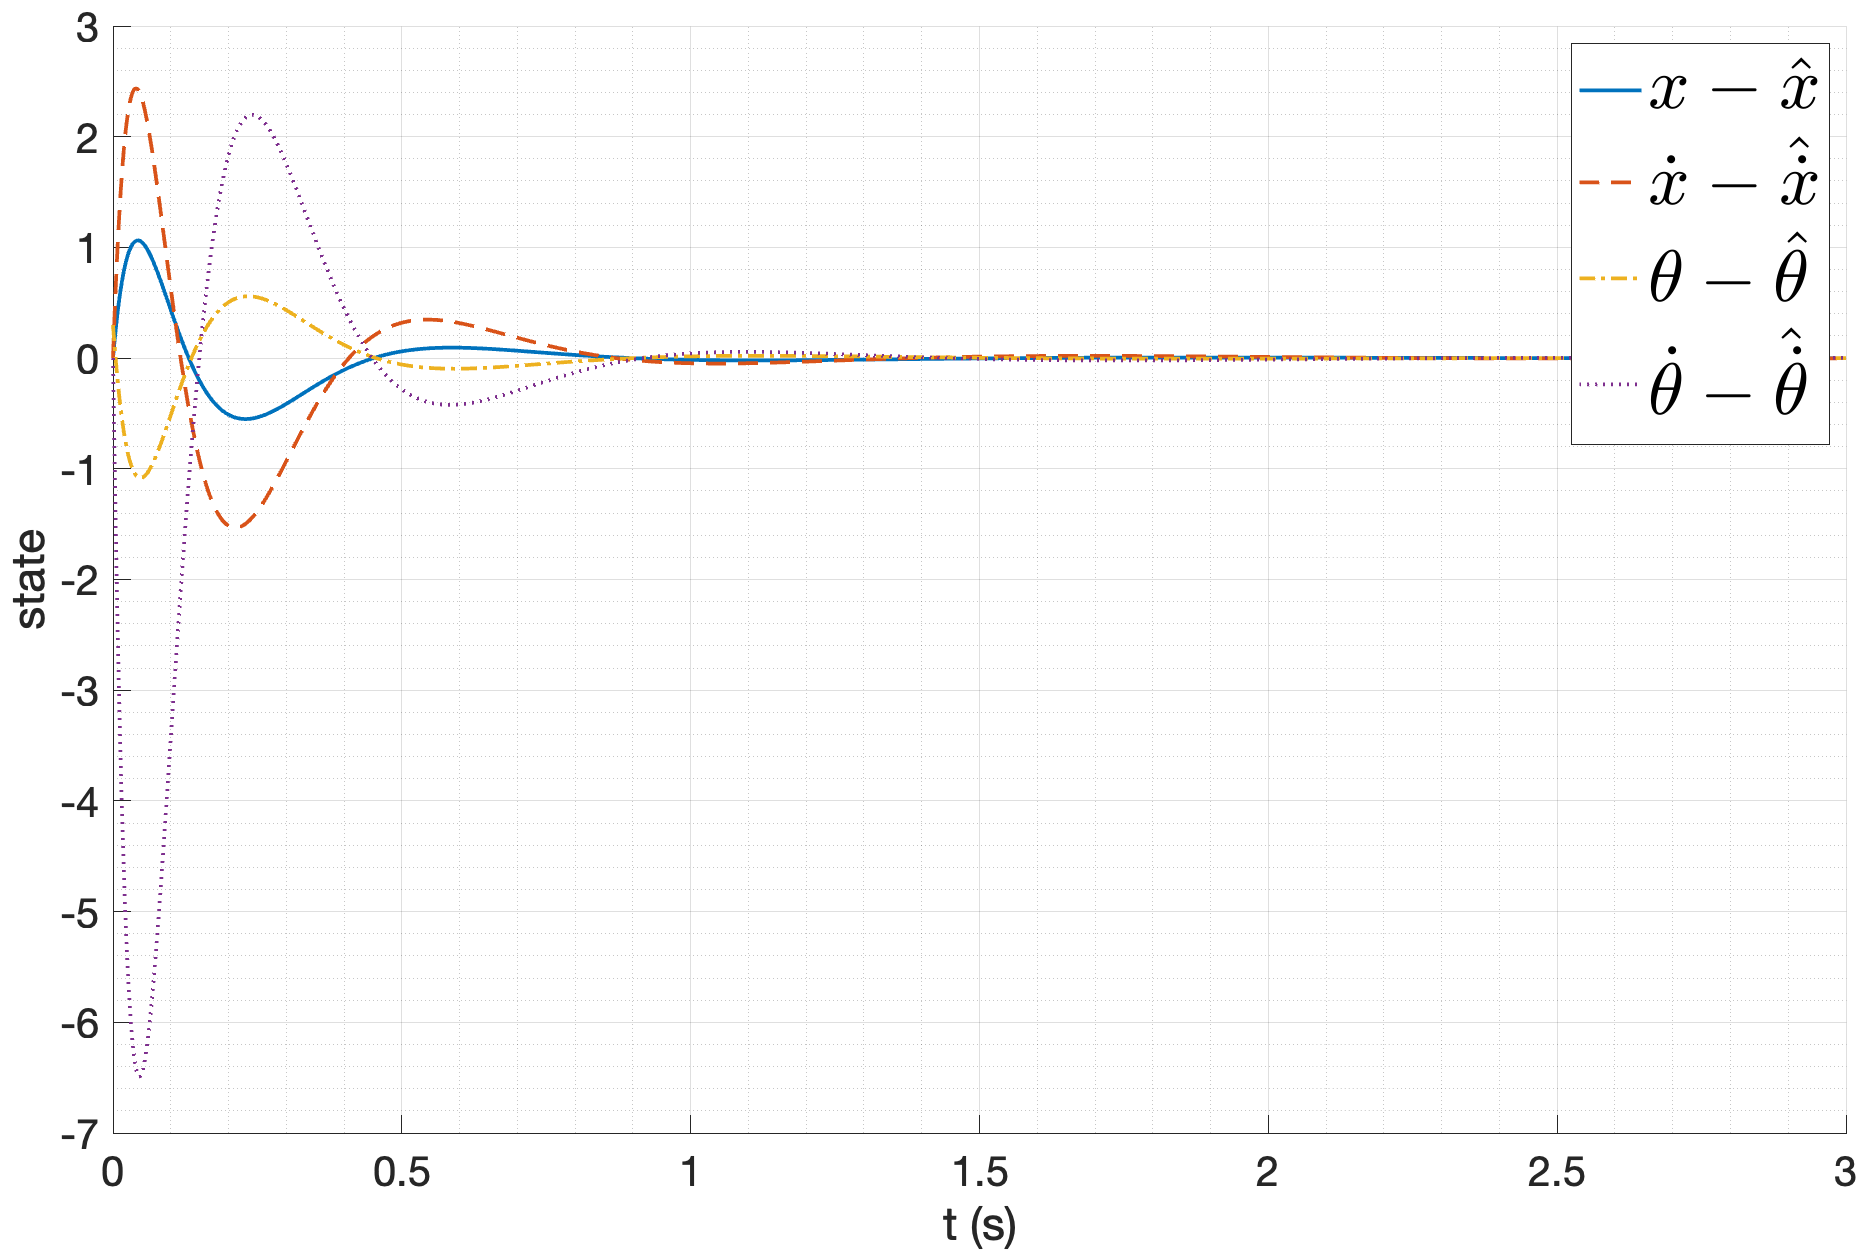
\includegraphics[width=\textwidth]{media/plots/modal_observer/observer_err_2.png}
    \caption{Ошибка оценки состояния системы наблюдателем полного порядка}
    \label{fig:observer_err_2}
\end{figure}
\FloatBarrier
Видно, что теперь время переходного процесса составляет около 1 секунды, что меньше, чем в случае 
наблюдателя с меньшими по модулю собственными числами. 

При этом можно заметить, что начальная ошибка оценки состояния системы увеличилась, особенно сильно это заметно
для оценки угловой скорости маятника. Это может негативно сказаться на работе регулятора, замкнутого по наблюдаемому состоянию.

\subsection{Наблюдатель пониженного порядка}
Так как два значения из вектора состояния являются измеримыми, то можно использовать наблюдатель пониженного порядка, 
который будет оценивать только два оставшихся, неизмеримых состояния системы, которыми являются скорость тележки и угловая скорость маятника.

Рассмотрим наблюдатель пониженного порядка:
\begin{equation}
    \begin{array}{ll}
        \dot{\hat{z}} = \Gamma\hat{z} - Yy + QBu\\
        \hat{x} = \begin{bmatrix}
            C \\ Q
        \end{bmatrix}^{-1} \times \begin{bmatrix}
            y \\ 
            \hat{z}
        \end{bmatrix}
    \end{array}
\end{equation}
Зададим желаемый спектр наблюдателя пониженного порядка $\{-4, -5\}$.

Тогда матрица $Q$ находится из решения уравнения Сильвестра: 
\begin{equation}
   \Gamma Q - QA = YC 
\end{equation}
где $\Gamma$ -- матрица с желаемыми собственными числами. 
Решим уравнение Сильвестра с помощью пакета \texttt{cvx} в MATLAB, в результате получаем матрицу наблюдателя $Q$:
\begin{equation}
    Q = \begin{bmatrix}
    -0.25  & 0.06  & 0.02  & -0.00 \\ 
    -0.20  & 0.04  & -0.01  & 0.00 \\
    \end{bmatrix}
\end{equation}

Схема наблюдателя пониженного порядка приведена на рисунке \ref{fig:reduced_observer_scheme}.
\begin{figure}[ht!]
    \centering
    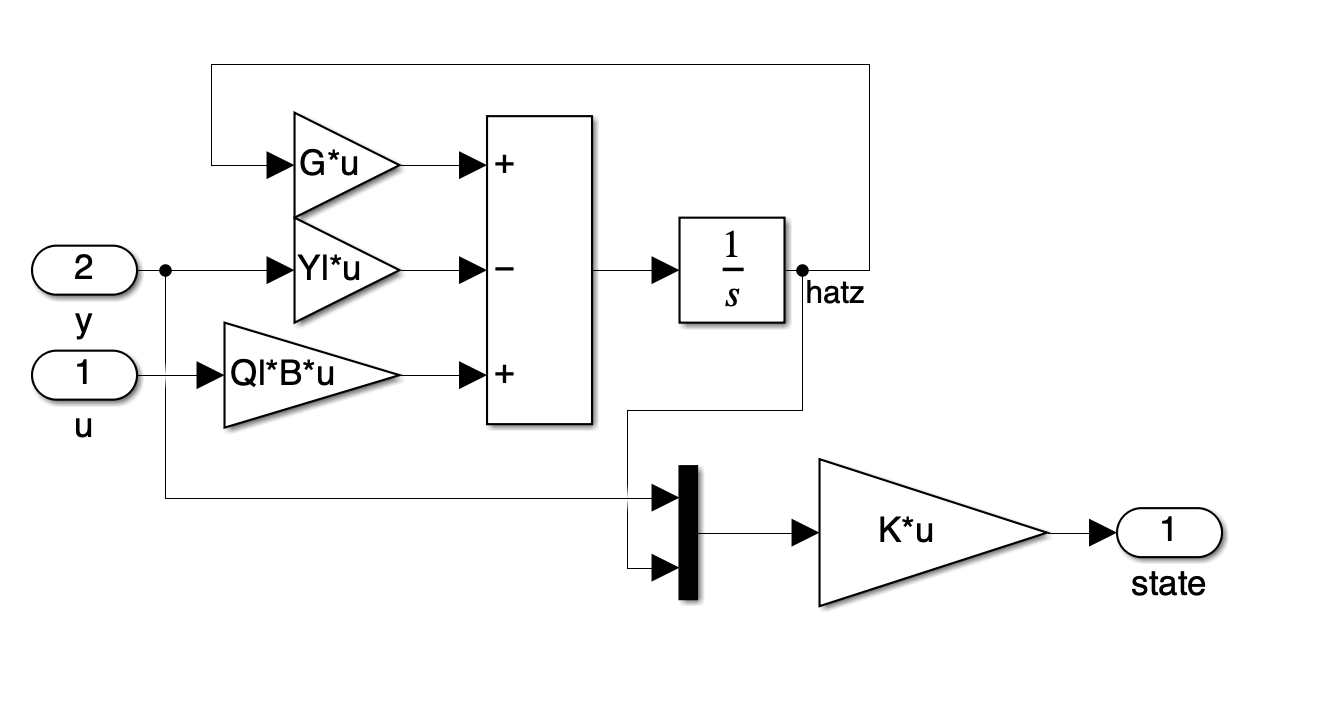
\includegraphics[width=0.7\textwidth]{media/reduced_observer_scheme.png}
    \caption{Схема наблюдателя пониженного порядка}
    \label{fig:reduced_observer_scheme}
\end{figure}

Схема включения наблюдателя в систему аналогичная схеме включения наблюдателя полного порядка, 
которая приведена на рисунке \ref{fig:observer_system}. 

Проверим работу наблюдателя пониженного порядка, сравнив его выход с реальным состоянием нелинейной системы.
Результаты моделирования приведены на рисунке \ref{fig:reduced_observer_x_1} и рисунках \ref{fig:reduced_observer_x_cmp_1_sep}.
\begin{figure}[ht!]
    \centering
    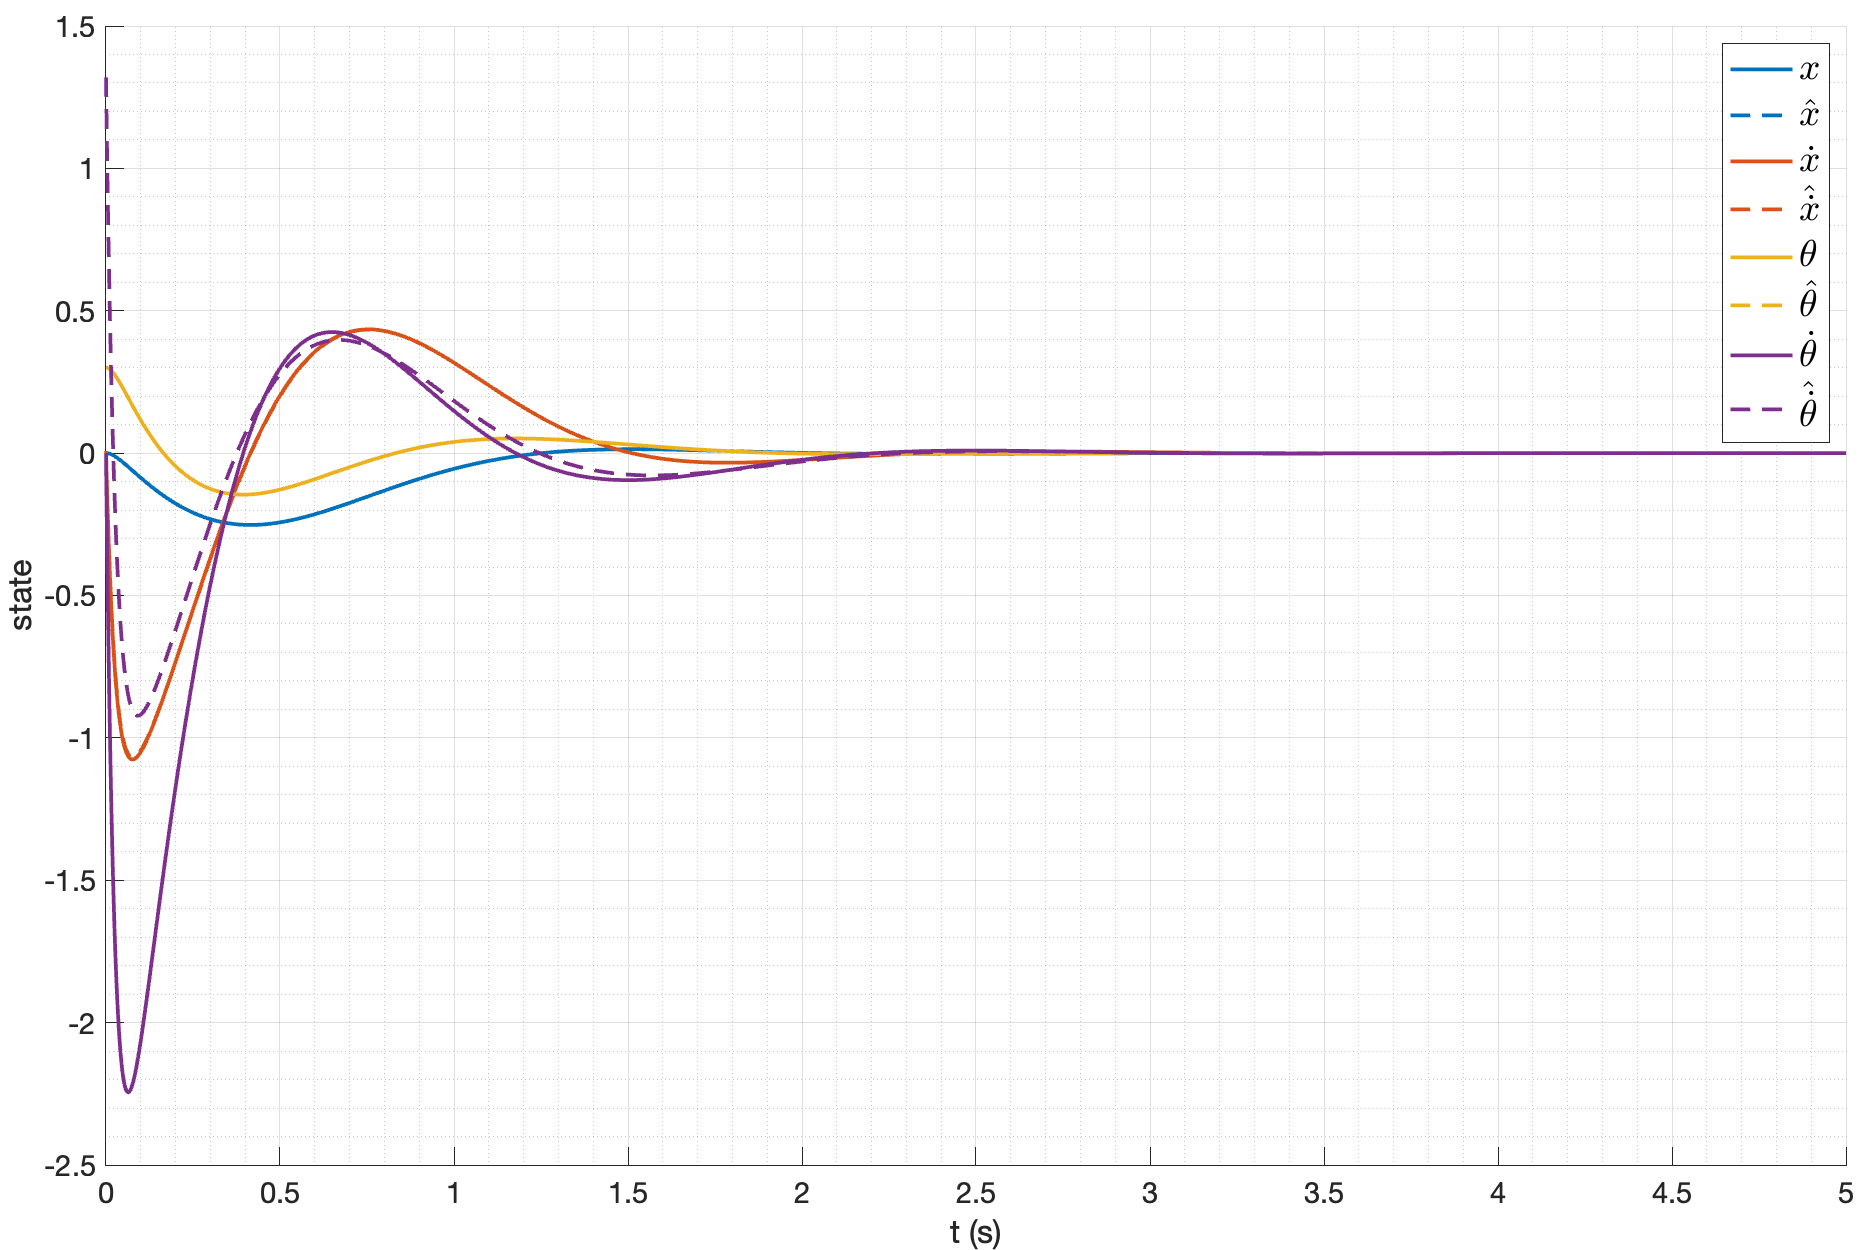
\includegraphics[width=\textwidth]{media/plots/reduced_observer/reduced_observer_cmp_1.png}
    \caption{Результаты моделирования наблюдателя пониженного порядка}
    \label{fig:reduced_observer_x_1}
\end{figure}

\begin{figure}[ht!]
    \centering
    \begin{subfigure}[b]{0.45\textwidth}
        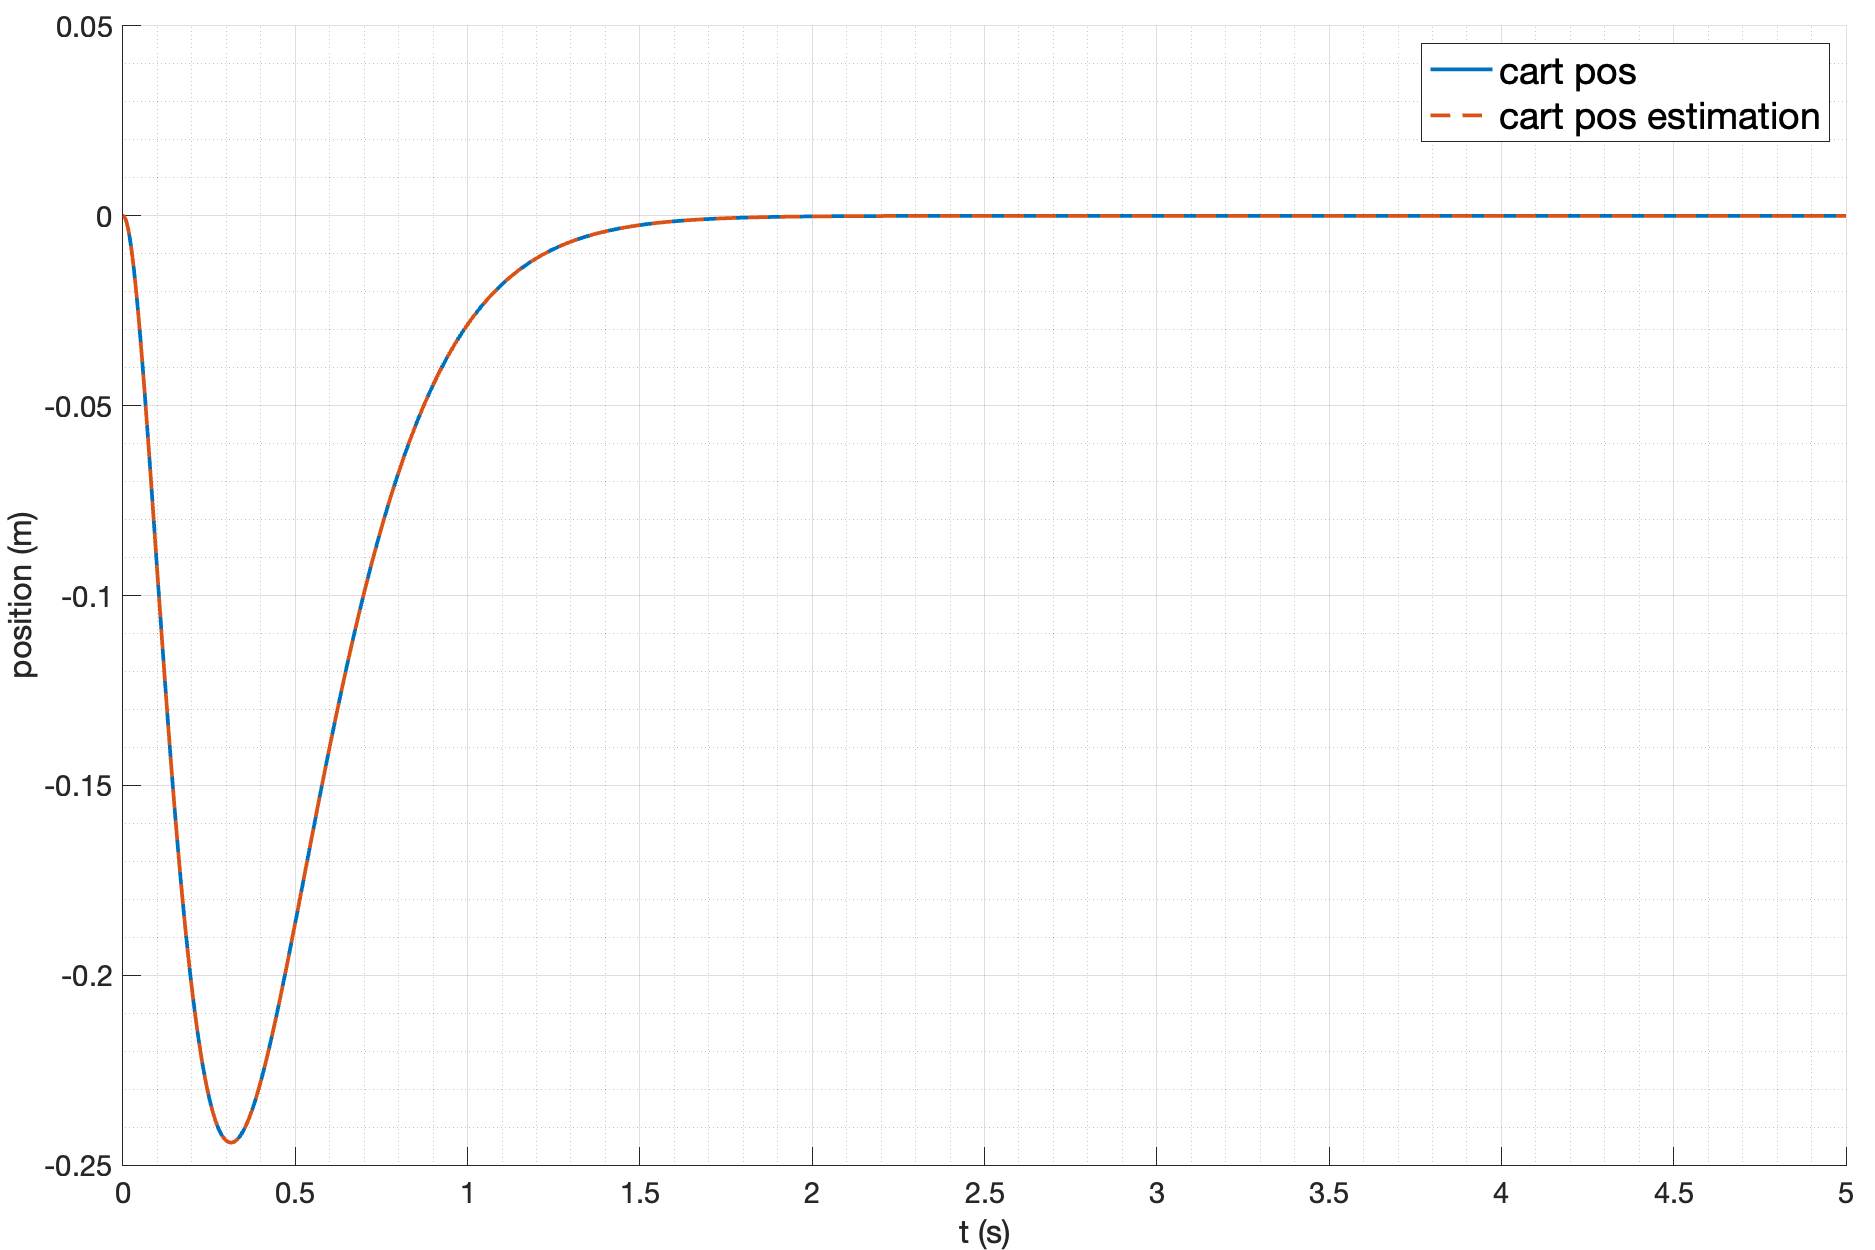
\includegraphics[width=\textwidth]{media/plots/reduced_observer/reduced_observer_x_cmp_1.png}
        \caption{Оценка координаты тележки}
        \label{fig:reduced_observer_x_cmp_1}
    \end{subfigure}
    \begin{subfigure}[b]{0.45\textwidth}
        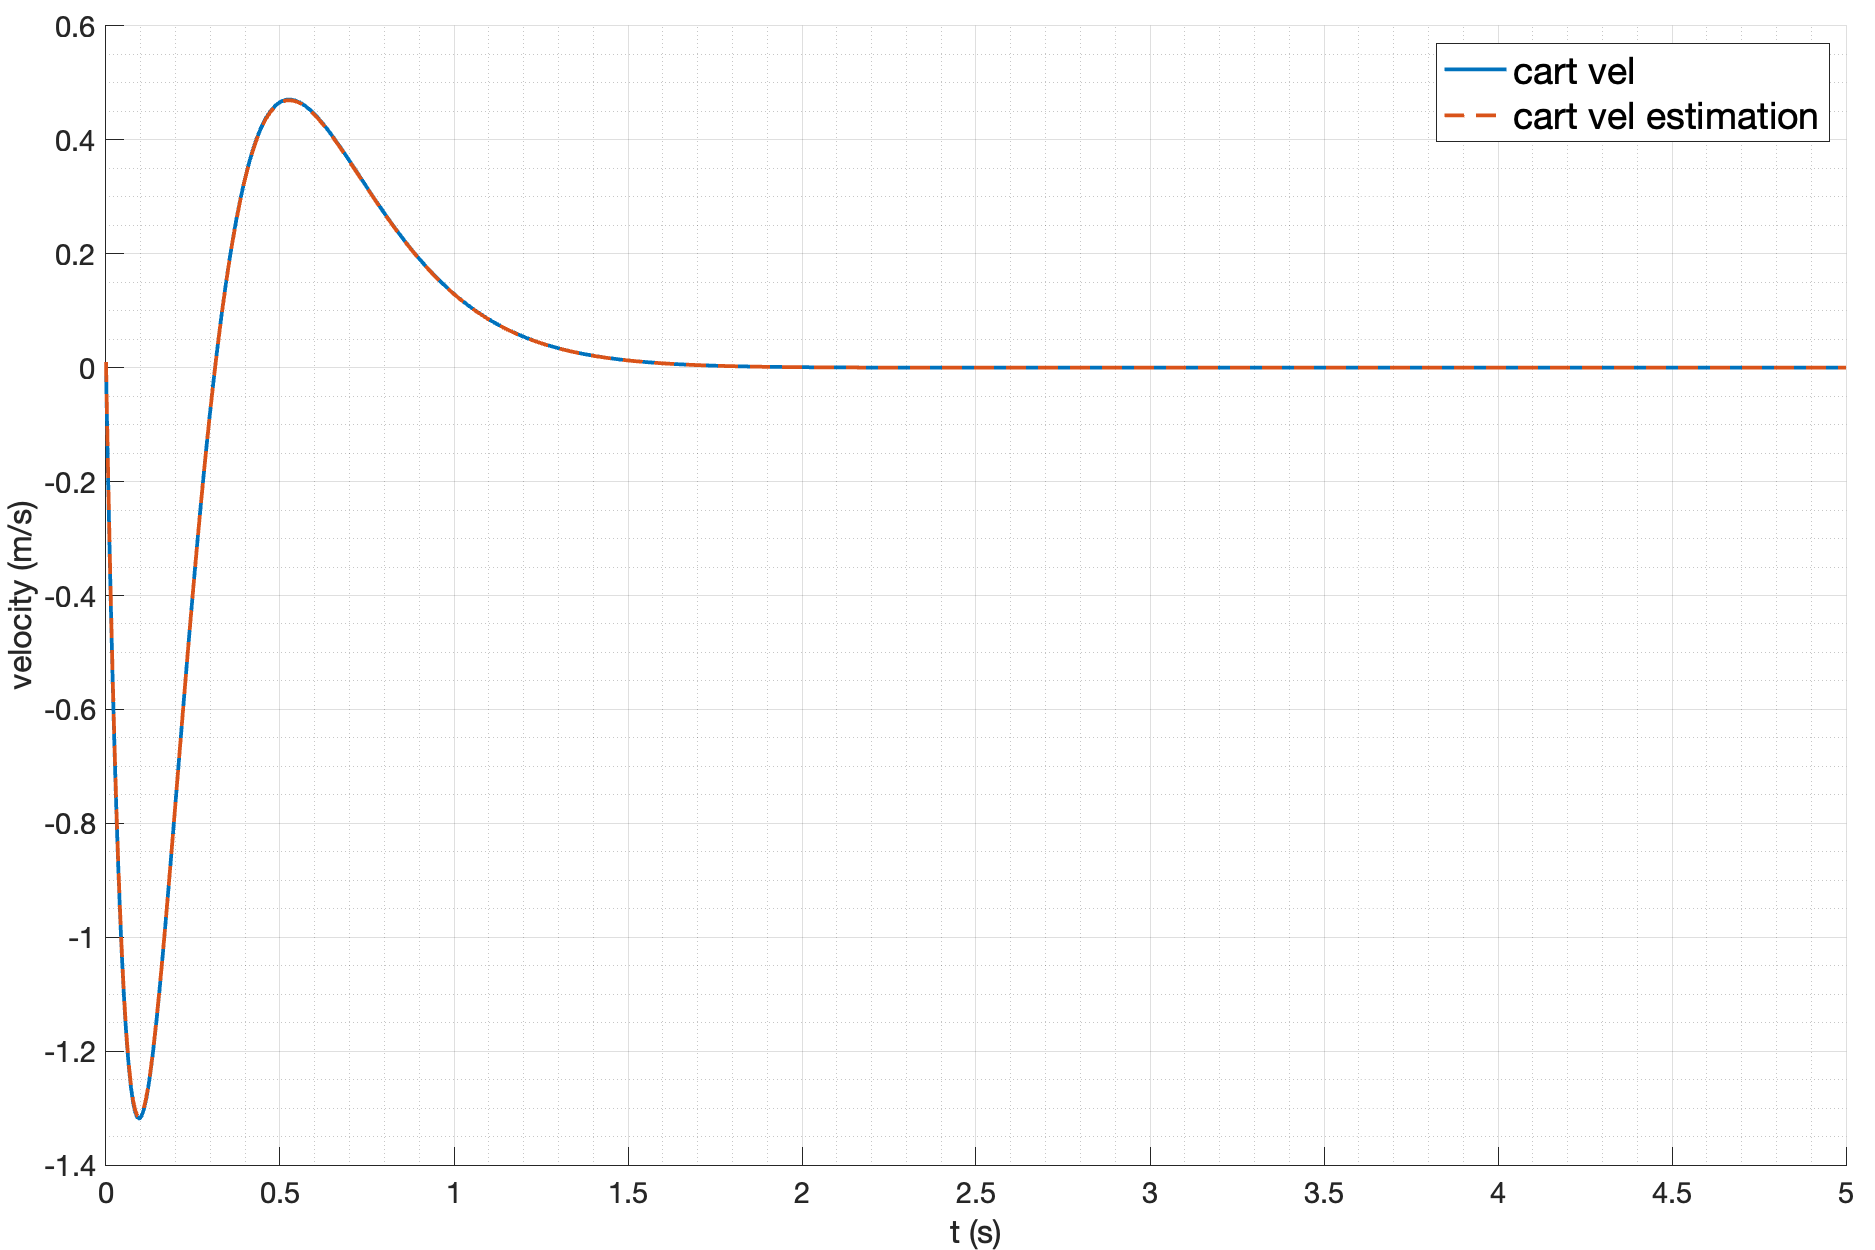
\includegraphics[width=\textwidth]{media/plots/reduced_observer/reduced_observer_dotx_cmp_1.png}
        \caption{Оценка скорости тележки}
        \label{fig:reduced_observer_dotx_cmp_1}
    \end{subfigure}
    \begin{subfigure}[b]{0.45\textwidth}
        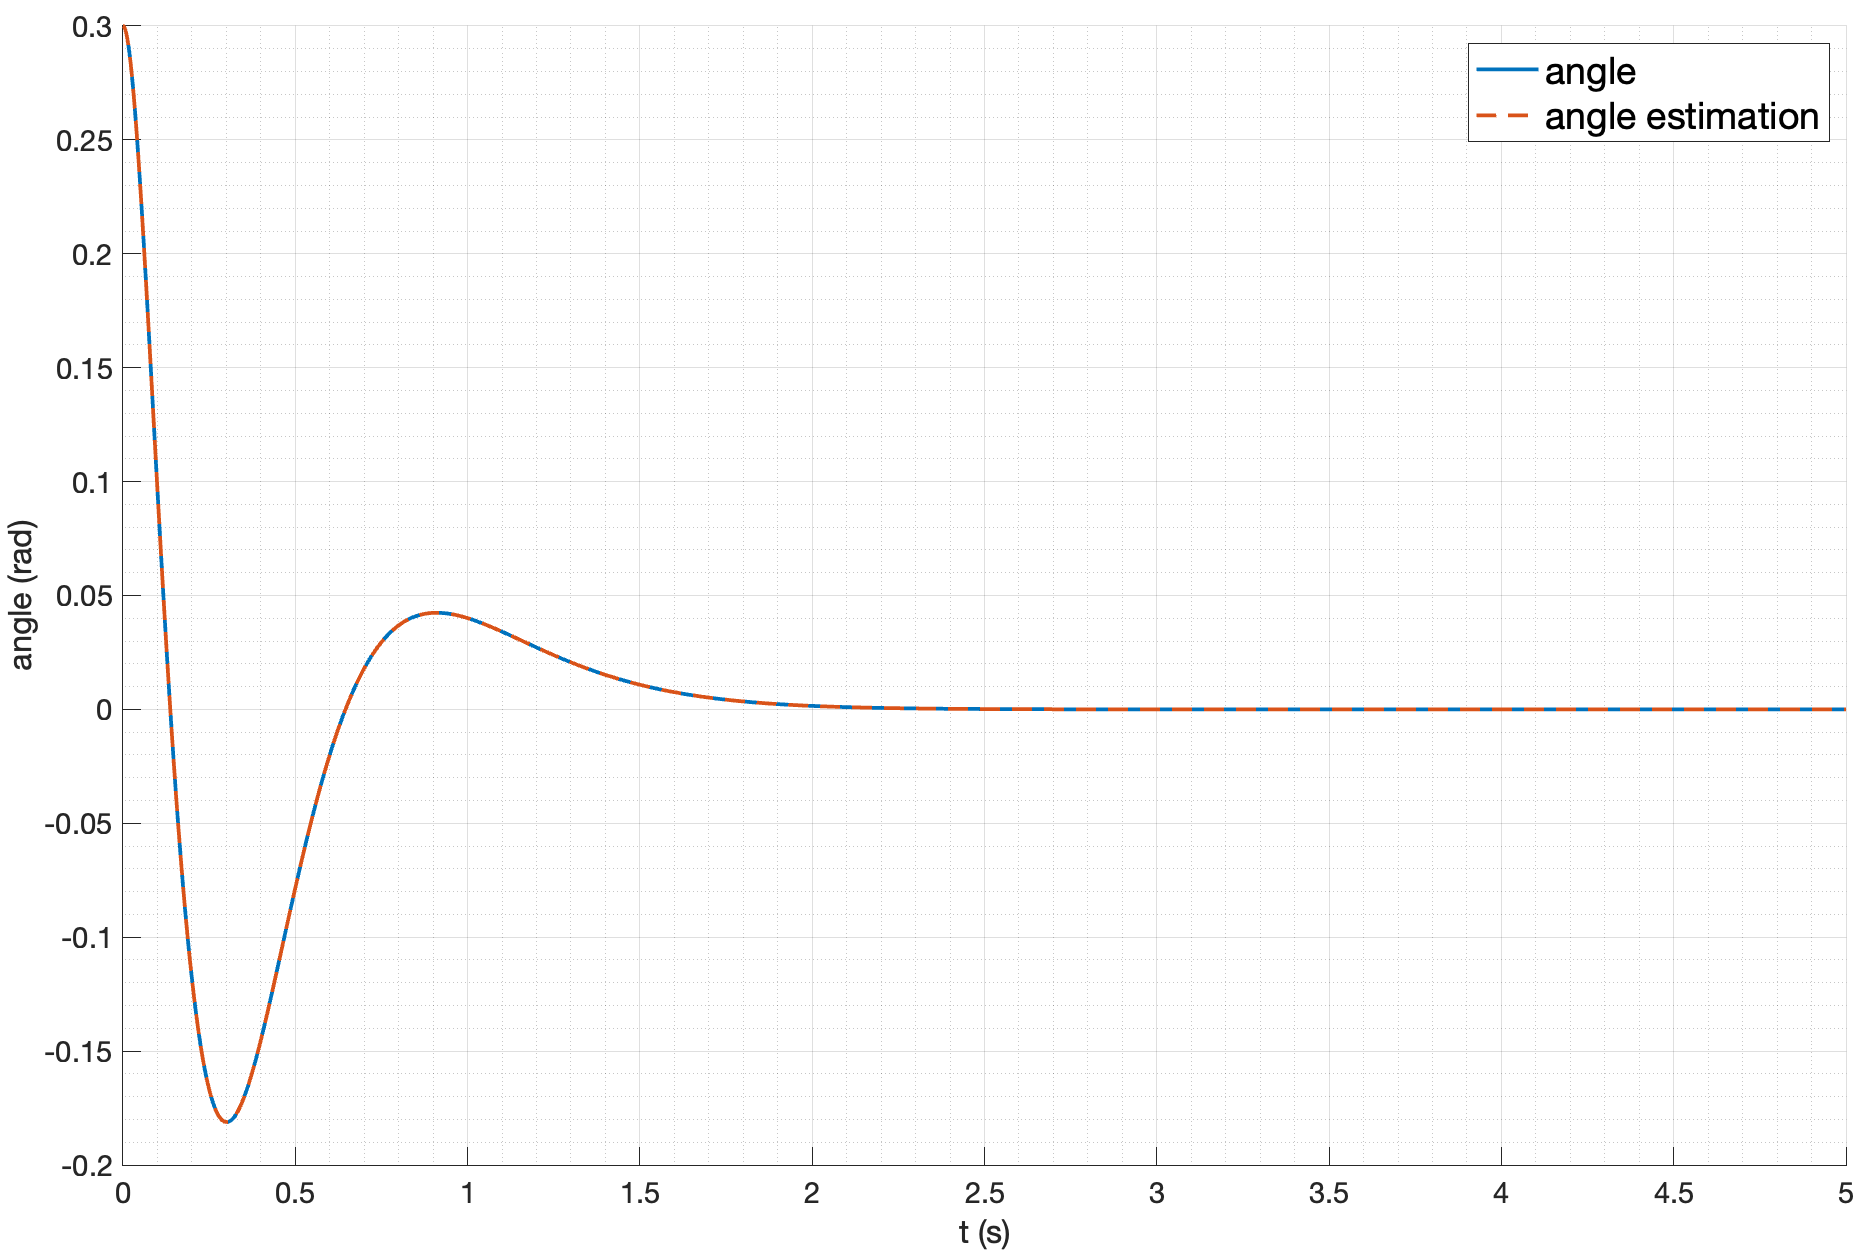
\includegraphics[width=\textwidth]{media/plots/reduced_observer/reduced_observer_theta_cmp_1.png}
        \caption{Оценка угла отклонения маятника}
        \label{fig:reduced_observer_theta_cmp_1}
    \end{subfigure}
    \begin{subfigure}[b]{0.45\textwidth}
        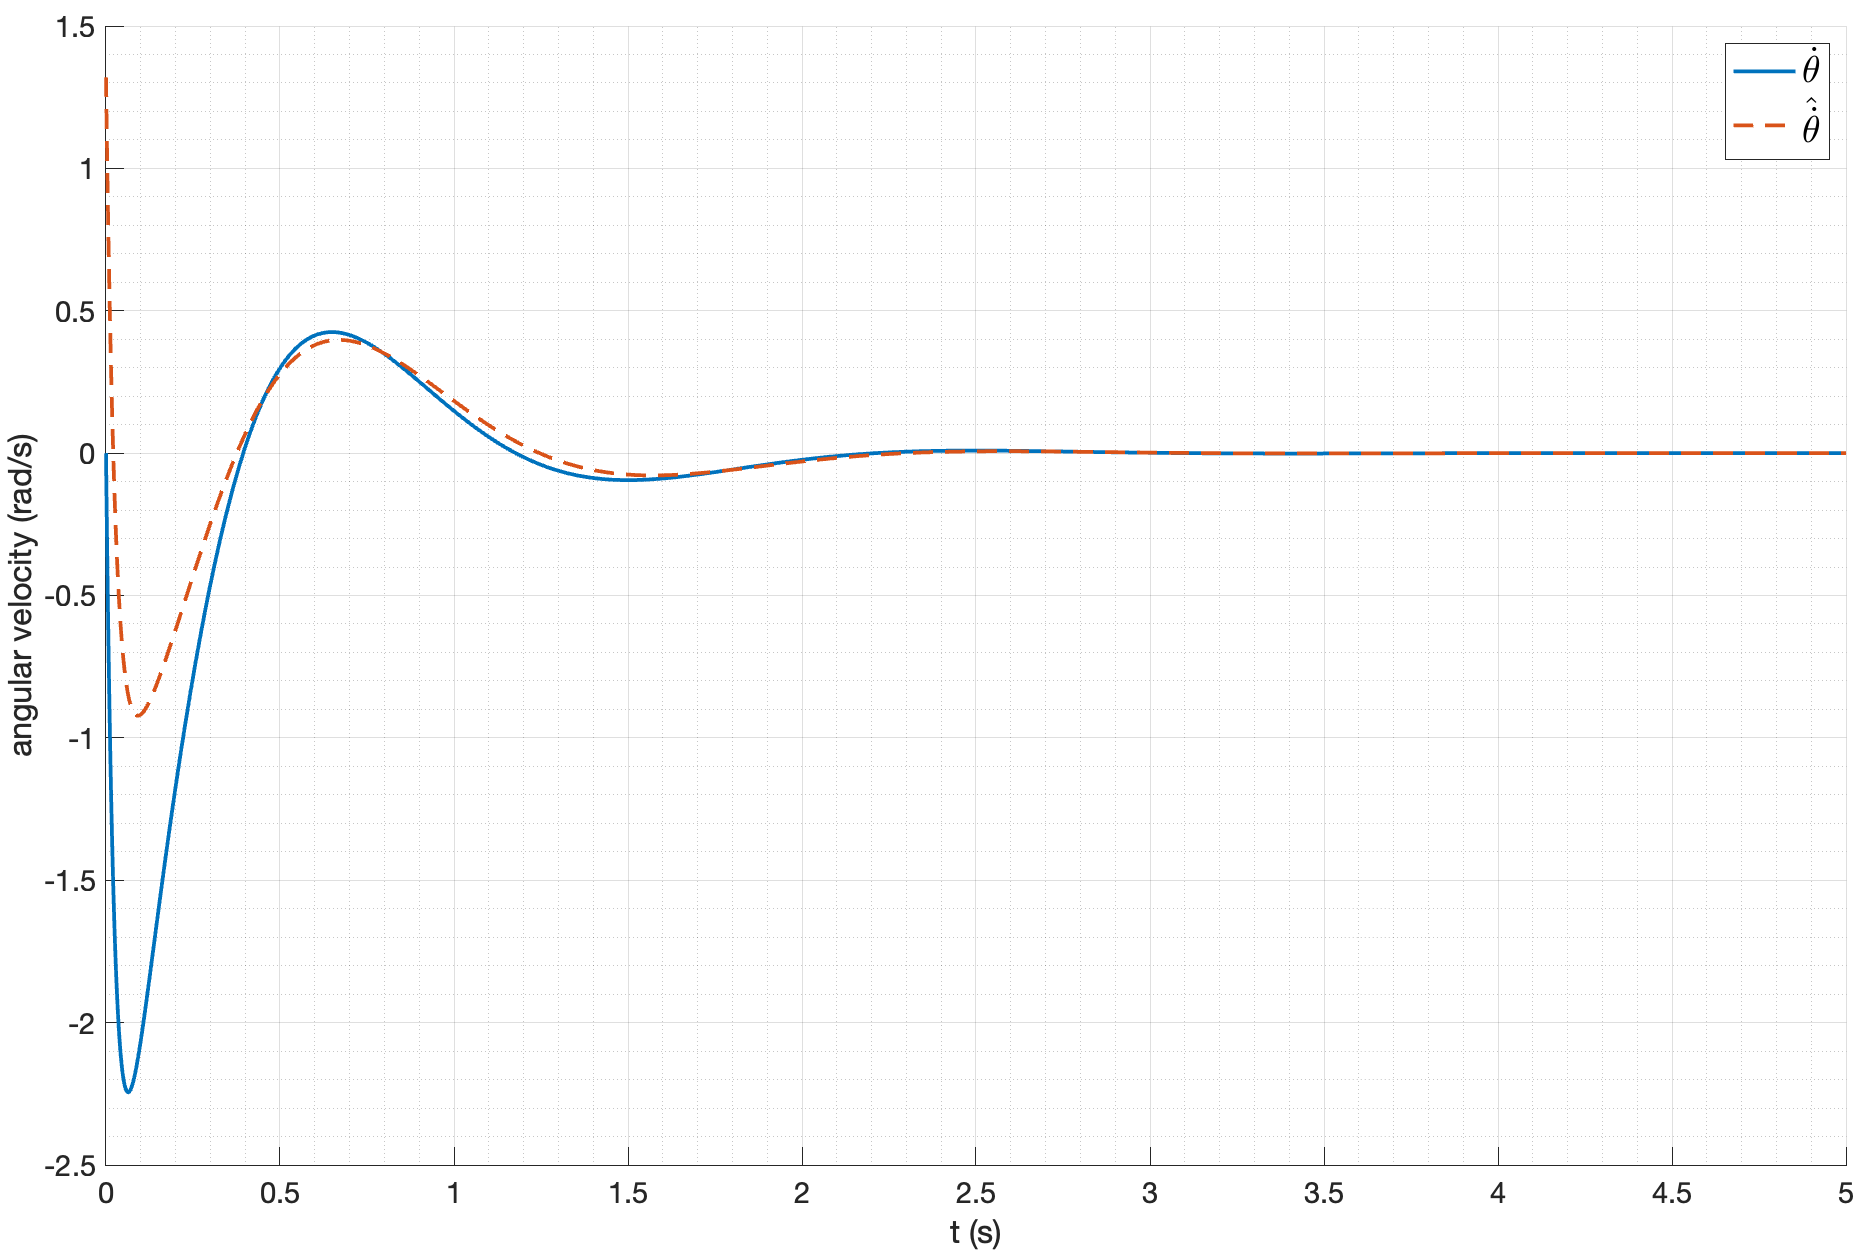
\includegraphics[width=\textwidth]{media/plots/reduced_observer/reduced_observer_dottheta_cmp_1.png}
        \caption{Оценка угловой скорости маятника}
        \label{fig:reduced_observer_dottheta_cmp_1}
    \end{subfigure}
    \caption{Сравнение оценок состояния системы с реальным состоянием наблюдателем пониженного порядка}
    \label{fig:reduced_observer_x_cmp_1_sep}
\end{figure}
Ошибка оценки состояния системы приведена на рисунке \ref{fig:reduced_observer_err_1}.
\begin{figure}[ht!]
    \centering
    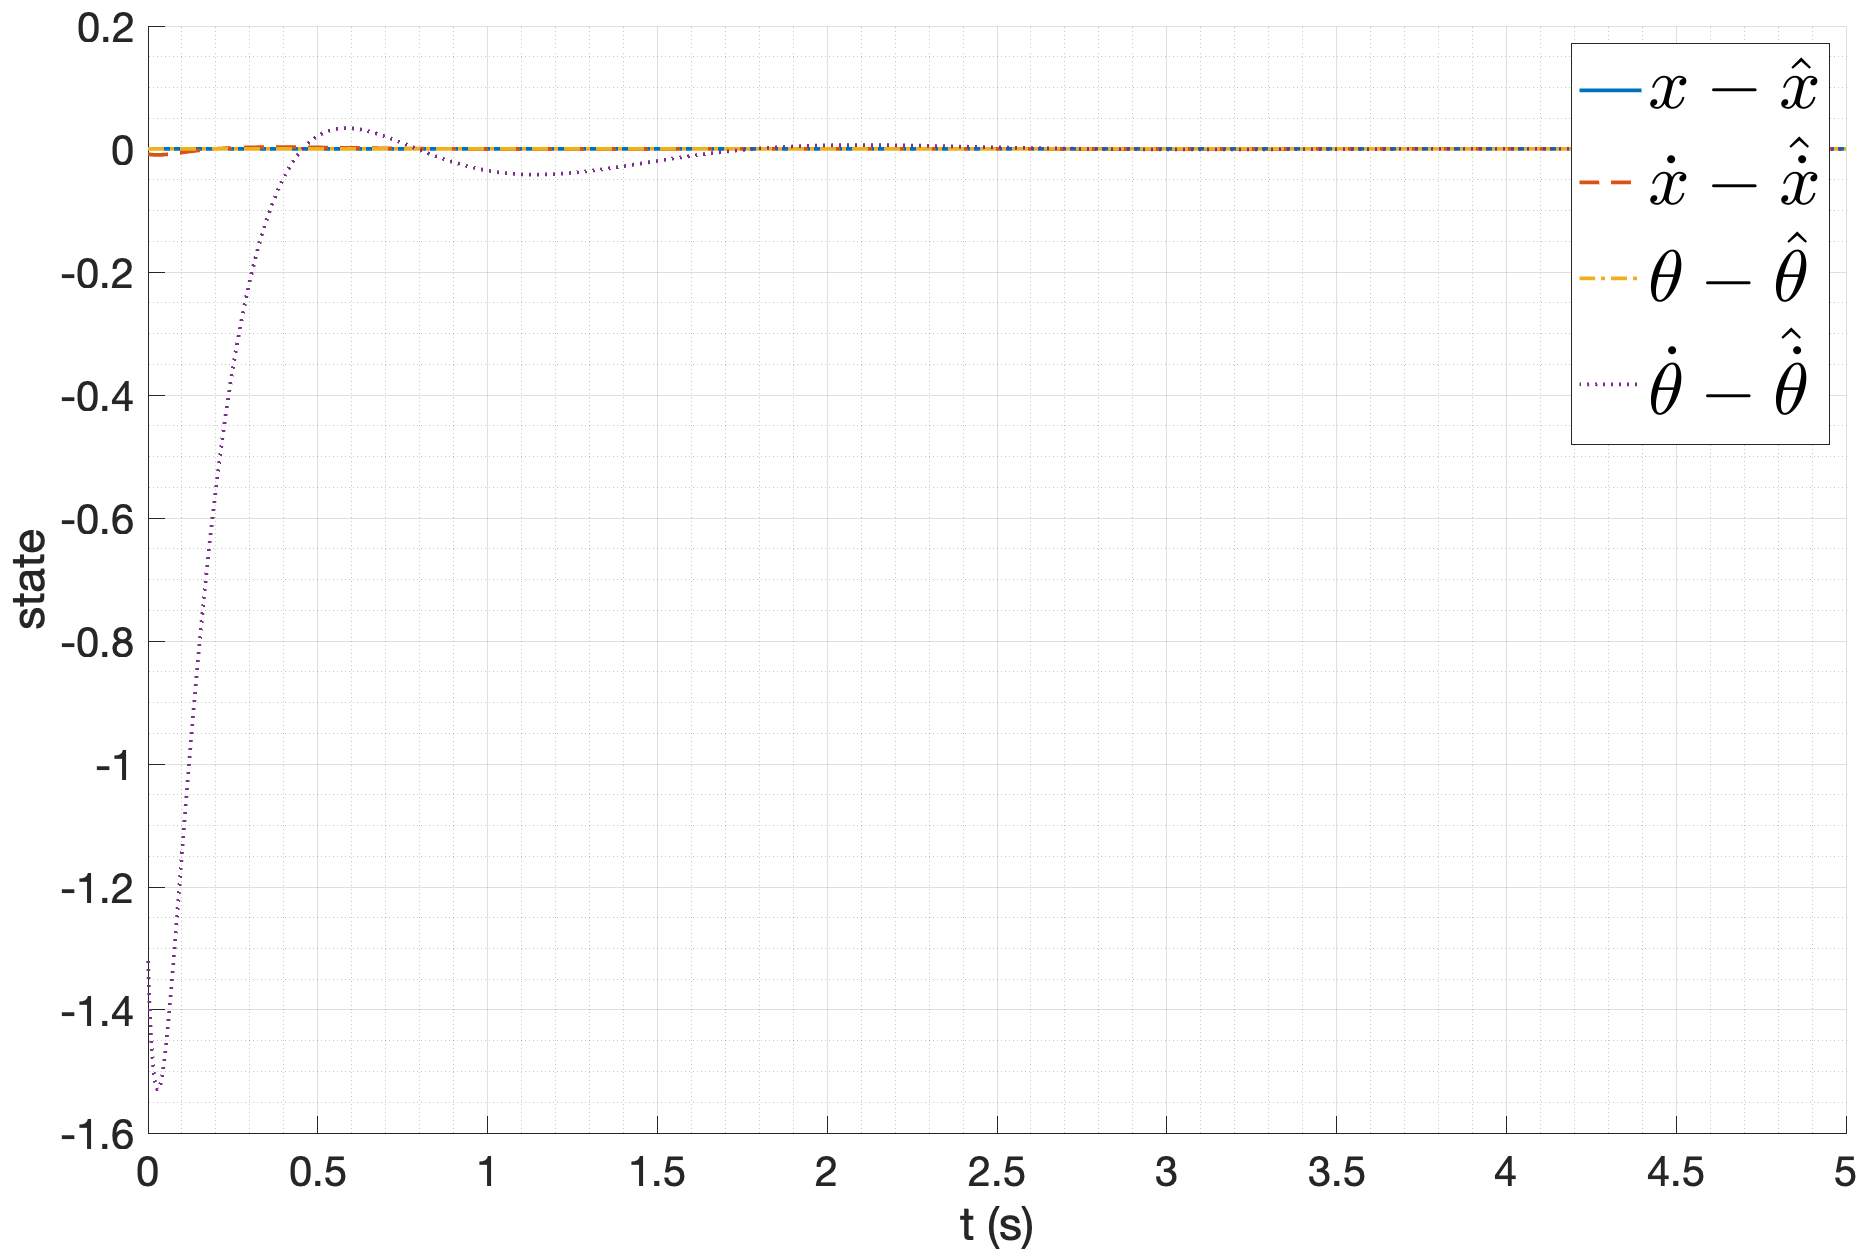
\includegraphics[width=\textwidth]{media/plots/reduced_observer/reduced_observer_err_1.png}
    \caption{Ошибка оценки состояния системы наблюдателем пониженного порядка}
    \label{fig:reduced_observer_err_1}
\end{figure}
\FloatBarrier
Видно, что оценка состояния нелинейной системы наблюдателем пониженного порядка 
не отличается от реального состояния системы для координаты тележки и угла отклонения маятника,
так как они являются напрямую измеримыми. При этом оценка скорости тележки и угловой скорости
маятника тоже сходится к реальным значениям. Время переходного процесса составляет около 1 секунды.

Рассмотрим наблюдатель пониженного порядка с желаемым спектром $\{-1, -1\}$.
Результаты моделирования приведены на рисунке \ref{fig:reduced_observer_x_2} и рисунках \ref{fig:reduced_observer_x_cmp_2_sep}.
\begin{figure}[ht!]
    \centering
    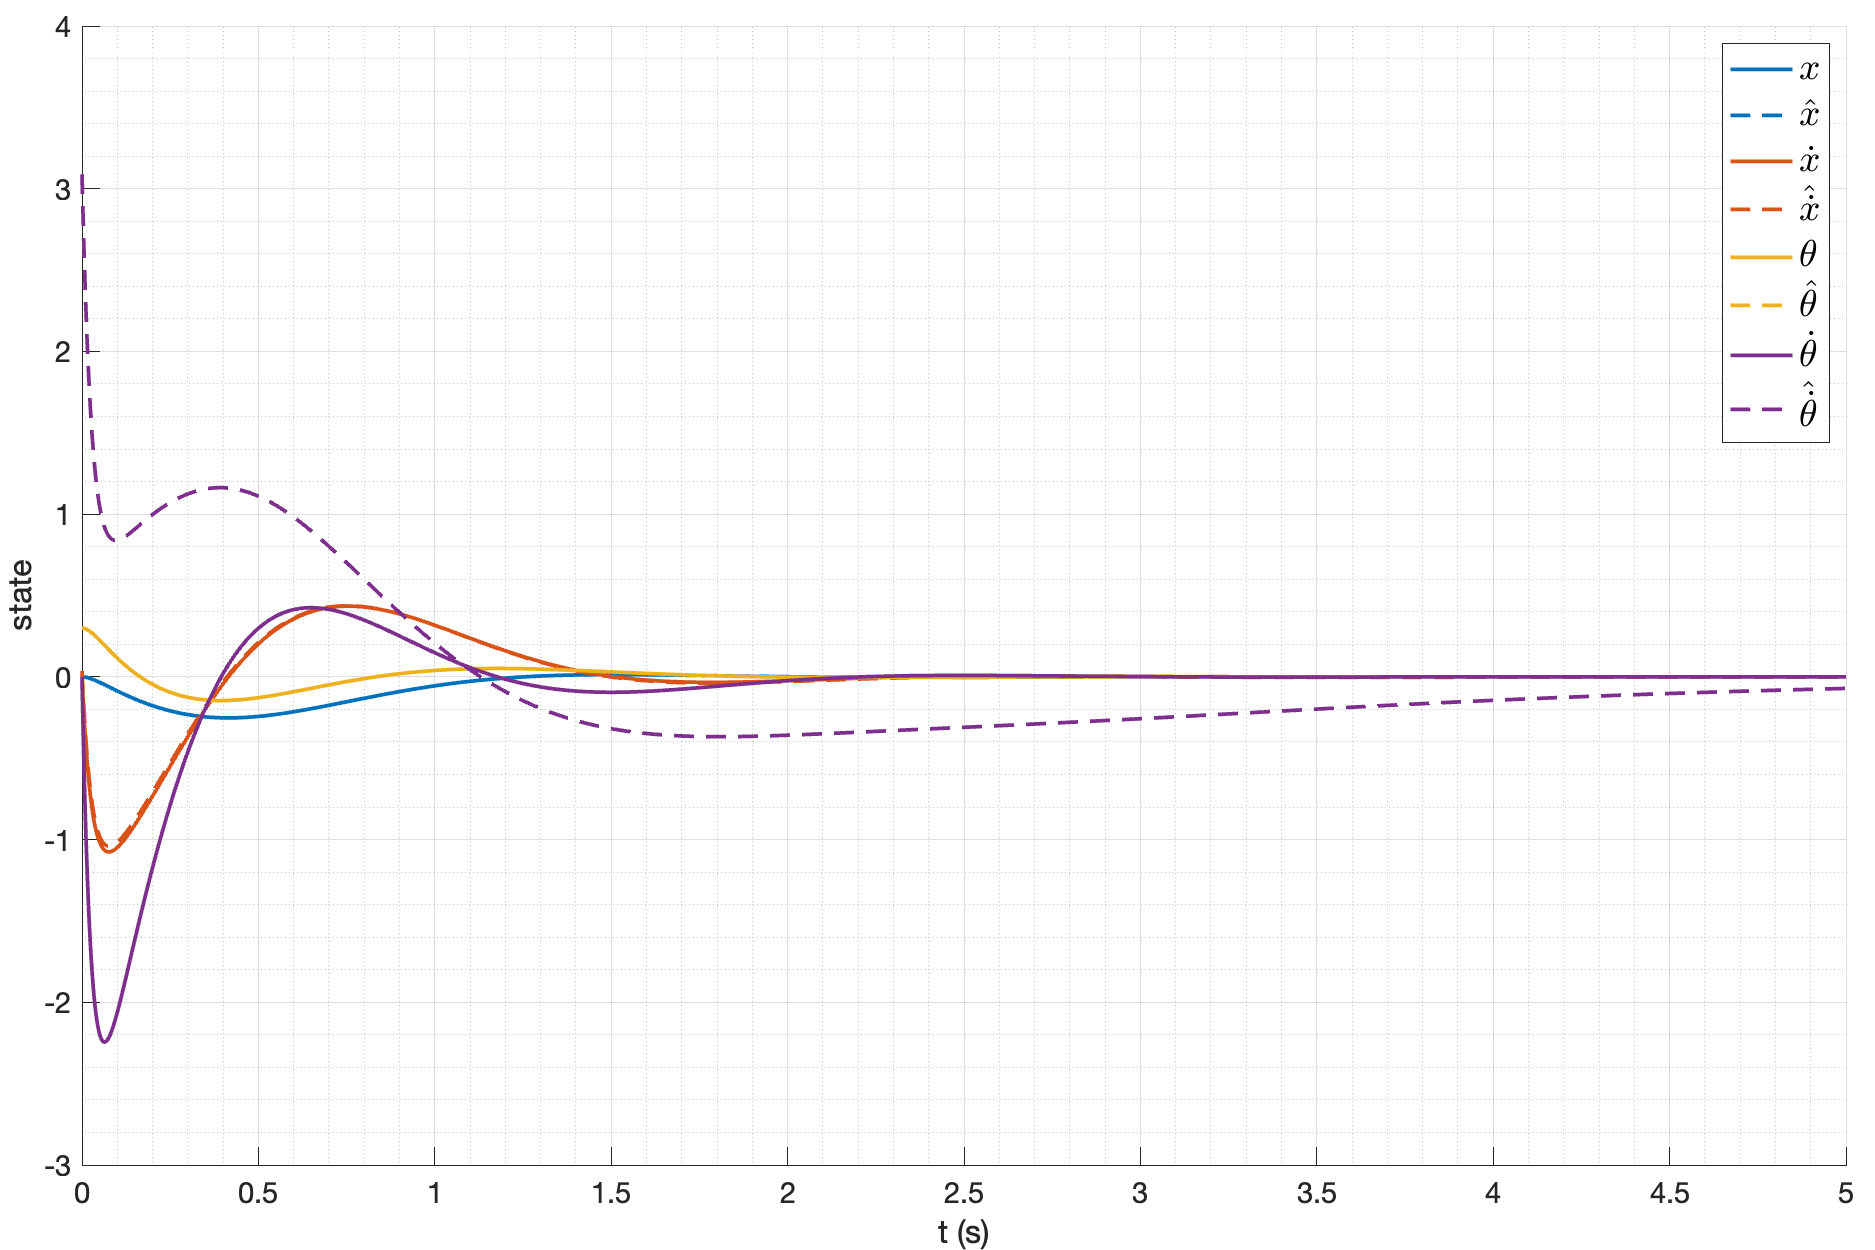
\includegraphics[width=\textwidth]{media/plots/reduced_observer/reduced_observer_cmp_2.png}
    \caption{Результаты моделирования наблюдателя пониженного порядка}
    \label{fig:reduced_observer_x_2}
\end{figure}
\begin{figure}[ht!]
    \centering
    \begin{subfigure}[b]{0.45\textwidth}
        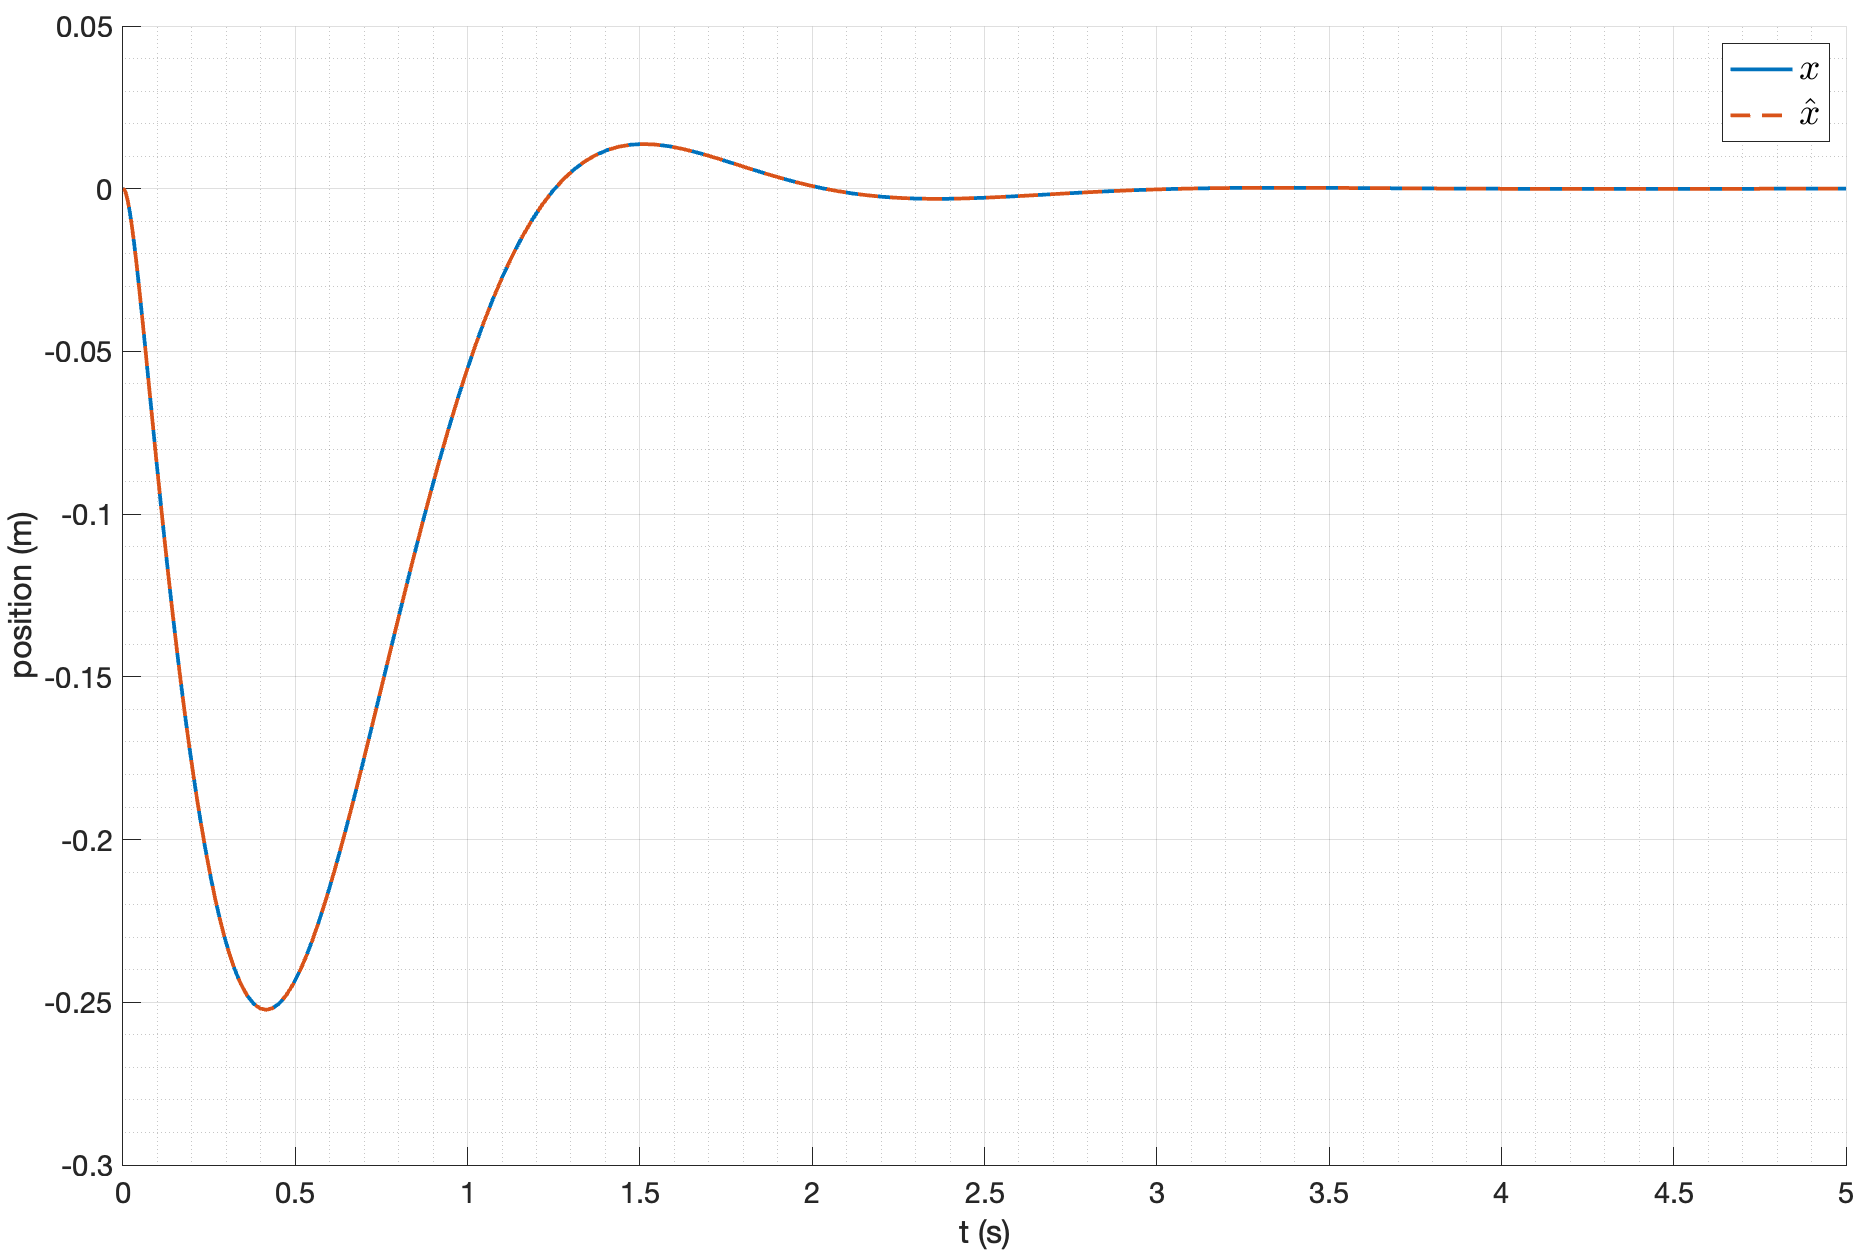
\includegraphics[width=\textwidth]{media/plots/reduced_observer/reduced_observer_x_cmp_2.png}
        \caption{Оценка координаты тележки}
        \label{fig:reduced_observer_x_cmp_2}
    \end{subfigure}
    \begin{subfigure}[b]{0.45\textwidth}
        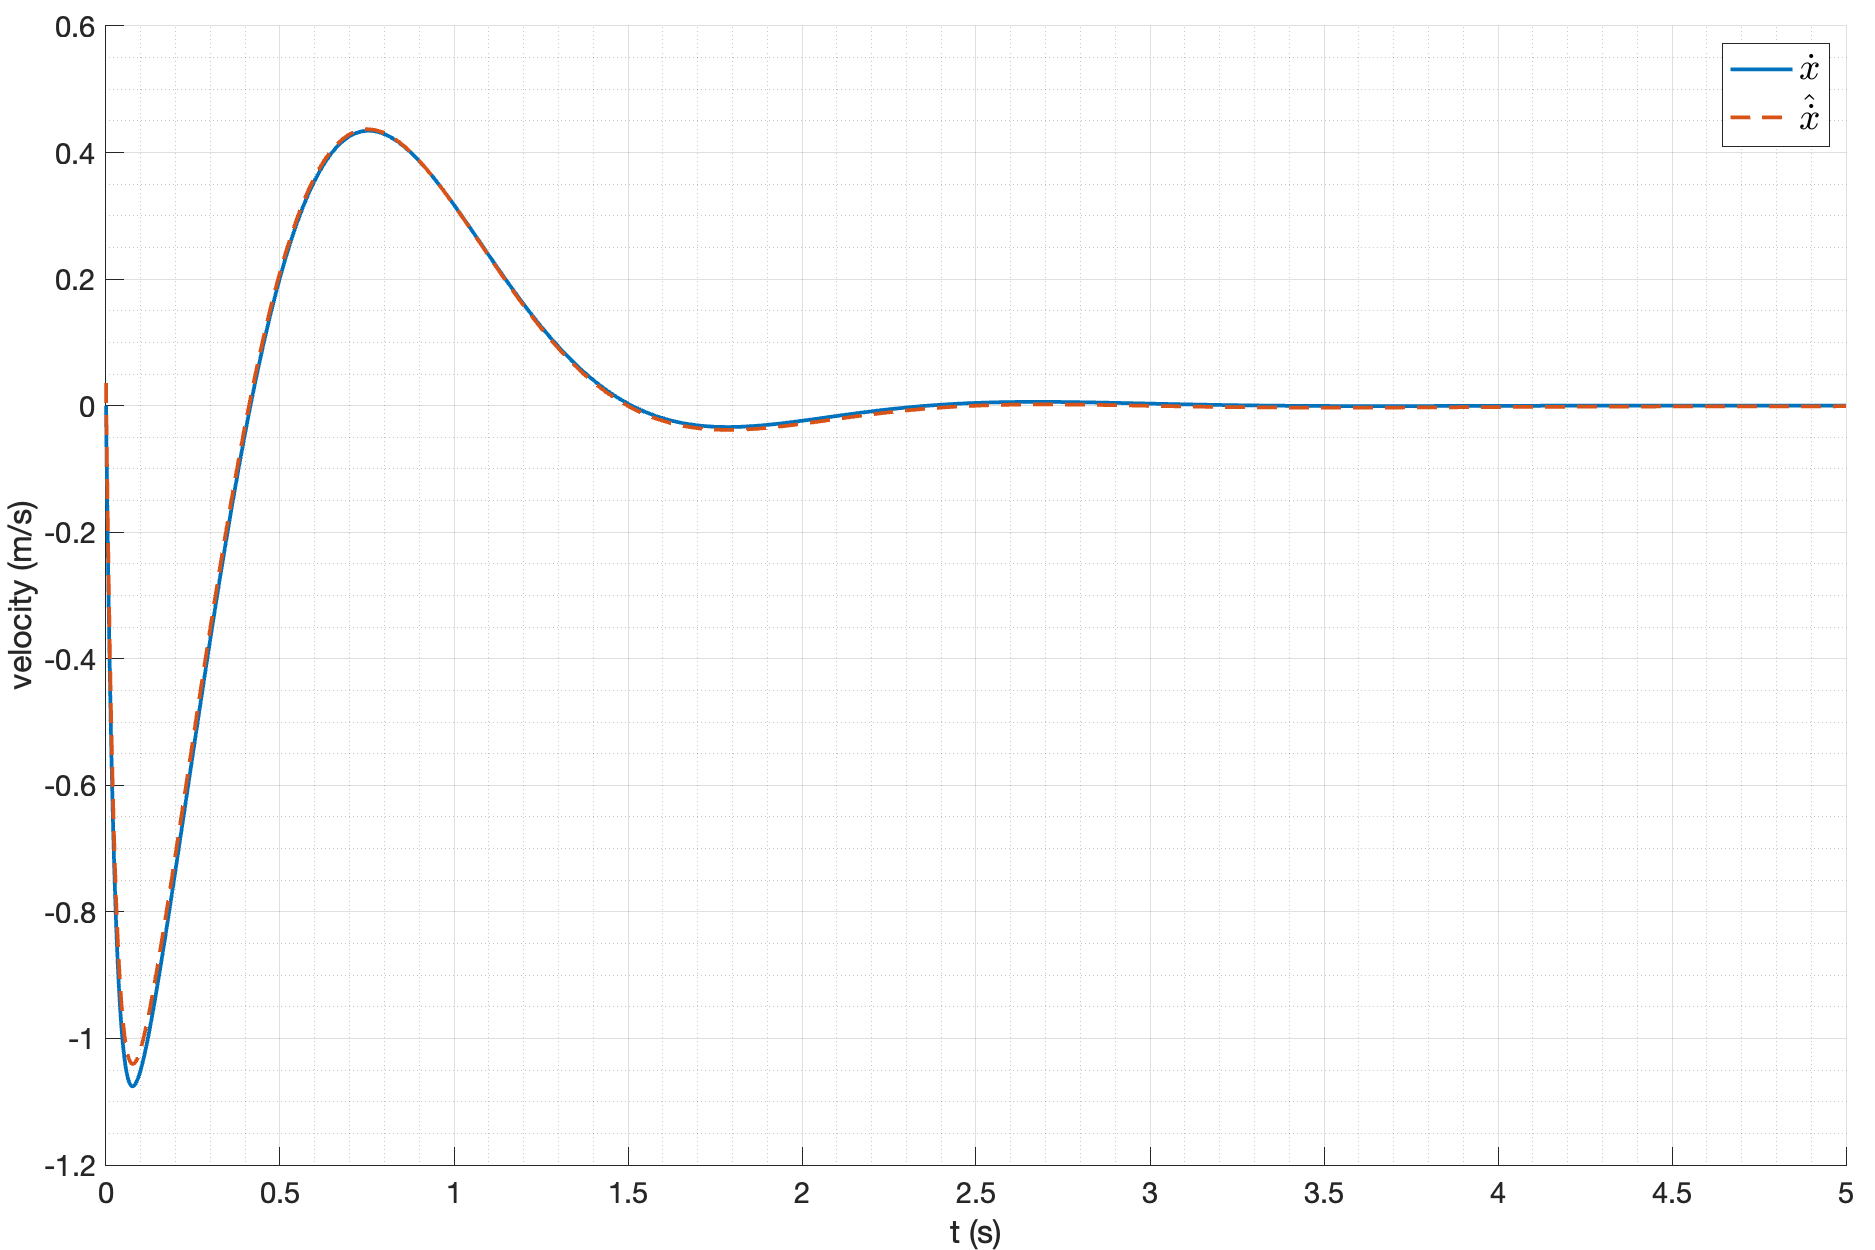
\includegraphics[width=\textwidth]{media/plots/reduced_observer/reduced_observer_dotx_cmp_2.png}
        \caption{Оценка скорости тележки}
        \label{fig:reduced_observer_dotx_cmp_2}
    \end{subfigure}
    \begin{subfigure}[b]{0.45\textwidth}
        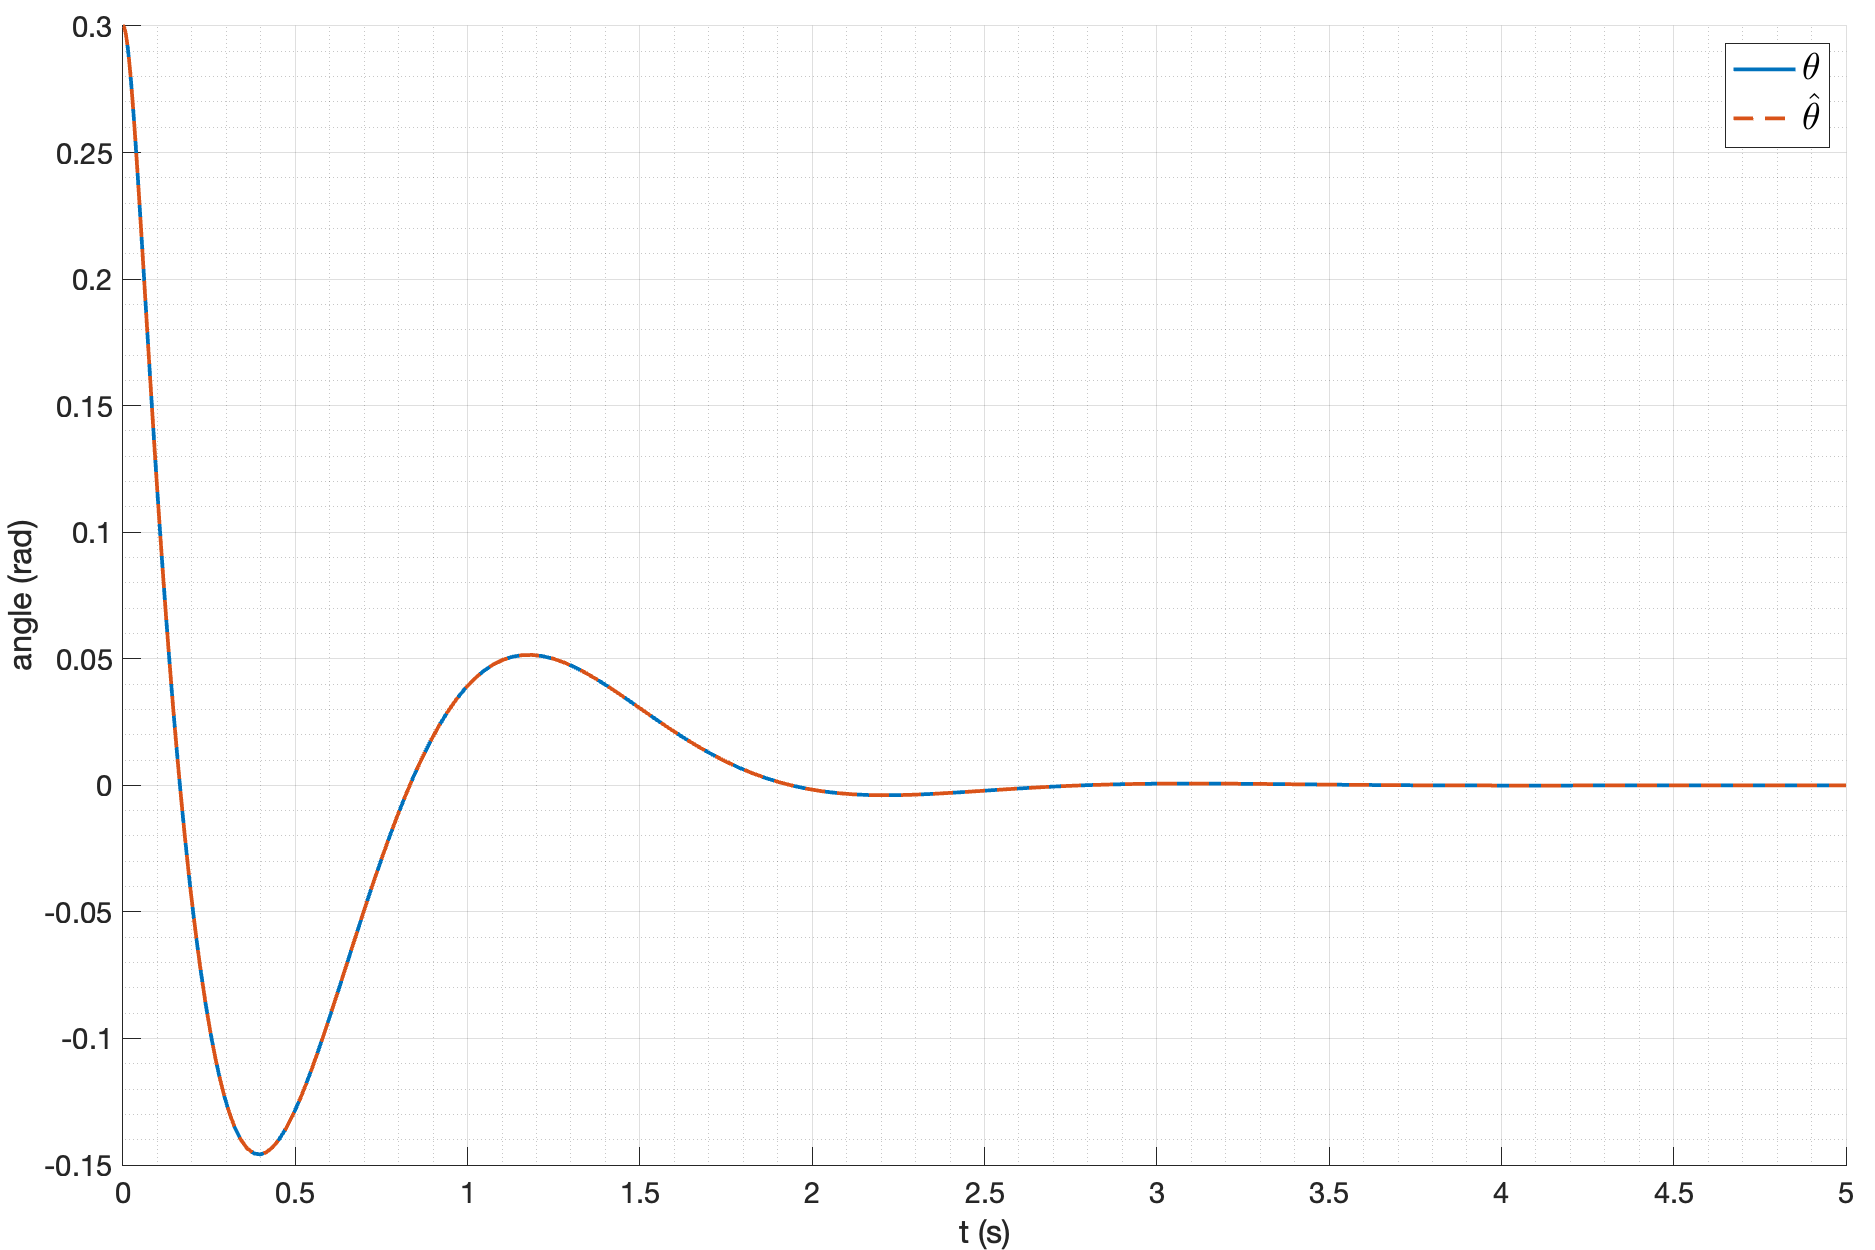
\includegraphics[width=\textwidth]{media/plots/reduced_observer/reduced_observer_theta_cmp_2.png}
        \caption{Оценка угла отклонения маятника}
        \label{fig:reduced_observer_theta_cmp_2}
    \end{subfigure}
    \begin{subfigure}[b]{0.45\textwidth}
        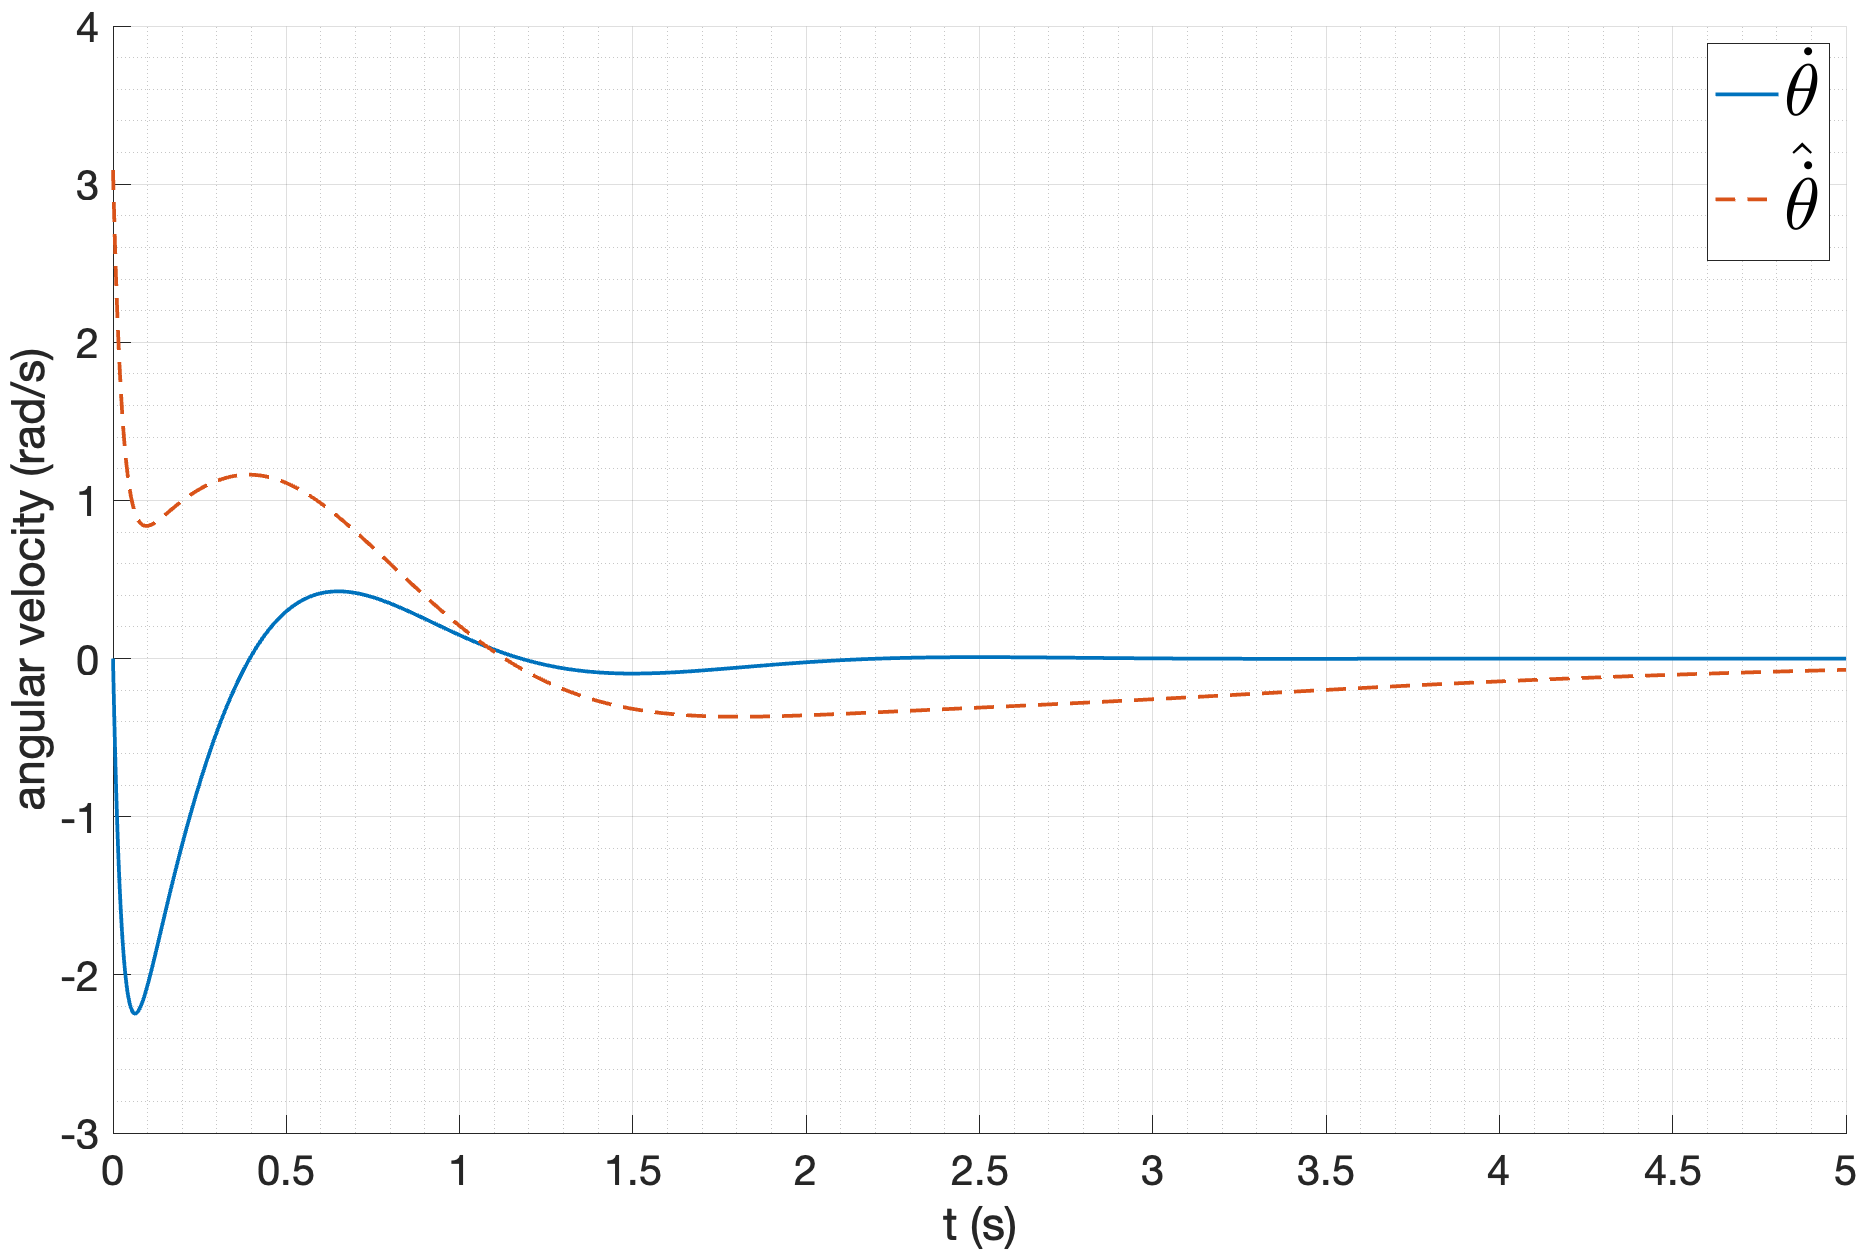
\includegraphics[width=\textwidth]{media/plots/reduced_observer/reduced_observer_dottheta_cmp_2.png}
        \caption{Оценка угловой скорости маятника}
        \label{fig:reduced_observer_dottheta_cmp_2}
    \end{subfigure}
    \caption{Сравнение оценок состояния системы с реальным состоянием наблюдателем пониженного порядка при $k = -1$}
    \label{fig:reduced_observer_x_cmp_2_sep}
\end{figure}
График ошибки оценки состояния системы приведен на рисунке \ref{fig:reduced_observer_err_2}.
\begin{figure}[ht!]
    \centering
    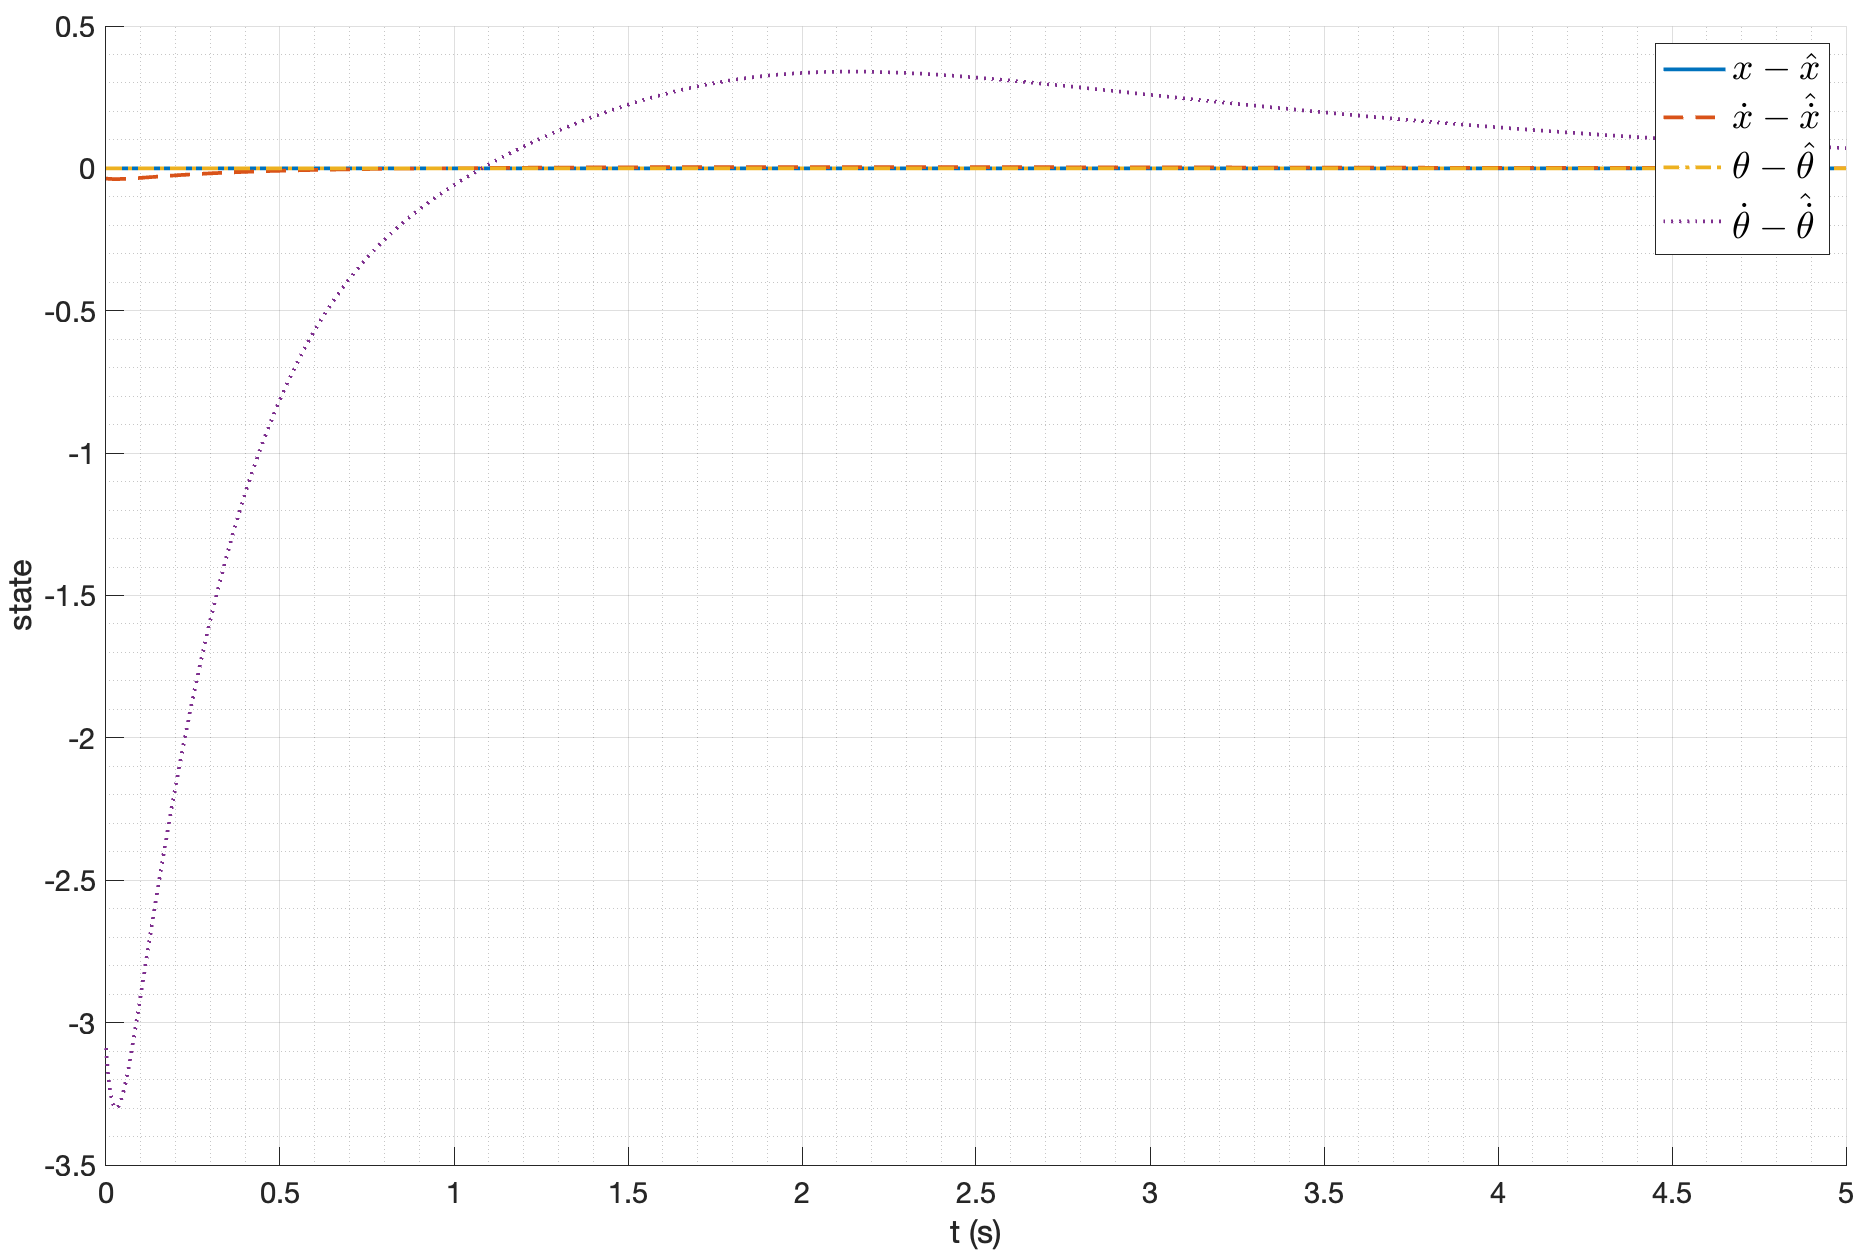
\includegraphics[width=\textwidth]{media/plots/reduced_observer/reduced_observer_err_2.png}
    \caption{Ошибка оценки состояния системы наблюдателем пониженного порядка}
    \label{fig:reduced_observer_err_2}
\end{figure}
\FloatBarrier
Так же видно, что два измеримых состояния системы совпадают с реальными значениями, а два
неизмеримых состояния системы тоже сходятся к реальным значениям, но с большим временем переходного процесса,
которое составляет около 2.5 секунд.

% Проведем сравнение наблюдателей полного и пониженного порядка со спектрами $\{-4, -4, -4, -4\}$ и $\{-4, -4\}$ соответственно.
% TODO: compare observers

\subsection{Регулятор по выходу}
Рассмотрим реальный случай, когда для измерения и использования доступны только 
два из четырех состояний системы, а именно координата тележки и угол отклонения маятника.
Эти состояния могут быть измерены с помощью датчиков, установленных на системе. Для того, чтобы
стабилизировать систему будем использовать регулятор, основанный на оценке состояния системы 
наблюдателем пониженного порядка. 

Порядок синтеза модального регулятора и наблюдателя пониженного порядка приведен выше. 
Схема моделирования приведена на рисунке \ref{fig:modal_controller_obderver}.
Выход подсистемы, соответствующий вектору состояния не используется, что 
имитирует реальный случай, когда для управления доступны только два состояния системы. 

\begin{figure}[ht!]
    \centering
    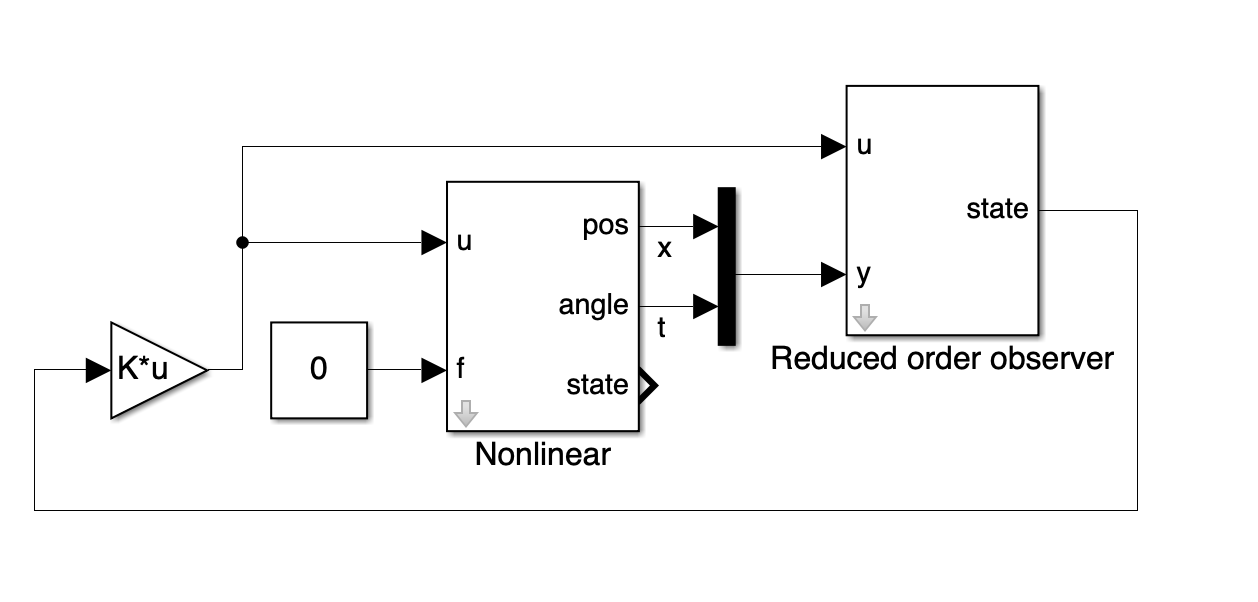
\includegraphics[width=0.7\textwidth]{media/model_controller_observer.png}
    \caption{Схема моделирования регулятора по выходу}
    \label{fig:modal_controller_obderver}
\end{figure} 

Подберем спектры регулятора и наблюдателя пониженного порядка таким образом, чтобы 
достичь наилучшего качества переходного процесса. Наилучшего результата удалось достичь при
спектрах $\{-9, -9, -9, -9\}$ и $\{-5, -5\}$ для регулятора и наблюдателя соответственно. 
Выход системы, замкнутой регулятором по выходу, приведен на рисунке \ref{fig:modal_controller_obderver_out}.
\begin{figure}[ht!]
    \centering
    \includegraphics[width=\textwidth]{media/plots/observer_controller/observer_controller_out.png}
    \caption{Результаты моделирования регулятора по выходу}
    \label{fig:modal_controller_obderver_out}
\end{figure}

Система стабилизируется, при этом время переходного процесса составляет около 1.8 секунд. 
График управляющего воздействия приведен на рисунке \ref{fig:modal_controller_obderver_u}.
\begin{figure}[ht!]
    \centering
    \includegraphics[width=\textwidth]{media/plots/observer_controller/observer_controller_u.png}
    \caption{Управляющее воздействие регулятора по выходу}
    \label{fig:modal_controller_obderver_u}
\end{figure}
Максимальное по модулю управляющее воздействие составляет около 15000 Н. Величина, довольно большая, 
но может быть объяснена тем, что масса тележки составляет 255кг. 

\FloatBarrier
\subsection{Выводы} 
В данной главе были рассмотрены модальные регуляторы и наблюдатели. Были рассмотрены влияния собственных 
чисел замкнутой системы на динамику системы, а также влияние собственных чисел на работу наблюдателя. 
Исследовано влияние начальных условий на работу системы. Ожидаемым результатом оказалось то, что 
при увеличении модуля собственных чисел замкнутой системы, время переходного процесса уменьшается, 
при этом увеличивается перерегулирование и максимальное по модулю управляющее воздействие. 
Влияние начальных условий на работу системы оказалось тоже весьма ожидаемым. При увеличении 
начального отклонения маятника увеличивается расхождение между линеаризованной моделью и реальной системой, 
что приводит к ошибкам в управлении. Начиная с некоторого значения начального отклонения, 
на практике оказавшегося равным 1.2 радиан, система не может быть стабилизирована. 